%%%%%%%%%%%%%%%%%%%%%%%%%%%%%%%%%%%%%%%%%%%%%%%%%%%%%%%%%%%%%%%%%%%
%                                                                 %
%                            ROOT FILE                            %
%                                                                 %
%%%%%%%%%%%%%%%%%%%%%%%%%%%%%%%%%%%%%%%%%%%%%%%%%%%%%%%%%%%%%%%%%%%
%
%  Run LaTeX or pdfLaTeX on this file to produce your thesis.
%  To produce the abstract title page followed by the abstract,
%  see the file abstitle-phd.tex or abstitle-mas.tex.
%
%%%%%%%%%%%%%%%%%%%%%%%%%%%%%%%%%%%%%%%%%%%%%%%%%%%%%%%%%%%%%%%%%%%

\documentclass[chap]{thesis}

%%%%%%%%%%%%%%%%%%%%%%%%%%%%%%%%%%%%%%%%%%%%%%%%%%%%%%%%%%%%%%%%%%%

\usepackage{graphicx}
\graphicspath{ {resources/} }

%\usepackage{amsmath}
%\usepackage{amsthm}
%\usepackage{amssymb}
\usepackage[usenames,dvipsnames,svgnames,table]{xcolor}
\usepackage{pdfpages}
\usepackage{tikz}
\usepackage{amsmath}
\usepackage{amssymb}
\usepackage[numbers]{natbib}
\usepackage[labelfont=bf]{caption}
\usepackage[labelformat=simple]{subfig}
\usepackage{mathtools}


\DeclarePairedDelimiter\ceil{\lceil}{\rceil}
\DeclarePairedDelimiter\floor{\lfloor}{\rfloor}

\newcommand*{\head}[1]{%
	\textbf{#1}
}
\newcommand{\cnote}[1]{%
	{\color{red}[#1]}
}
\renewcommand{\textfraction}{0.01}
\renewcommand{\floatpagefraction}{0.99}
\renewcommand{\topfraction}{0.99}
\renewcommand{\bottomfraction}{0.99}
\renewcommand{\dblfloatpagefraction}{0.99}
\renewcommand{\dbltopfraction}{0.99}
\renewcommand{\th}{$^{th}$}
\newcommand{\conv}{\mathop{\scalebox{1.2}{\raisebox{-0.2ex}{$\ast_{x,y}$}}}}

%%%%%%%%%%%%%%%%%%%%%%%%%%%%%%%%%%%%%%%%%%%%%%%%%%%%%%%%%%%%%%%%%%%

\begin{document}

    %%%%%%%%%%%%%%%%%%%%%%%%%%%%%%%%%%%%%%%%%%%%%%%%%%%%%%%%%%%%%%%%%%%
%                                                                 %
%                            TITLE PAGE                           %
%               Master's Thesis or Master's Project               %
%                                                                 %
%%%%%%%%%%%%%%%%%%%%%%%%%%%%%%%%%%%%%%%%%%%%%%%%%%%%%%%%%%%%%%%%%%%

% Supply information for use on title page:
\thesistitle{\bf Online Architectural Sketching Interface for Simulations}
\author{Max\ Espinoza}
\degree{Master of Science}
\department{Computer Science}

\signaturelines{3}
\projadviser{Dr. Barbara Cutler}
\memberone{Dr. Charles Stewart}
\membertwo{Dr. Randolph Franklin}

\submitdate{March 2016\\(For Graduation May 2016)}
\copyrightyear{2015}   % if omitted, current year is used.

% Print titlepage and other prefatory material:
\titlepage
\copyrightpage         %optional
\tableofcontents
\listoftables          %required if there are tables
\listoffigures         %required if there are figures


    \newpage

    %%%%%%%%%%%%%%%%%%%%%%%%%%%%%%%%%%%%%%%%%%%%%%%%%%%%%%%%%%%%%%%%%%%
%                                                                 %
%                         ACKNOWLEDGEMENTS                         %
%                                                                 %
%%%%%%%%%%%%%%%%%%%%%%%%%%%%%%%%%%%%%%%%%%%%%%%%%%%%%%%%%%%%%%%%%%%

\specialhead{ACKNOWLEDGMENTS}

\textit{The Great Zebra \& Giraffe Count} (GZGC) was powered and administered by the IBEIS team with notable help from Dr.\ Paula Kahumbu and staff at Wildlife Direct in Nairobi, Kenya.  The IBEIS team would like to thank the people and government of Kenya for supporting this research (Permit \# NACOSTI/P/14/1003/1628), with special recognition to Senior Warden of the Nairobi National Park, Nely Palmeris, and Macharia ``Michael'' Kimura of the Kenyan Wildlife Service (KWS).  Other contributions to this thesis were provided by Clara Machogu, Marco Maggioni, Jon Crall, Hendrik Weideman, Michael Brown, and Zachary Jablons.  I would like to thank Dr.\ Tanya Berger-Wolf, Dr.\ Daniel Rubenstein, and my master committee members, Dr.\ Barbara Cutler and Dr.\ B{\"u}lent Yener, for their valuable feedback.  I would also like to give a special thank you to my Ph.D.\ advisor, Dr.\ Charles Stewart, who has patiently guided me to this milestone of my academic career.

All of the software detailed in this thesis can be downloaded from open-source code repositories.  The IBEIS software can be downloaded on GitHub \footnote{github.com/erotemic/ibeis [Accessed: Nov. 1, 2015]} and the client-server code used during the GZGC data collection event can also be downloaded on Github \footnote{github.com/bluemellophone/[gzc-client, gzc-server] [Accessed: Nov. 1, 2015]}.  The open-source software and research detailed in this thesis was supported by Rensselaer Polytechnic Institute (RPI) and with financial support from NSF EAGER Grant (Award \#1453503) \textit{Collaborative Research: EAGER: Prototype of an Image-Based Ecological Information System (IBEIS)}.

Lastly, but most importantly, I would like to thank my wife, Lindsay, for providing patient, never-failing support.  Her dedication to my academic career and intellectual progress has been the best example of sacrificial love I have ever had the privilege to personally experience.

\begin{figure}[!htb]%
    \centering
    \subfloat {{ $\vcenter{\hbox{ \includegraphics[height=0.15\textwidth]{resources/logo_ibeis.png} }}$ }}%
    \qquad
    \subfloat {{ $\vcenter{\hbox{ \includegraphics[height=0.12\textwidth]{resources/logo_wd_alpha.png} }}$ }}%
\end{figure}


    \newpage

    %%%%%%%%%%%%%%%%%%%%%%%%%%%%%%%%%%%%%%%%%%%%%%%%%%%%%%%%%%%%%%%%%%%
%                                                                 %
%                            ABSTRACT                             %
%                                                                 %
%%%%%%%%%%%%%%%%%%%%%%%%%%%%%%%%%%%%%%%%%%%%%%%%%%%%%%%%%%%%%%%%%%%
\specialhead{ABSTRACT}
Daylighting plays a significant role in architecture; its creative and efficient use offers aesthetics visuals, increased productivity, and energy savings. However, poor implementation of daylighting systems can have adverse impacts such as visual discomfort, solar heat gain, and an absence of energy savings. 

As a result, architects turn to daylighting analysis as means to predict daylighting's effects on architectural spaces prior to construction. However, there are several challenges in daylighting analysis, that make prediction non-trivial and time intensive. Specifically, there are numerous factors to consider when visualizing the natural lighting of an interior space. Daylight can vary depending on the season, the time of day, the cardinal direction of fenestrations,  the geographic location and geometry the space,  the reflectance of interior materials, and more.  

The traditional approaches to solving this problem require either the construction of physical scale model or development of virtual 3D models. Both methods are time intensive and can cause delays in the fast-paced schematic design phase of architecture.  

I present a novel interface that is easily accessible to non-experts providing them with the ability to generate 3D models for daylighting simulation from 2D architectural sketches. This online interface allows users to both quickly create 3D models and analysis daylighting simulation results. I propose that this interface will aid both experts and non-experts during the schematic design phase where ease of expressing 3D geometries and speed of analyzing simulation results is most significant. 

My contributions includes the development of this online interface, the conduction of a large-scale user study, and the analysis of that study.

    %%%%%%%%%%%%%%%%%%%%%%%%%%%%%%%%%%%%%%%%%%%%%%%%%%%%%%%%%%%%%%%%%%%
%                                                                 %
%                            CHAPTER ONE                          %
%                                                                 %
%%%%%%%%%%%%%%%%%%%%%%%%%%%%%%%%%%%%%%%%%%%%%%%%%%%%%%%%%%%%%%%%%%%

\chapter{INTRODUCTION} \label{sec:introduction}

Daylighting is the use of natural light and building geometry for aesthetically pleasing visuals and the creation of productive environments.
However, daylighting is much more than just pleasing visuals and productive environments.
Daylighting is also an environmental sustainability design practice for the creation of greener buildings and reduction power consumption.
Similarly, daylighting can also be seen an  economic means to reduce a building energy demands or increase worker productivity to generate capital.
Despite the variety of definitions, daylighting will always refer to the use of daylight to met an architectural purpose.

% Overview 
Firstly, to understand what drives daylighting research a brief overview of daylight's advantages is necessary.
In short, daylight is mainly valued as a source of illumination however recent studies show that daylight also offers economic and health benefits.
%
Secondly, I explain why architects struggle with the design of daylighting systems.
By and large, daylighting is challenging by virtue sunlight's dynamic nature.
Moreover, daylight used incorrectly can cause occupants both visual and thermal discomfort.
%
Lastly, I review architectural practices used in the design of daylighting system for the purpose of better following the advances .
Briefly, architects exercise sketching techniques, follow rules-of-thumb, and consult daylighting visualizations to help guide the design of effective daylighting systems. 
%
All things considered, the motives that drive architects and building owners to employ daylighting systems also drive researchers to developer better tools for the design and analysis of daylight in architectural spaces.\\

% This section is basically done
\section{Benefits And Motivations Of Daylighting Systems}
    
  % Our small intro into the next few pages of motives
  There are many benefits to using daylight over traditional electrical lighting.
  Recent studies show exposure to sunlight, offered readily through daylighting systems, has a variety of health benefits; benefits such as the stimulation of vitamin D production and maintenance of healthy circadian rhythms.
  In addition to health-related benefits there are economic motives that drive architects and building owners to to implementing daylighting systems.
  Some economic motives include increases in worker productivity and overall reduced building energy demands.
  In short, daylighting system offer both economic incentives for building owners and health benefits for occupants.

  % TODO: Requires proof reading
  \subsection{Vitamin D}
    Vitamin D is an essential fat-soluble secosteroid required for healthy human functions. It aids in the absorption of calcium and other minerals. Vitamin D plays a significant role in the mineralization of bone\cite{Ross}.   
    Prolonged vitamin D deficiency can result in many serious diseases.
    Adults suffering from vitamin D deficiency can develop osteomalacia -- the softening of bones. Children deprived of vitamin D can develop harmful diseases such as rickets. Children diagnosed with Rickets suffer from poor bone mineralization and are prone to bone fractures and deformity\cite{Pettifor}. \\

    There are many may to meet daily vitamin D requirements. For example, skin tissue is capable of creating vitamin D on its own, certain foods contain high concentrations of the vitamin, and dietary supplements fortified with vitamin D are readily available\cite{Ross}.
    Human skin has a built-in mechanism that helps synthesis vitamin D through the exposure of Ultra Violet(UV) light. Light rich in UV hitting the surface of the skin will begin the processes of vitamin D synthesis. Synthesis through the exposure to sunlight meets most daily vitamin D requirements. Foods we consume are usually rich in vitamin and minerals. However, vitamin D occurs in significant concentrations in very few natural food items, such as fatty fish, particular species of mushrooms, and beef liver.  Because of vitamin D's scarcity in naturally occurring food items and the harmful effects of deficiency vitamin D  in children, companies fortify common breakfast food with vitamin D -- such as orange juice, milk, and cereals. Lastly, Vitamin D can also be taken in pill form as a deity supplement. \\

    Working typical office hours in windowless environments decrease exposure to daylight and increases the risk of vitamin D deficiency. Living an indoors lifestyle coupled with the widespread usage of sunscreen products created a vitamin D deficiency pandemic.  Our skin does not synthesize vitamin D efficiently. Wearing sunscreen with an SPF of 15 absorbs 99\% of UVB radiation and consequently, reduce the ability to synthesize vitamin D by as much as 99\%\cite{Holick}. \\

    Architectural daylighting can help alleviate this risk by creating buildings with apertures and geometry that promote deep penetration of natural lighting into a building's interior. Daylight is rich in UV radiation required for vitamin D synthesis.  Daylighting systems could, in theory, help occupants keep occupants healthy by passively enabling occupants to meet their daily vitamin D requirements. \\

  % TODO: Requires proof reading
  \subsection{Circadian Photobiology}
    Daylighting has influence over our circadian photobiology. Circadian photobiology is the human experience hormonal and behavioral changes throughout a roughly 24-hour cycle. The hypothalamic suprachiasmatic nucleus (SCN)  in the brain, which relies on input from non-rod/non-cone photoreceptor systems located in our retina, regulates these non-image forming light responses. These non-rod/non-cone photoreceptors are excited by exposure to alternating periods of light and dark. They specifically respond to lighting conditions found in daylight\cite{Rea,Thapan}.\\

    Electrical lighting varies from daylight a couple of biologically important ways\cite{Rea}. Daylight offers a higher levels of illumination, a wider spectrum of electromagnetic radiation, and a temporal variation in lighting. Firstly, sunlight in conjunction with skylight, measures anywhere between 10 to 100 thousand lux\cite{Robbins}. However, the government agency of Occupational Safety and Health Administration (OSHA) set 322 lux as the minimum of lighting requirement for typical office work\cite{OSHA}. Lighting conditions that do not excite photoreceptors responsible for maintaining our circadian rhythm are essentially biological darkness\cite{Leslie}. Secondly, the spectrum of light emitted by artificial lighting lacks short wavelength electromagnetic radiation found in sunlight.Varying wavelengths of electromagnetic radiation affects melatonin levels in humans as much as varying intensity of light. Melatonin suppression is necessary because it plays a role in sleep-wake cycles, body temperature regulation, alertness, and blood pressure\cite{Gooley}. Studies show melatonin suppression varies most through exposure to short wave electromagnetic radiation \cite{Brainard}. Consequently, daylighting systems offer the advantage of exposure to short wavelength electromagnetic radiation needed for melatonin suppression. Lastly, exposure to light during periods of the day asynchronous to our circadian rhythm can result in shifts in our sleep-wake cycles. These shifts, known as phase shifts, triggers melatonin suppression at particular times. For instance,  morning light exposure triggers melatonin suppression resulting in the feeling of alertness\cite{Rea}. However, exposure to light at asynchronous times of day results in a phase shift. An unexpected phase shift can have symptoms similar to jet lag and significantly hinder productivity\cite{Rea}. Daylight availability during those crucial morning hours could potentially have significant impacts on employee productivity. \\

  % TODO: Requires proof reading
  \subsection{Increased Productivity}
    Studies show daylighting systems increase both the productivity and comfort of occupants\cite{Menzies}.  Daylighting increases workplace productivity and satisfaction through a variety of means. To begin, the human eye as image processing system has evolved over millions of years to work optimally under full spectrum illumination provided by sunlight and skylight. It is not surprising that the human visual system works better using daylight as a source of light. A visual task, such as reading, generally require less illumination when using daylight as opposed to electrical lighting\cite{Robbins}. Additionally, daylight provides superior color rendering. Our visual system is tuned to differentiate colors under full spectrum illumination. Differentiating colors under low illumination or fluorescent lighting is not as reliable as compared to daylight\cite{Robbins}. There are current electrical lighting systems that provide full spectrum light, however, these systems are very costly when compared to daylight. Moreover, occupants enjoy being near windows since it gives them information about their outdoor environment -- including the time of day, weather conditions outdoors, and activities happening outside. Having a workstation near a window could evoke a feeling of importance in occupants. This feeling of importance increases worker satisfaction and could possible increase productivity\cite{Leslie}. Overall, the satisfaction of occupants is important to architects and managers, because adverse environmental factors hinder productivity in a workspace.  \\

    These gains provide a financial benefits to companies investing in daylighting systems. However, focus groups and interviews with professionals conducted show that architects prioritize the comfort and productivity of a building’s inhabitants over a building’s sustainability\cite{Menzies}. Meaning building designers see daylighting as means to make occupants comfortable through use of natural lighting, rather than as a eco-friendly lighting system. \\

  % TODO: Requires proof reading
  \subsection{Reduced Energy Demands}
    There are direct economic gains from daylighting systems. Energy saving from reducing electrical illumination use save building owners money.
    It is important to note that daylighting systems do not directly save capital, rather daylighting systems give building owners the opportunity to conserve energy by using sunlight as an alternative or supplement to electric illumination. Electricity companies charge peak hour rates during the afternoon when demand for electricity is highest. During these hours alternatives sources of light, such as daylighting, become cost effective.
    It is hard to estimate how much energy savings with daylighting systems. Simulations are an important tool architects use to determine energy cost saving during the design development processes.  Lighting usually accounts for about 25-40\% of a total building energy demands.
    According to one study daylight can save up to 52\% of energy on a wall adjacent to a window\cite{Leslie}.\\

    Using daylight as an alternative or supplement to electrical lighting requires some form of daylight management. Daylighting management requires dimming systems that dim electrical lighting during the peak hours when daylight is most available.  Some simulation results show that when there no lighting management in place,  power consumption from lighting can exceed 50\% of a building's total power demand.
    However, those simulations also show daylighting can save a building up to 18\% to 55\% of a building heating and lighting demand\cite{Bodart}.
    Without a dimming system, the window of time in which daylighting is cost effective is significantly smaller. Other simulation results showed energy savings of 60\% with daylighting and dimming control strategies\cite{Ihm}. \\

    Also, dimming lights result in reduced thermal output from lighting fixtures. Which in turn reduces the total cooling load required in space. The reduced cooling load also contributes to energy saving in daylighting systems\cite{Leslie}. In addition to reducing the cooling load, daylighting can also be used for heat gains during the winter. Daylighting systems exploit the shallow sun angle in the winter months and allow winter sunlight into a building. Heating a large space is expensive, and sunlight can aid in heating\cite{Bodart}. \\

% This requires some work
\section{Challenges Of Designing Daylighting Systems}
  
  % Unsure of apostrophe in "outnumbers design' affect"
  Daylight has many benefits over traditional electrical lighting, however,reaping those benefits is not effortless. There are many factors architects have to consider when designing a daylighting system. Choices made during the early stages of design can have extensive impact on the effectiveness of a daylighting system. Likewise, design choices can also result in visual discomforts for occupants and economic loss for building owners. By and large, architects planning daylighting systems are required to analyze numerous designs' affect on daylight. Furthermore, architects have to be cautious of sunlight's dangers to both occupants and building owners.

  \subsection{Factors That Affect Daylighting}

    % [Introduction]
    Illumination of an architectural space via daylight is dependent on numerous factors including building-wide design choices, room-specific choices, and temporal variations.
    These factors make it difficult to access the quality of a design in terms of daylighting.\\

    \paragraph{Building-wide Design Choices} 
    The cardinal orientation of a building is a choice that directly affect how daylight will illuminate architectural spaces. In the northern hemisphere, windows facing the south cardinal direction experience direct daylight throughout the day. On the other hand, north facing windows do not experience this effect. Rather north facing windows experience indirect diffuse illumination from the sky. The opposite is true in the southern hemisphere. In the south, north facing windows experience direct daylight and south facing windows experience diffuse indirect light. Likewise, windows facing east experience morning sunlight and windows facing west experience evening sunlight. Variations in eastward and westward lighting are a result the sun's eastwards to westwards path across the sky\cite{Robbins}. See Figure~\ref{fig:north_south} for an illustration.

    \begin{figure}[h]
      \centering
      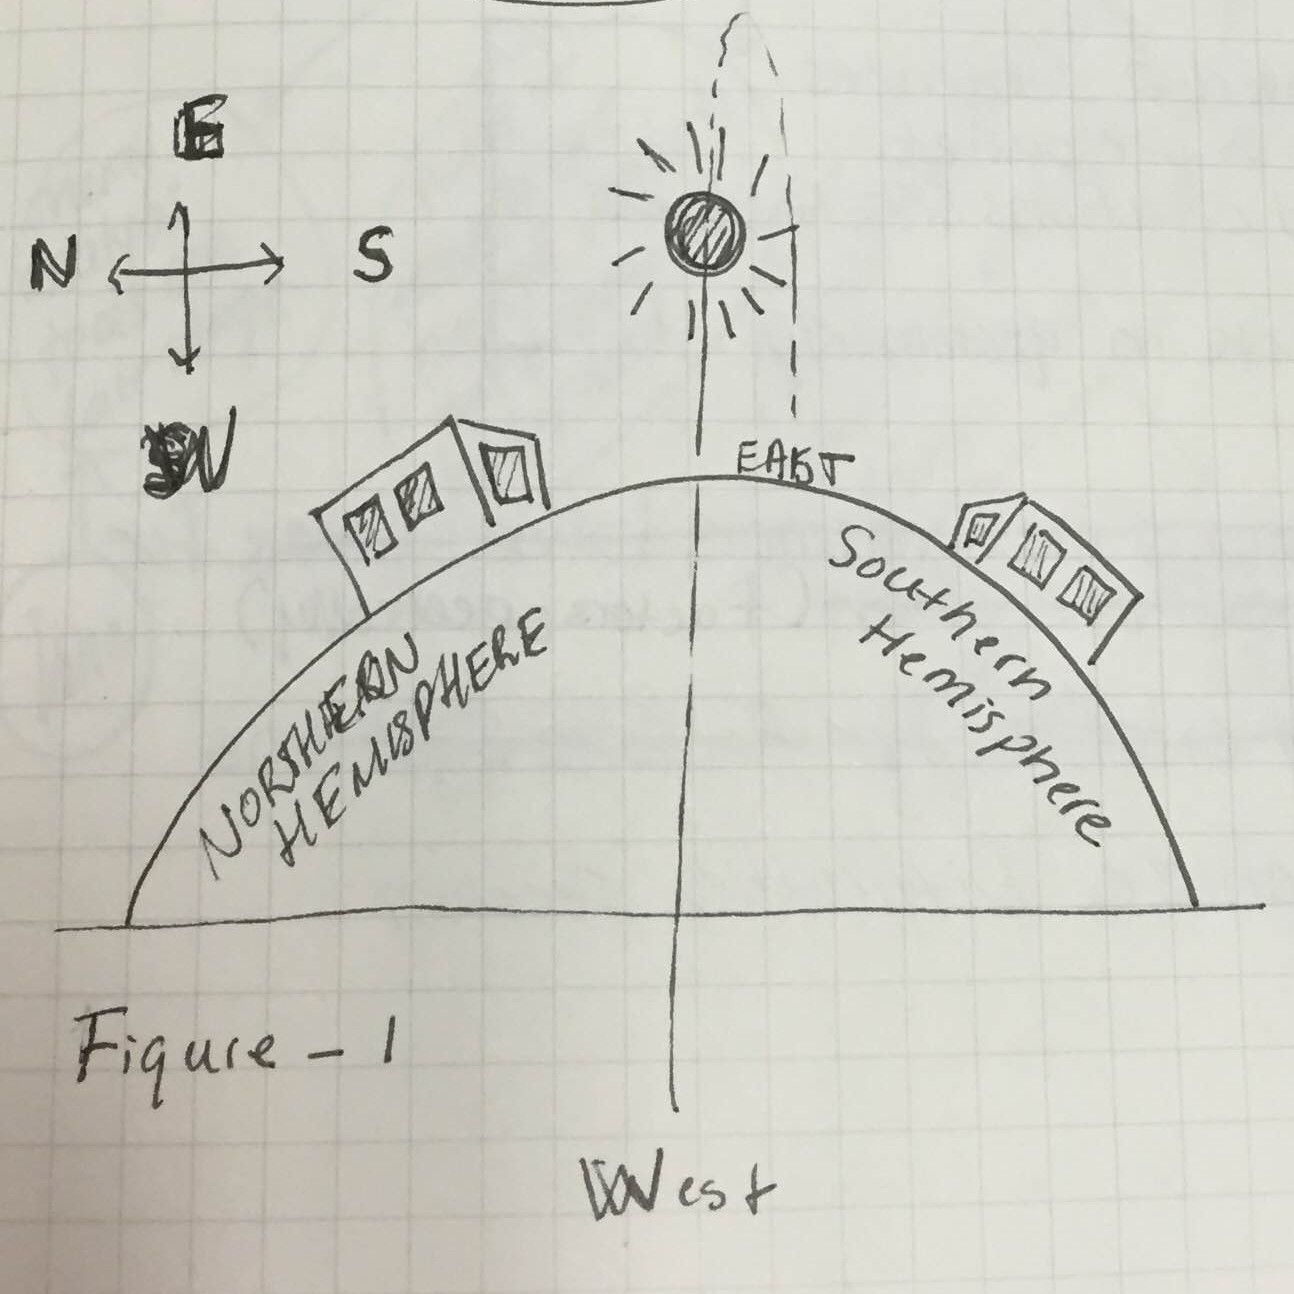
\includegraphics[width=0.25\textwidth]{north_south_fig}
      \caption{This illustration shows why windows facing southward in the northern hemisphere experience direct daylight and windows facing northward do not. It also shows the converse, north facing windows in the southern hemisphere experience direct lighting, however those facing southward do not.} 
      \label{fig:north_south}
    \end{figure}

    Aside from building orientation, building elevation can affect daylighting as well. Varying building elevation can change how daylight illuminates an architectural space. For example, a building located well above sea level will experience a slight difference in daylighting compared to a building below sea level. Daylight usually enters a space either perpendicular to a flat window pane or at a downwards angle starting from the Sun and ending at the floor and walls. However, a skyscraper could potentially have daylight enter a space at an upwards angle towards the ceiling due to its increased elevation.\\


    \begin{figure}[h]
      \centering
      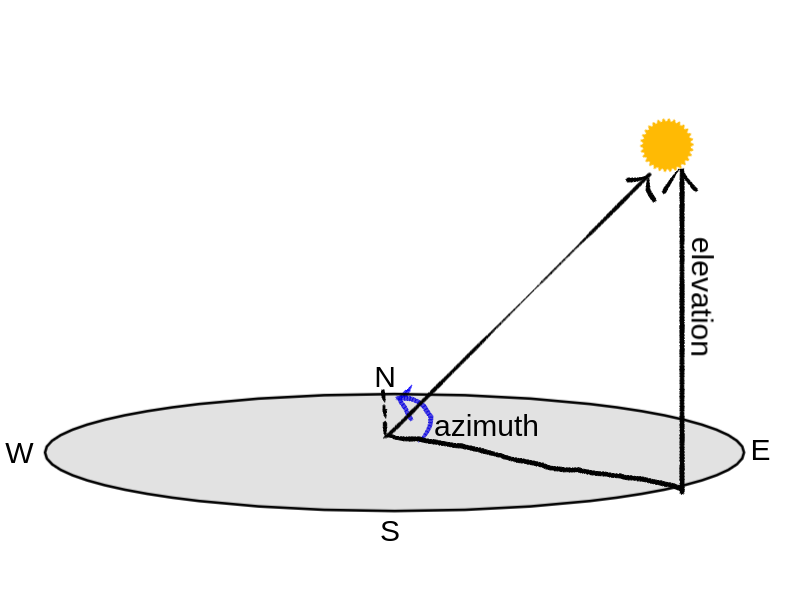
\includegraphics[width=0.5\textwidth]{sun_position}
      \caption{Illustration to show elevations and azimuth used to find the sun's position in the sky} 
      \label{fig:sun_position}
    \end{figure}

    \begin{equation} \label{eq:elevation}
    E = sin^{-1}(sin(\delta) sin(\phi) + cos(\delta) cos(\phi) cos(HRA))
    \end{equation}
    \begin{equation} \label{eq:azimuth}
    A = cos^{-1}( \frac{sin(\delta) cos(\phi) - cos(\delta) sin(\phi) cos(HRA)}{cos(E)})
    \end{equation}

    Just as important as building orientation and elevation, where a building is geographically built has direct impact on daylighting.
    Specifically, the path the sun travels across the sky varies with geographic location and time. 
    Equation-\ref{eq:elevation} and equation-\ref{eq:azimuth} are commonly used in daylighting to calculate the sun's position in the sky. 
    The elevation angle, given by Equation-\ref{eq:elevation}, is the angle between the horizon and solar zenith, as illustrated in figure~\ref{fig:sun_position}. 
    $\delta$ in  equation-\ref{eq:elevation} and equation-\ref{eq:azimuth} refers to the solar declination angle. 
    Lastly, $\phi$ is the latitude of interest in both equations and $HRA$ is the hour angle in local solar time.
    The azimuth angle, as shown in figure-\ref{fig:sun_position}, is the angle between the cardinal north direction and the direction the sun projected down towards the horizon. The azimuth can be found once the elevation angle has been found, as show in equation-\ref{eq:azimuth}.
    As shown in both equations, the suns position in the sky is relative to longitude, latitude, and temporal variables.\\

    % [Building design decisions]
    \paragraph{Room-specific Design Choices} 

    Room-specific design choices also have an impact on the daylight.
    The geometry of an interior space directly affects the distribution of daylight in a room.
    Geometries can be designed to diffuse direct lighting for uniform illumination and occupant comfort.
    Similarly, shading devices and material properties of interior objects can affect daylighting.
    Shading devices, such as blinds can not only help diffuse direct lighting but also help redirect lighting up towards the ceiling, where it can be diffusely reflected back down towards occupants.
    Also, a careful selection of both the color and the material of interior items such furniture, walls, and ceiling can affect daylight's distribution in an interior space. 

    \begin{figure}[h]
      \centering
      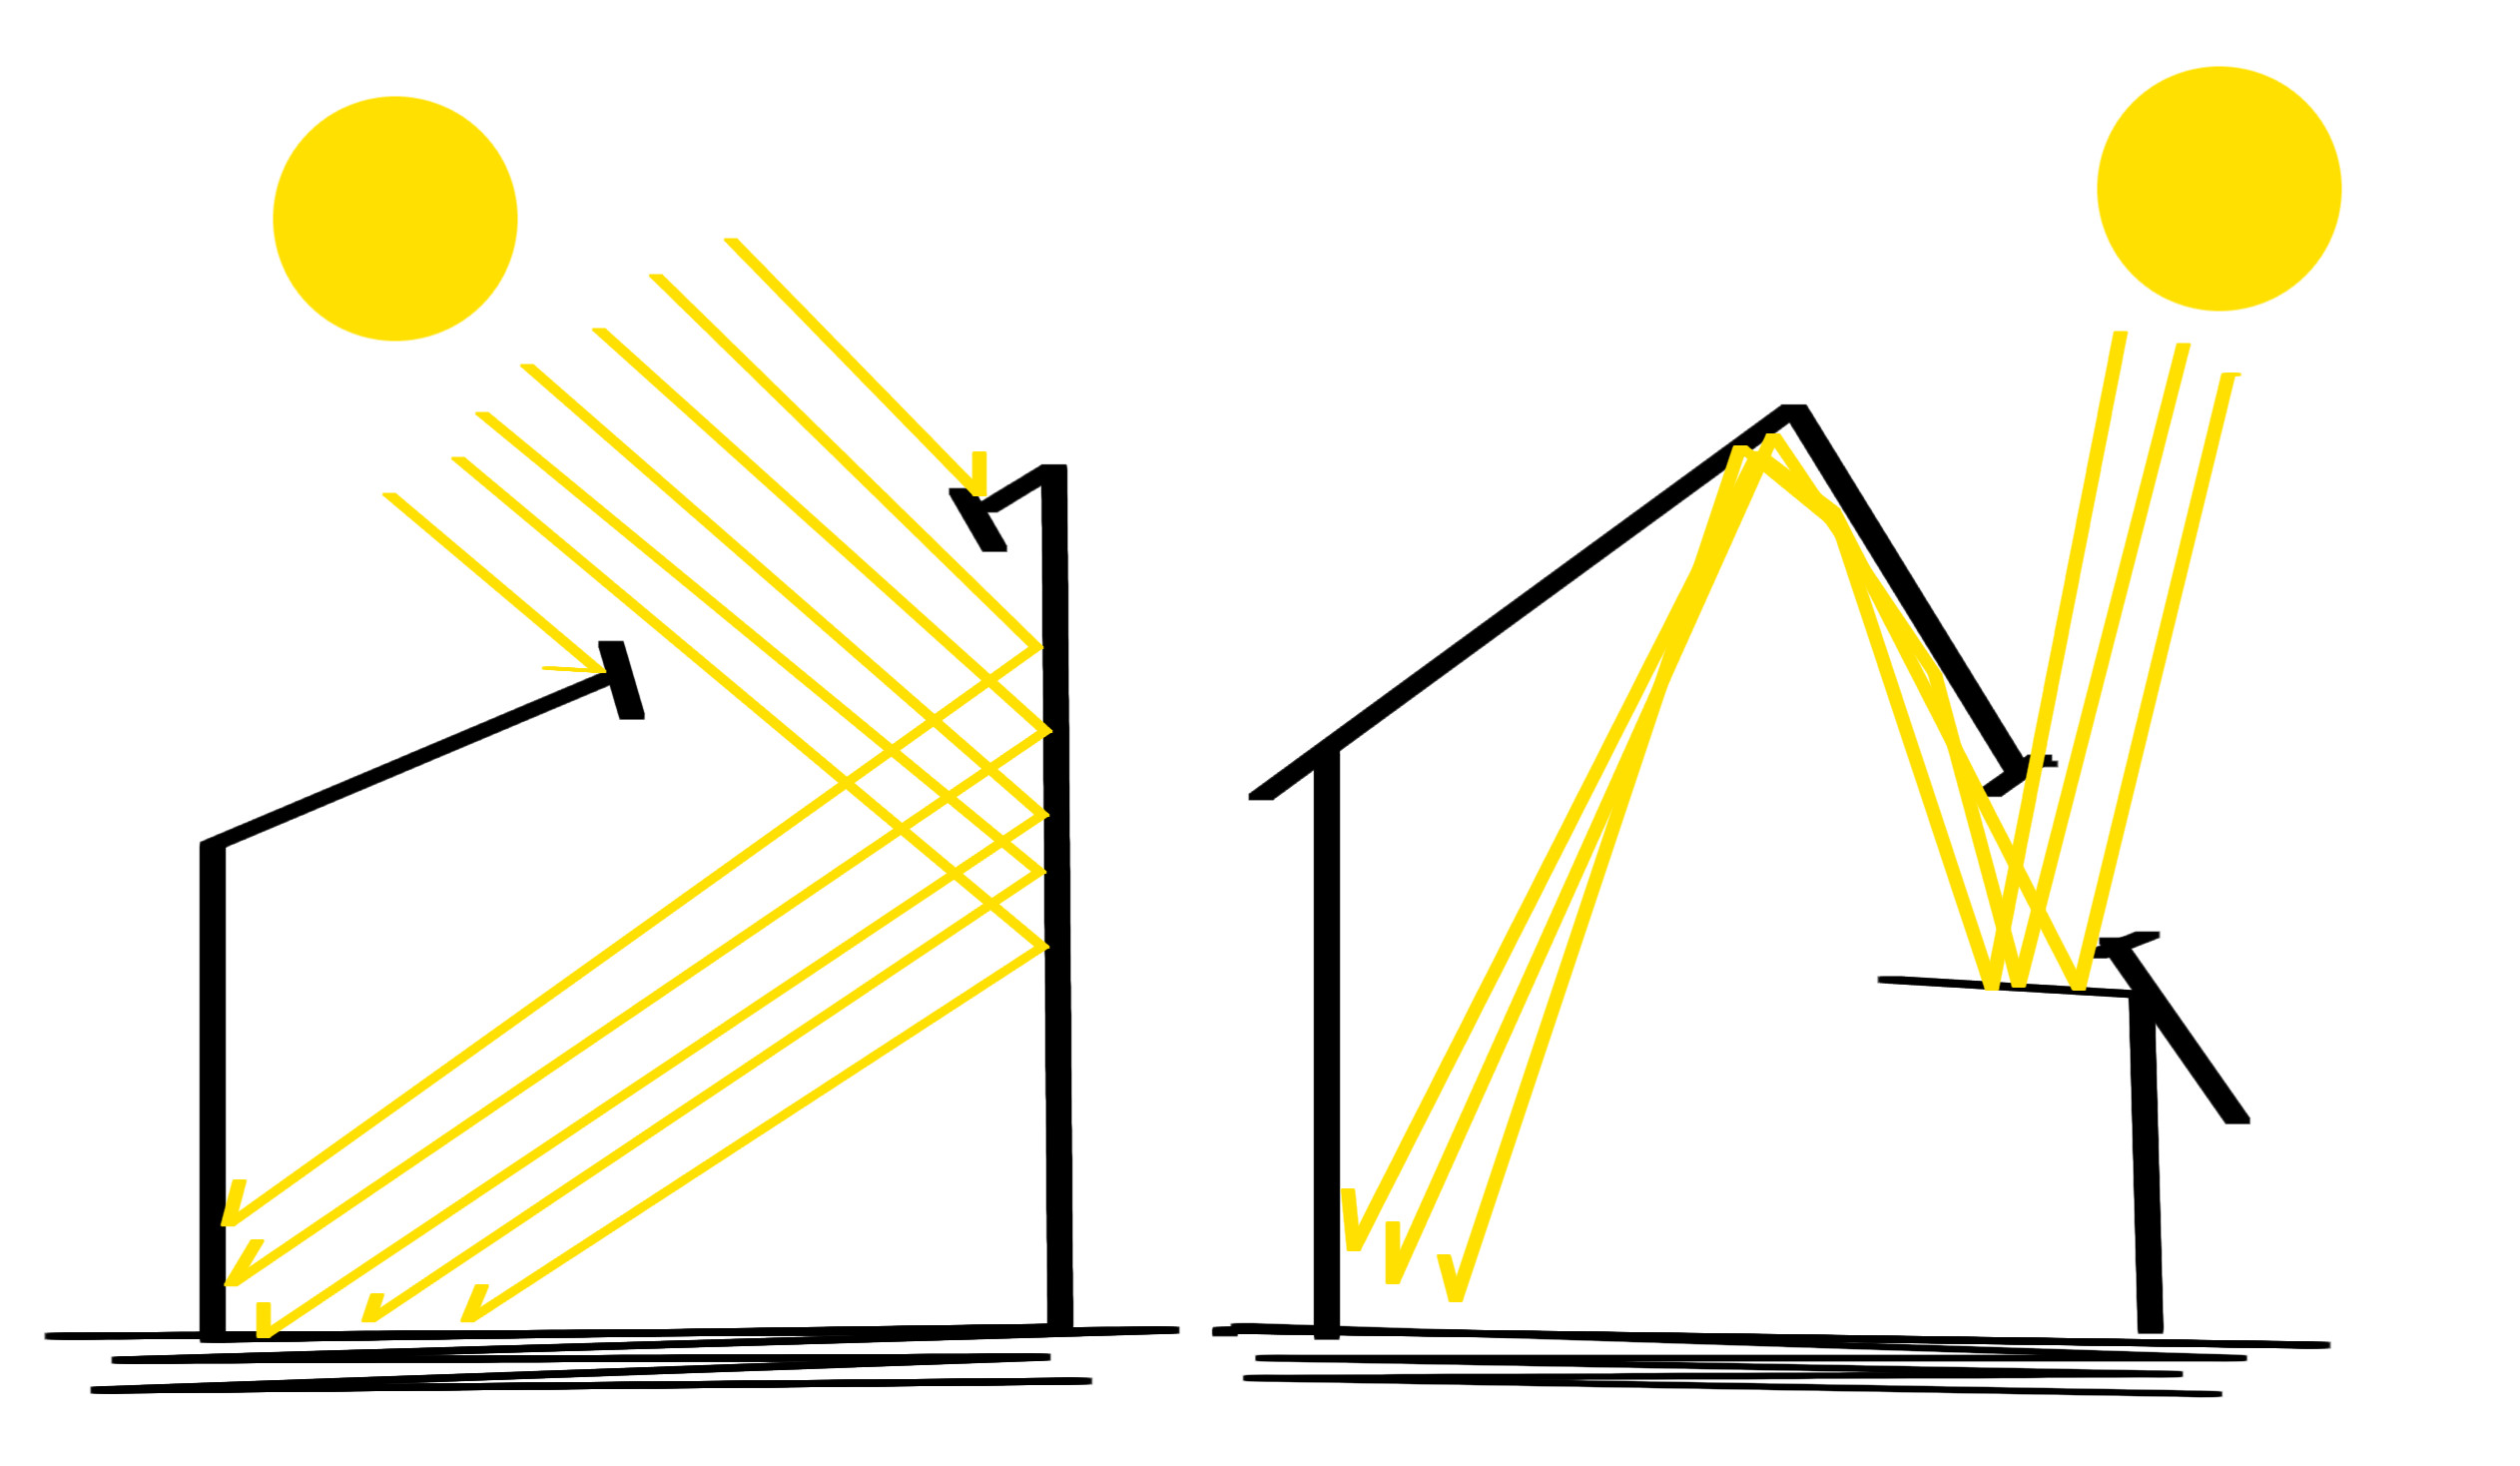
\includegraphics[width=0.5\textwidth]{geometry_sketch}
      \caption{Left: a common skylight placement on the roof of a building. The angled roof is designed to let daylight diffuse as it reflects on towards the floor. Right: A light shelf that helps redirect daylight up towards the ceiling, where it can be diffused and reflected back down on towards the floor.}
      \label{fig:geometry_sketch}
    \end{figure}

    In addition to material and shading devices, window placement and size directly influence daylighting.
    Larger windows and skylights allow more light to enter a space, however, poses the risk of over-illumination and glare for occupants inside.
    Likewise, the glazing material used to treat windows can also be used to control the amount and distribution of daylight entering a space.
    The glass used in commercial buildings are glazed to block a significant portion of light from entering a space.
    Glazing are used because direct sunlight would cause over-illumination, thermal discomfort, and harm to the occupants situated near windows.
    Special glazing can also be used to help diffuse lighting up towards the ceiling and away from occupants.
    The choices that architects make in room-specific design significantly affect the daylighting.\\

    % [Temporally]
    \paragraph{Temporal Variation} 

    It is obvious that daylight varies from sun raise to sun set.
    Less obviously, daylight also varies throughout the year.
    The Sun's position in the sky is shallower during winter season than in the summer season. 
    Due to this, during the winter months daylight enters a room at a shallower angle allowing light to travel deeper than in the summer months.

    \begin{figure}[h]
    \centering
    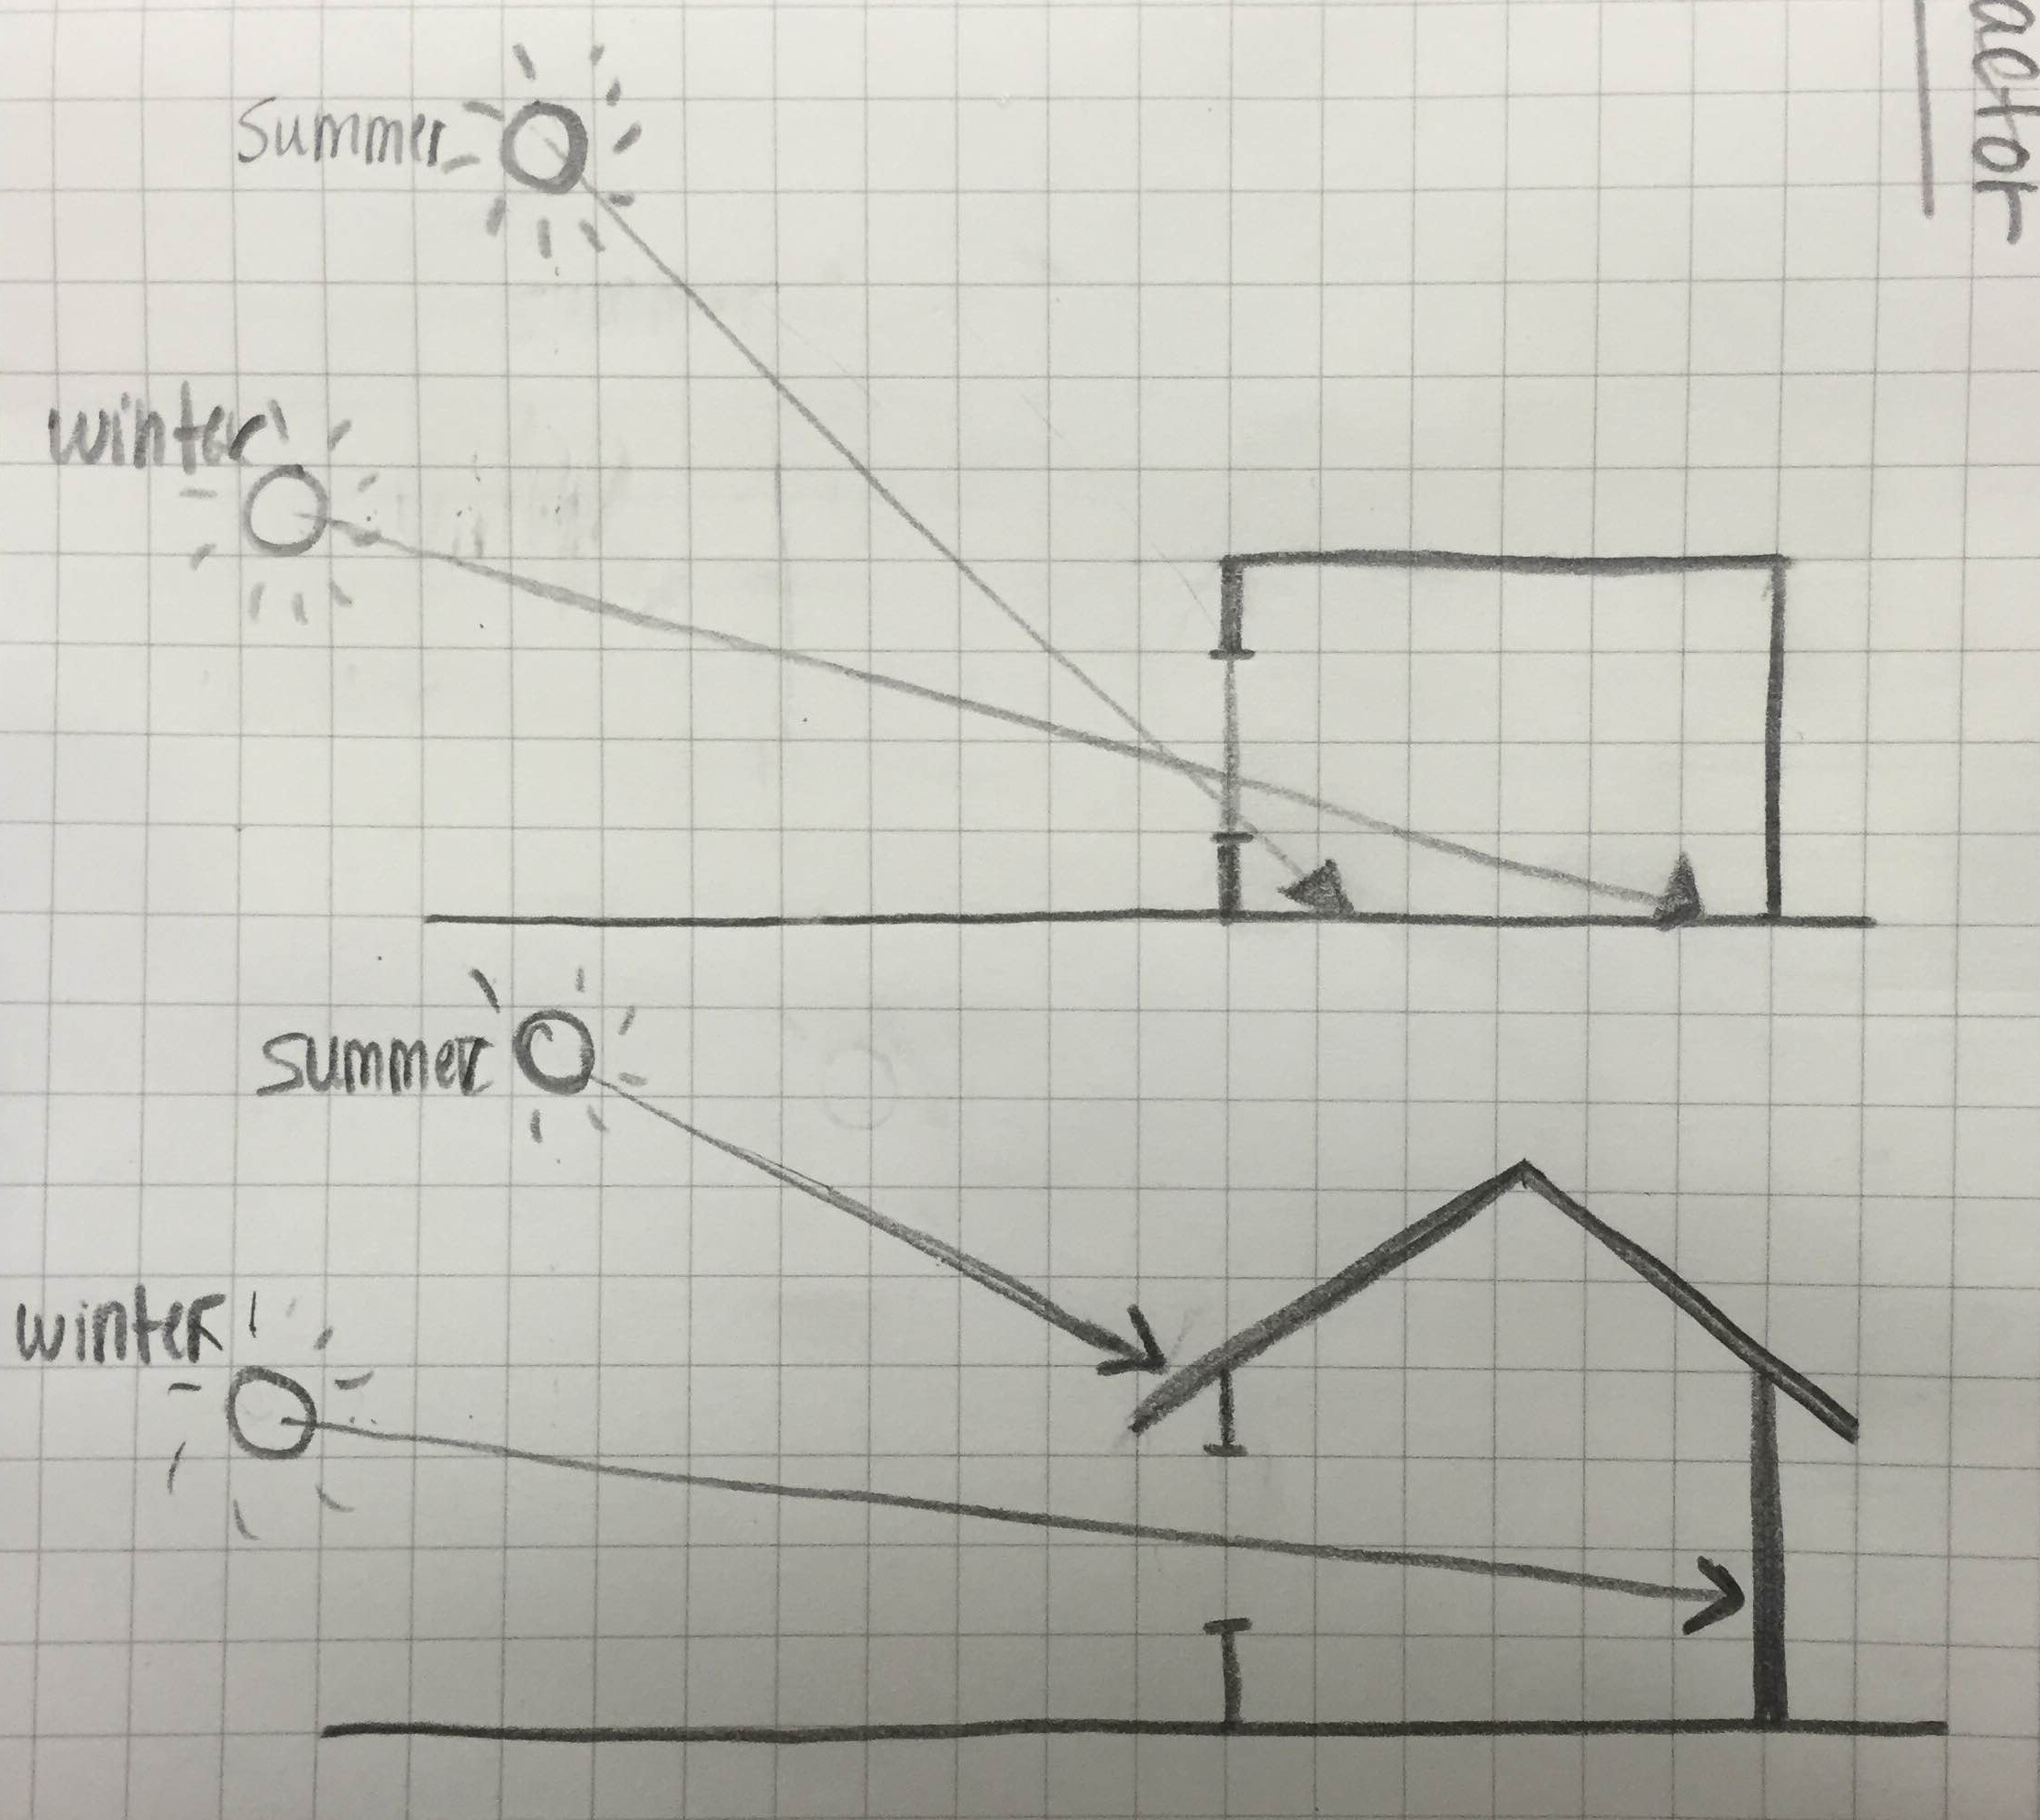
\includegraphics[width=0.5\textwidth]{summer_winter}
    \caption{Top: illustration to visualize the difference in light penetration during the winter and summer seasons. Bottom: a common daylighting technique is extending the roof to block light during the summer season, but not during the winter season.}
    \label{fig:summer_winter}
    \end{figure}

    Architects interested in sustainability, exploit this by extending the roof thus allowing daylight to enter during the winter and blocking direct daylight during the summer as shown in figure-\ref{fig:summer_winter}.
    Weather conditions also play an important role in the distribution and intensity of daylight. 
    During clear days, direct sunlight can enter a room and cause over illumination and glare.
    However during cloudy days, sunlight is diffused by clouds resulting in daylight that is more uniform and diffuse.
    Weather conditions also vary by location, for example in upstate New York, cloudy skies are common, however in Florida clear skies are more frequent.
    A Daylighting systems would be more efficient in locations with clearer skies then in locations where clear skies are uncommon.\\

    Overall, daylight varies due to many factors. It varies depending on temporal factors, room-specific design choices, and building-wide decisions. These numerous factors make the distribution of daylight in a architectural space non-trivial to predict. 
    These difficulties pose a real challenge in the designing of effective daylighting systems.

  \subsection{Adverse Daylighting Effects}

    As previously discussed, daylighting systems offer occupants a variety of benefits. However, poorly implemented daylighting systems can result in discomfort to occupants and increases in a building's energy demand.

    \paragraph{Occupant Discomfort}

    % Over and under illumination
    Human vision can be understood and compared to an image processing systems.
    We require strong contrast and ample illumination to be able to clearly view and process symbols.
    The performance of visual task, such as reading, varies depending on the illumination provided and clarity of the font.
    Under-illumination can make reading difficult and reduce worker productivity\cite{boyce}.
    Under illumination can occur in daylighting systems when daylight available is below a threshold to perform a specific visual task.
    The Occupational Safety and Health Administration (OSHA) set mandatory minimums on illuminations for common settings including offices, hallways, and warehouses to name a few.
    Offices for example require a minimum of 322 lux.
    % Extension: Add in how we compute lux
    Similarly, hallways and warehouses have lower minimums set because there is no need to focus on fine details\cite{OSHA}. \\

    Another visual discomfort that can occur from poor daylighting is glare.
    Glare is a reduction of contrast due a disproportionate amount of illumination from glare sources compared to illumination on a visual task.
    % Introduce the glare index
    Glare is hard to account for in the early design stages of architecture because glare is dependent on not only sources of illumination but also on viewpoint.
    Specifically, there are two main forms of glare -- disability glare and discomfort glare.\cite{Robbins}
    Disability glare occurs when a glare source is intense enough that it rendered the viewer momentary blind. 
    This kind of glare commonly occurs when driving at night and cars are passing in the opposite lane. 
    The strong light emitted from headlights would reduce the contrast of the road ahead and might result in momentary blindness.
    %
    Likewise, discomfort glare is similar to disability glare but much less dangerous. 
    Discomfort glare is also caused from bright glare sources, such as the Sun or light reflected from the Sun, that making visual task difficult to perform.
    Unlike disability glare, discomfort glare does not cause momentary blindness.  
    Prolonged exposure to discomfort glare when focusing on a visual task,however, significantly reduces both worker productivity and worker satisfaction\cite{boyce}. 
    Another visual discomfort, common in office environments, includes veiled reflection.
    Veiled reflections are the result of light reflecting off a surface directly into the eyes of the viewer. 
    For example reading an article from a glossy magazine in direct sunlight is challenging because at certain viewpoints the gloss on the page reflects light into your eyes reducing the contrast between both the black and white letters. 
    Veiled reflections, like glare, are difficult to predict because they are viewpoint dependent. \\

    Lastly, occupants sitting near windows can experience thermal discomfort at certain times of day.
    Daylight can be useful in warming up a space during the winter, however can also cause discomfort during the summer.
    Not only does unattained solar heat gain cause occupants discomfort, solar heat gain can also discomforts building owners.

    \paragraph{Economic Loss}
    
    Another possible adverse product of daylighting systems is unintended solar heat gain. Solar heat gain is the increase in temperature inside a space due to daylight. 
    If too many windows are installed in particular location, a room can experience unintended solar gains.
    To counter solar heat gain, cooling system must work at a higher load then usual resulting in increased energy usage.
    Furthermore, windows unless insulated well can result in heat loss during the winter.
    Rooms with many windows might let in a lot of daylight, but might also come at the cost of increased heating cost during the winter months.\\

    Lastly, occupant behavior can result in lose of investment capital for building owners.
    Occupants exposed to the visual discomforts of daylight can choose use window blinds to block daylight out entirely.
    If blinds are lowered then electrical lighting is used in place of daylight.
    The use of electrical lighting, given available daylight, results in reduced energy savings for the building owners.
    Moreover, daylighting systems are expensive to design and implement and as a result the initial cost is generally greater then using traditional electrical lighting.
    If occupants continuously choose electrical lighting over daylight, the break even point of the initial investment in a daylighting system is pushed back further -- essentially costing the building owner capital.
    Architects are then faced with the challenge of not only making visually pleasing lighting conditions, but also avoiding discomforts caused by daylight.

% This section needs to be written
\section{Daylighting In The Architectural Design Processes}

  % Introduction into subsections
  % Architects face the challenges of designing daylighting systems by using a variety of strategies and techniques.


  \paragraph{Schematic Design Phase} 
  Architects break apart the architectural design processes into 5 stages. 
  The earliest design stage is known as the schematic design phase.
  Prior to designing a building or space architects must first consult with clients and review project goals and specifications during this phase.
  Daylighting affects all stages of the architectural design process, and as a result, requires architects consideration early on.
  After understanding project specifications and project goals architects begin designing by sketching out general building forms and mass. These are rough sketches, however these sketches can be studied to analyze the quality of a design. Shapes and forms of building are usually tackled in a creative and iterative fashion. Sketches still remain widely used during this stage. With enough practice conveying 3D visual concepts through rough sketches is quick and efficient.
  % Figure of what these sketches look like
  Similarly, other mediums can be used to study a design during the schematic design phase such as physical scale models.
  Lastly,the relationships between rooms and spaces are also defined during this phase, including the intended purpose of specific spaces.

  \paragraph{Design Development Phase} 

  Firstly, architects use a set of rules and helpful visuals during the first stage of the architecture design process to guide the . 
  Secondly, once the initial form and design of a project is selected there is another set of tools and devices that help designers develop daylighting system.
  By and large, most challenges in the design of daylighting systems have seen the development of strategies and techniques aimed at alleviating the difficulty posed by designing with daylight.\\

  \subsection{Schematic Design Phase}
    % Intro into the three points we are going to make
    % What is the schematic design phase
    Architects interested in sustainability have many strategies to manage the complexity of creating daylighting.
    Firstly, there are numerous rules-of-thumb aimed to guide the conceptual design of a building to make the best use of daylight.
    Secondly, previous experiences play a significant role in decision making when designing daylighting systems. Lastly, architects during the early design stages still rely on brief analysis of hand drawn sketches to predict lighting behavior in a space. In summary, there are many tools and techniques designs can leverage when building a daylighting system.\\

    \paragraph{Rules-of-Thumb}
    Architects use general rules-of-thumb during the earliest stage of the design process. 
    During the schematic design phase, architects develop the general form, shape, and mass of an architectural space.
    Because the design of a space is an iterative process, where alterations are made until all requirements set by the client are set\cite{Suwa}, any techniques or strategies used to guide the design of daylighting systems need be quick and easy-to-use. Rules-of-thumb are used in conjunction with sketches guide the design process.
    Recent work at the Lighting Research Center validated some common rules-of-thumb architects have used in the design of daylighting systems\cite{Leslie}.
    One such rule validated is the elongation buildings on the east-west axis.
    In addition, another rule validated is the placement of windows high up a wall.
    Having windows high up allows for deeper penetration of daylight into a space.
    Similarly, direct sunlight is best diffused by using shading devices or by bouncing off interior surfaces.
    Moreover, moving visual task closer to windows takes full advantage of daylight.
    However, moving workstations closer to windows increases the risk of glare. A common rule-of-thumb to mitigate is move workstations perpendicular to windows.
    Overall, there are plenty of rules-of-thumb involved in the design of early daylight system.\\

    \paragraph{Experience}
    % Paraphrase: Determining the amount of aperture in the very beginning of schematic design is most often based on a designer’s experience or on rules of thumb


    \paragraph{Visualizations on Hand Drawn Sketches}

    Ideas are though up and written in the form of pencil sketches.
    Architects use sketches to facilitate problem solving. 
    After sketching a idea, architects and look back on their sketch and try to find problems and improve upon their initial sketch.
    Sketches are a great medium because with practice, sketching becomes an easy and fast medium to represent 3D geometries\cite{Suwa}.

  \subsection{Design Development Phase}
    % Intro into the two points we are going to make

    \paragraph{Virtual 3D Models}
    \paragraph{Physical Scale 3D Models}


    %%%%%%%%%%%%%%%%%%%%%%%%%%%%%%%%%%%%%%%%%%%%%%%%%%%%%%%%%%%%%%%%%%%
%                                                                 %
%                            CHAPTER TWO                          %
%                                                                 %
%%%%%%%%%%%%%%%%%%%%%%%%%%%%%%%%%%%%%%%%%%%%%%%%%%%%%%%%%%%%%%%%%%%
\chapter{RELATED WORKS} \label{sec:introduction}
% Introduction into the 3 topics below we are about to cover
	% Sentence Hook
	% Sentence 1: Virtual Heliodon
	% Sentence 2: Daylighting Software
	% Sentence 3: Crowd Sourcing User Study
	% Sentence Recap

\section{Virtual Heliodon}
    % Introduction explaining that my work is a extensions to this work
    % SAR sentence
    % Sketch Interface sentence
    % Recap

	\subsection{Daylighting Design with A Spacial Augmented Reality}
		% Introductory Sentence ( Don't know what to say exactly)
		% The augmented reality with projectors
		% LSVO + Daylighting
		% Recap why 

		\paragraph{Augmented Reality with Projectors}
			% mention projectors and coverage
				% slight mention of problems with coverage
			% collaborative space
			% people tokens
			% immerse space + engaging

		\paragraph{LSVO + Daylighting Simulation}
			% mention to radiance
			% mention to why we choose lsvo > radiance
				% speed
				% good results given a small time window
			% mention to how this works with photon mapping and optix
				% mention how it is a gpu thing

	\subsection{Floor Plan Design with A Physical Sketching Interface}
		% Introductory Sentence ( Don't know what to say exactly)
		% 3D modeling types 
		% How we are using sketching borrowed from virtual Heliodon

		\paragraph{3D Modeling}
			% Talk about what parametric modeling is
				% mention HEED
				% mention eQuest
			% Talk about what geometric modeling is
				% Mention sketchup
				% Mention autodesk

			% Talk about sketching modeling
			% Talk about how Barb did this shortly
			% Mention how we use this

		\paragraph{Related Sketching Interfaces}
			% Similar to lightsketch
			% Similar to VR sketchpad proj
			% Similar to erics ref paper

\section{Daylighting Software}
	% Compare Velux
	% Compare Project Versai
	% Compare LightSketch
	% Compare design builder
	% Compare plug-ins
		% Compare ecotect
		% Compare ladybug
	% Wrap things up in this sentence

\section{Crowd sourcing User Studies}
	% Mention crowd sourcing a useful research tool for validations of software.

	% Papers to reference: Crowd sourcing User Studies w/ Mechanical Turk
		% Economics of user studies
			% Time constants
			% low-cost & timely
			% collecting input from only a small set of participants is programmatic in many design situations(even large one) are easily caught with small number of participants

	% Web Credibility Research: A Method for Online Experiments and Early Study Results
		% TODO Information:
			% things you can do to make a website seem credible
			% reduce ads and increase attainability
			% this study shows that online studies are much faster, and much larger then normal studies
			% you can a global demographic

	% Testing Web Sites: Five Users Is Nowhere Near Enough 
		% TODO information:
		% 5 users catch 35% of the problems for websites ( was assumed to 85%)
		% rethinking of our usability engineering testing
		% if we really want to make a useful tools feedback frequently is important

	% Crowd-Sourced Peer Feedback (CPF) for Learning Community Engagement: Results and Reflections from a Pilot Study
		% TODO information:
		% CPF increase engagement, motivation, and learning
		% we might want to use this to teach daylighting
		% we get engaged,motivated, and learn from feedback, so it would good for researchers.

	% Papers to ref: Cookies of Cobblers?
		% Crowds can be leverages to partake in a creative iterative design processes.
		% Maybe we can get crowd sourced arch sketches
		% Enhanced creativity

	% Papers to ref: Real-time Drawing Assistance through Crowd sourcing
		% This paper uses data collected from users to find out what are the important lines drawn on face 
		% closing the loop, the game itself serves as a platform for large-scale evaluation of the effectiveness of our stroke correction algorithm.


%%%%%%%%%%%%%%%%%%%%%%%%%%%%%%%%%%%%%%%%%%%%%%%%%%%%%%%%%%%%%%%%%%%
%                                                                 %
%                            SCRAP YARD                           %
%                                                                 %
%%%%%%%%%%%%%%%%%%%%%%%%%%%%%%%%%%%%%%%%%%%%%%%%%%%%%%%%%%%%%%%%%%%
	% The need for daylighting analysis earlier in the architectural design process, drives the development of tools that generate timely results at affordable levels of effort.
	% In order to perform daylighting analysis, these tools must either import or generate 3D models of architectural spaces.
	% Some tools come packaged with their own parametric or geometric modeling capabilities, however, other tools are available as plug-ins for existing geometric modeling software.
	% Moreover, there are handful of daylighting analysis tools that use sketching inspired interfaces for generating 3D models.
	% All of the analysis tools mentioned below face similar challenges.
	% These tools attempt to provide a means to perform daylighting analysis earlier in the architectural design process.

	% \section{Early Design Phase Parametric-Modeling Daylighting Tools}

	% 	Some early design tools such as HEED and eQUEST allow users to defined architectural spaces with parametric-modeling interfaces. 
	% 	Parametric modeling, as seen in HEED and eQUEST, is the creation of architectural models by defining a set finite parameters.
	% 	These parameters, such as room dimensions, define an architectural space.
	% 	In order to manage the large number of parameters required to analyze energy consumption of a space, both HEED and eQuest use wizards to guide users along the complex processes of defining an architectural space.

	% 	Remarkably, for eQUEST 41 pages of parameters must be defined before conducting analysis on a space given a full 3D model.
	% 	However, parametric modeling doesn't offer much flexibility in design of models.
	% 	HEED and eQUEST are both early design tools that provide users with energy design analytical tools -- including daylighting.
	% 	But because the tools cannot create 
	% 	These tools provide only quantitative data to architects, and do not produce rendering.

	% 	%\subsection{HEED}

	% 	%\subsection{eQUEST}

	% \section{Early Desing Phase Geometric-Modeling Daylighting Tools}
	% 	%\subsection{Sketchup with Lightsolve}
	% 	%\subsection{Autodesk with Ecotect}
	% 	%\subsection{Rhino with Ladybug}
	% 	%\subsection{Velux}
	% 	%\subsection{Daylight-1-2-3}

	% \section{Early Design Phase Sketch-Modeling Daylighting Tools}
	% 	%\subsection{Light Sketch}
	% 	%\subsection{Virtual Heliodon}

    \chapter{Feature Design} \label{sec:feature}

% Introduction into sections
\section{System Overview}
This chapter covers in detail what OASIS is as an architectural sketching interface and what our goals for OASIS are. In addition to discussing what our objective for OASIS is, I also discuss OASIS in relation to the Virtual Heliodon. We additionally explain the importance user interface plays in software and tools like OASIS. Moreover, we cover the specific design choices made in the sketching of walls and windows, furniture placement, and other related sketching operations; alternatives to sketching operations  currently used in OASIS are also considered in this chapter.
Afterward, I cover the types of 3D models available to users on OASIS in the \textit{Generate a 3D model} page and \textit{Analyze Simulation} page.General web application design choices, not pertaining to the sketching interface and model viewer, are also covered. We also elaborate on problems encountered during the design of OASIS and the solutions to those problems. Some implementation details are discussed at the end of the chapter. Overall, this chapter covers my contributions to the design of OASIS.


\paragraph{What is OASIS}
% What is OASIS
% What is your objective with oasis
The online architectural sketching interface for simulations (OASIS) is intended to be a  general early design tool for both novices and architects. OASIS provides a platform independent sketching interface that generates closed 3D triangle meshes with optimal properties for simulations. Currently, OASIS only supports daylighting visualizations; however, OASIS can be extended to support other simulations that make use of closed triangle meshes, including acoustic and thermal simulations. The main advantage OASIS offers users is an novel interface that does not require detailed geometric modeling for the creation of 3D triangle meshes and an interface to analyze simulation results. An additional advantage of using OASIS is the client-server architecture that allows users to be able to run computationally expensive simulations at interactive rates regardless of their machine specifications.

\paragraph{Virtual Heliodon Pipeline}
% <Pipeline of the Virtual Heliodon>
Both OASIS and the Virtual Heliodon provide a novel solution to the challenge of daylighting analysis during the early stage of architectural design.
In addition to sharing the same objectives both OASIS and the Virtual Heliodon utilize the physical sketch interpretation algorithm and the daylight rendering engine.
As a result it can be difficult to see where these two systems vary.
In order to understand the contributions I made to OASIS we must briefly cover the system pipeline of the Virtual Heliodon.
\begin{figure}[!ht]
\centering
\caption[The Virtual Heliodon's simplified pipeline.]{Virtual Heliodon's simplified pipeline. A and B are locations in the pipeline that require an experienced operator to perform technical actives on the Virtual Heliodon. }
\label{fig:pipeline_vh}
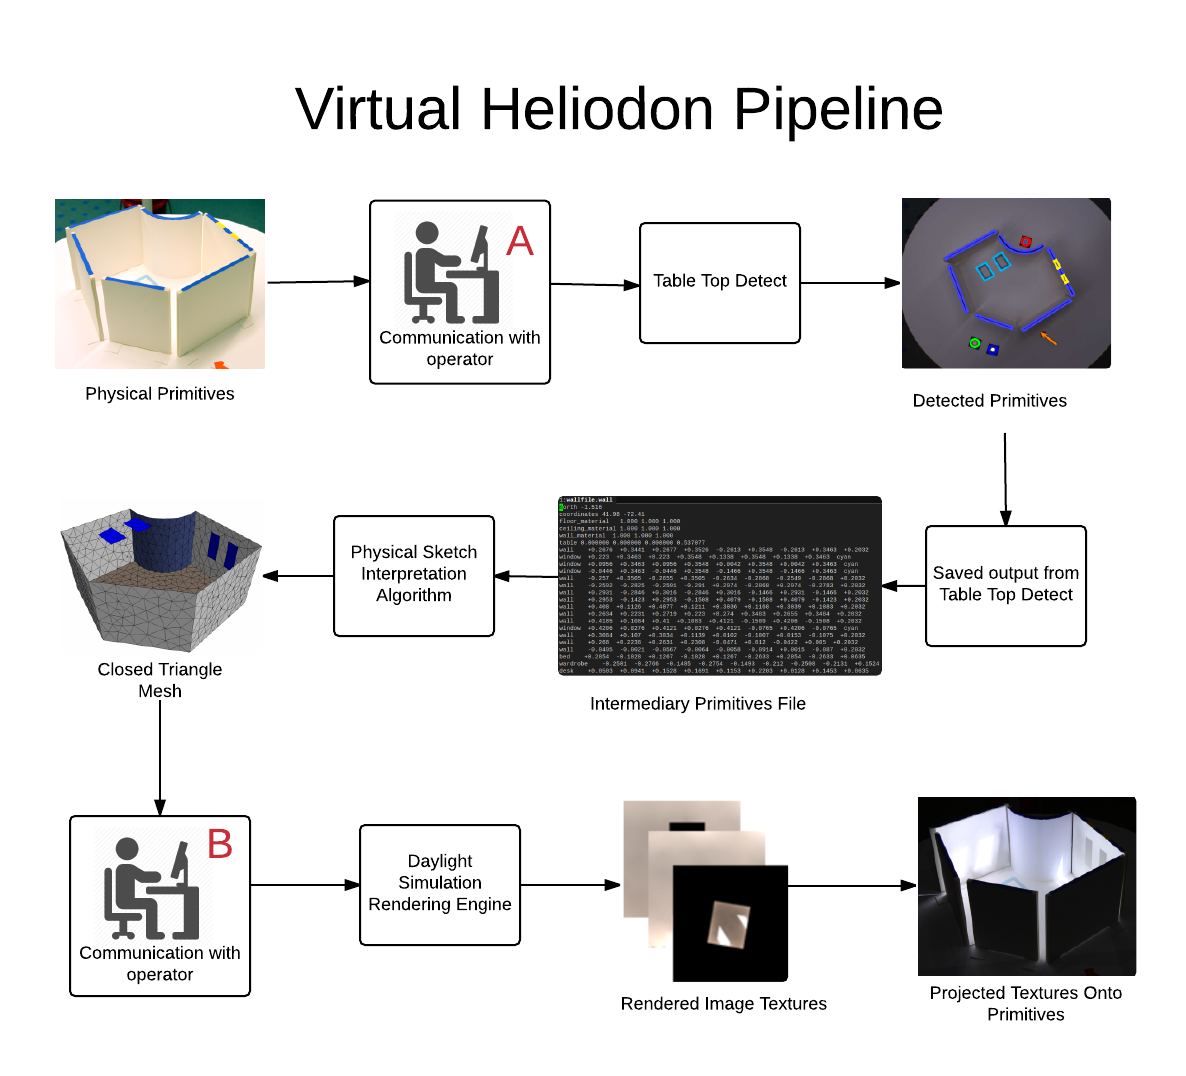
\includegraphics[width=1.0\textwidth]{pipeline_vh}
\end{figure}
The Virtual Heliodon's system pipeline is illustrated in Figure-\ref{fig:pipeline_vh}.
To begin, the Virtual Heliodon features a novel tangible user interface for the creation of architectural spaces.
Users define architectural spaces by manipulating physical foam primitives with their hands.
After users are satisfied with their architectural space they can either use a wireless clicker or communicate to the operator to run the \textit{table top detect} process and continue to generate a closed triangle mesh from their physical sketches; Communication with the operator to run the \textit{table top detect} process is noted in Figure-\ref{fig:pipeline_vh}A.
The \textit{table top detect} processes is a simple computer vision program that takes an overhead image of the foam primitives and detects where those primitives are in an image.
The coordinates of where those primitives are in an image are stored in an intermediate primitives file. The intermediate primitives file is used as input for the physical sketch interpretation algorithm. As mentioned previously, the physical sketch interpretation algorithm generates a closed watertight triangle mesh.
Currently, there exist no user interface for the generation of daylight visualizations.
Instead, an operator familiar with the system is required to generate visualizations for users, as shown in Figure-\ref{fig:pipeline_vh}B.
After the generation of  a watertight 3D mesh, users communicate to the operator the time and date they would like visualized. 
Depending on the time,date, and user visualization requested the operator would manually modify existing scripts to generate those visualizations on the Virtual Heliodon.
These scripts would include invoking the daylight rendering engine to generate image textures to be projected onto users' physical sketches.
In other words, the Virtual Heliodon does not offer much autonomy and requires an operator to both explain how to use the tangible user interface and constantly communicate with users to operate the Virtual Heliodon.
% </Pipeline of the Virtual Heliodon>


\paragraph{OASIS Pipeline}
OASIS is an alternative interface to the Virtual Heliodon. 
The system pipeline in Figure-\ref{fig:new_pipeline} illustrates the components involved in OASIS.
In addition, Figure-\ref{fig:new_pipeline} emphasizes all portions of OASIS that I directly contributed to.
To begin, users on OASIS generate 2D sketches consisting of lines that represent wall and windows and objects that represent furniture items.
The physical sketch interpretation algorithm that the Virtual Heliodon uses to generate watertight 3D meshes for simulations require sketches be given as a collection of model primitives. 
Therefore, before being able to invoke the physical sketch interpretation algorithm, OASIS generates the intermediate primitives file.
Model primitives are stored in an intermediate primitives file where each line describes a wall,window, or furniture item in a sketch.
\begin{figure}[!ht]
\centering
\caption[Diagram of OASIS pipeline.]{OASIS pipeline diagram with the author's contributions noted in blue.}
\label{fig:new_pipeline}
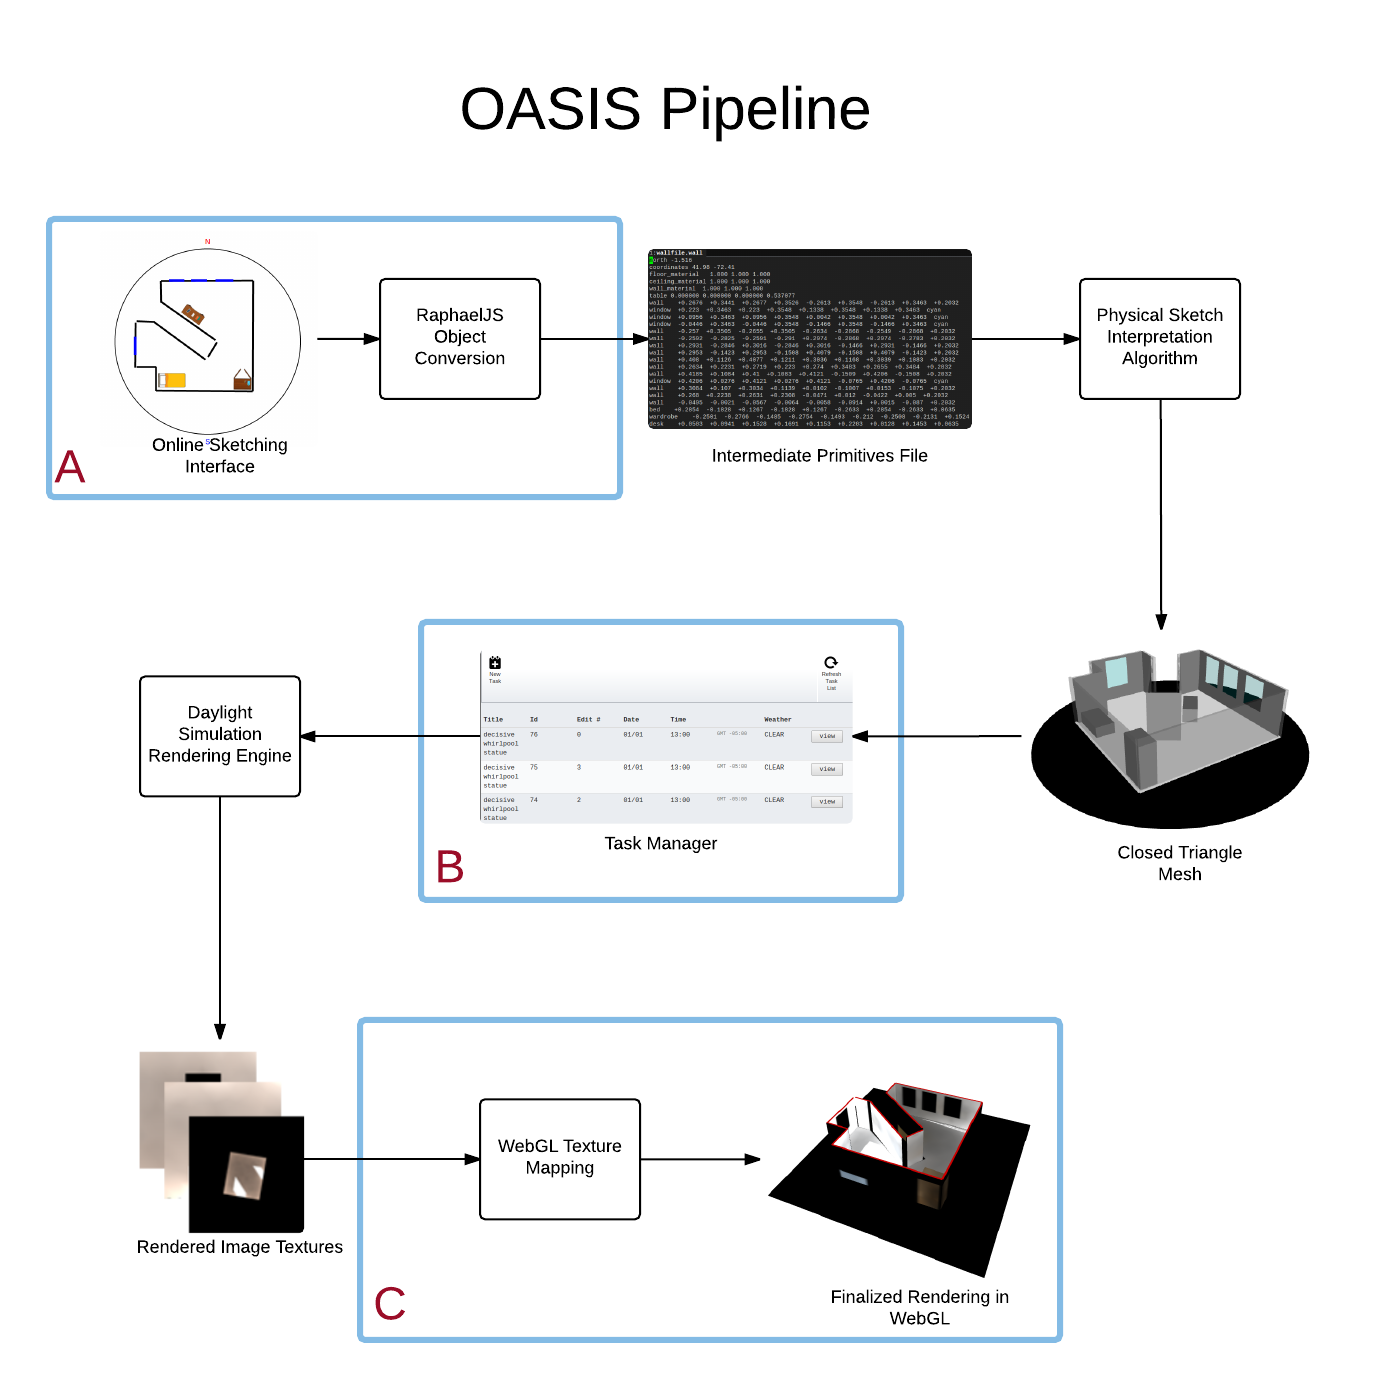
\includegraphics[width=1.0\textwidth]{new_pipeline}
\end{figure}
As mentioned previously, in the Virtual Heliodon the intermediate primitives file is created by a simple computer vision algorithm that detects walls, windows, and tokens through colored markers placed on the top of physical primitives.
Since the sketching interface is purely in-software, I can directly create this intermediate primitives file without need of a computer vision algorithm to detect primitives.
Interestingly, OASIS avoids a few limitations of the Virtual Heliodon by bypassing the need to detect physical primitives. 
OASIS can support a wider vocabulary of primitives because it is not bound to the detection of colored tokens.
Additionally, at certain angles parallel wall primitives in close proximity to each other on the Virtual Heliodon could result in the occlusion of primitives in the overhead image. 
Since OASIS is an in-software solution, this problem is avoided as the position of all primitives is always known.
Figure-\ref{fig:new_pipeline}A illustrates where OASIS generates the intermediate primitives file in our system pipeline.
Given the intermediate primitives file the physical sketch interpretation algorithm outputs a closed triangle mesh that the user can view in the \textit{Generate 3D Model} page.
The user can create a daylight simulation request in the \textit{Create Daylighting Simulation} page, given confirmation that a 3D generated model matches the user's intention.
This portion of the system pipeline is illustrated in Figure-\ref{fig:new_pipeline}B.
After the submission of a daylight simulation request, I use the daylight simulation rendering engine to produce texture images.
These texture images capture global illumination from a daylight simulation in a viewpoint independent manner.
On the \textit{Analyze Daylighting} page, I map these texture images onto the 3D mesh to display a daylight rendering of the user's generated model.
Figure-\ref{fig:new_pipeline}C illustrates where texture mapping occurs in the system pipeline.
In brief, our pipeline shows that OASIS is an alternative autonomous interface to the physical sketch interpretation algorithm and daylight rendering engine used in the Virtual Heliodon.



\paragraph{Basic Navigation and Pages}

OASIS consist of six pages that users can navigate between linearly and non-linearly; these pages are illustrated in Figure-\ref{fig:overview}.
Each of these pages, with the exception of the login/register page, are accessible through respective tabs located at the top most portion of the page.
Each respective page, allows users to interact with different portions of our system pipeline.
For beginners it is recommended that pages are followed linearly from step 1 to step 5.
Figure-\ref{fig:overview}A illustrates the first page users encounter when opening our web application.
The \textit{Login/Registration} page is designed to be as minimal as possible to encourage users to register and try out OASIS.

\begin{figure}[!ht]
\centering
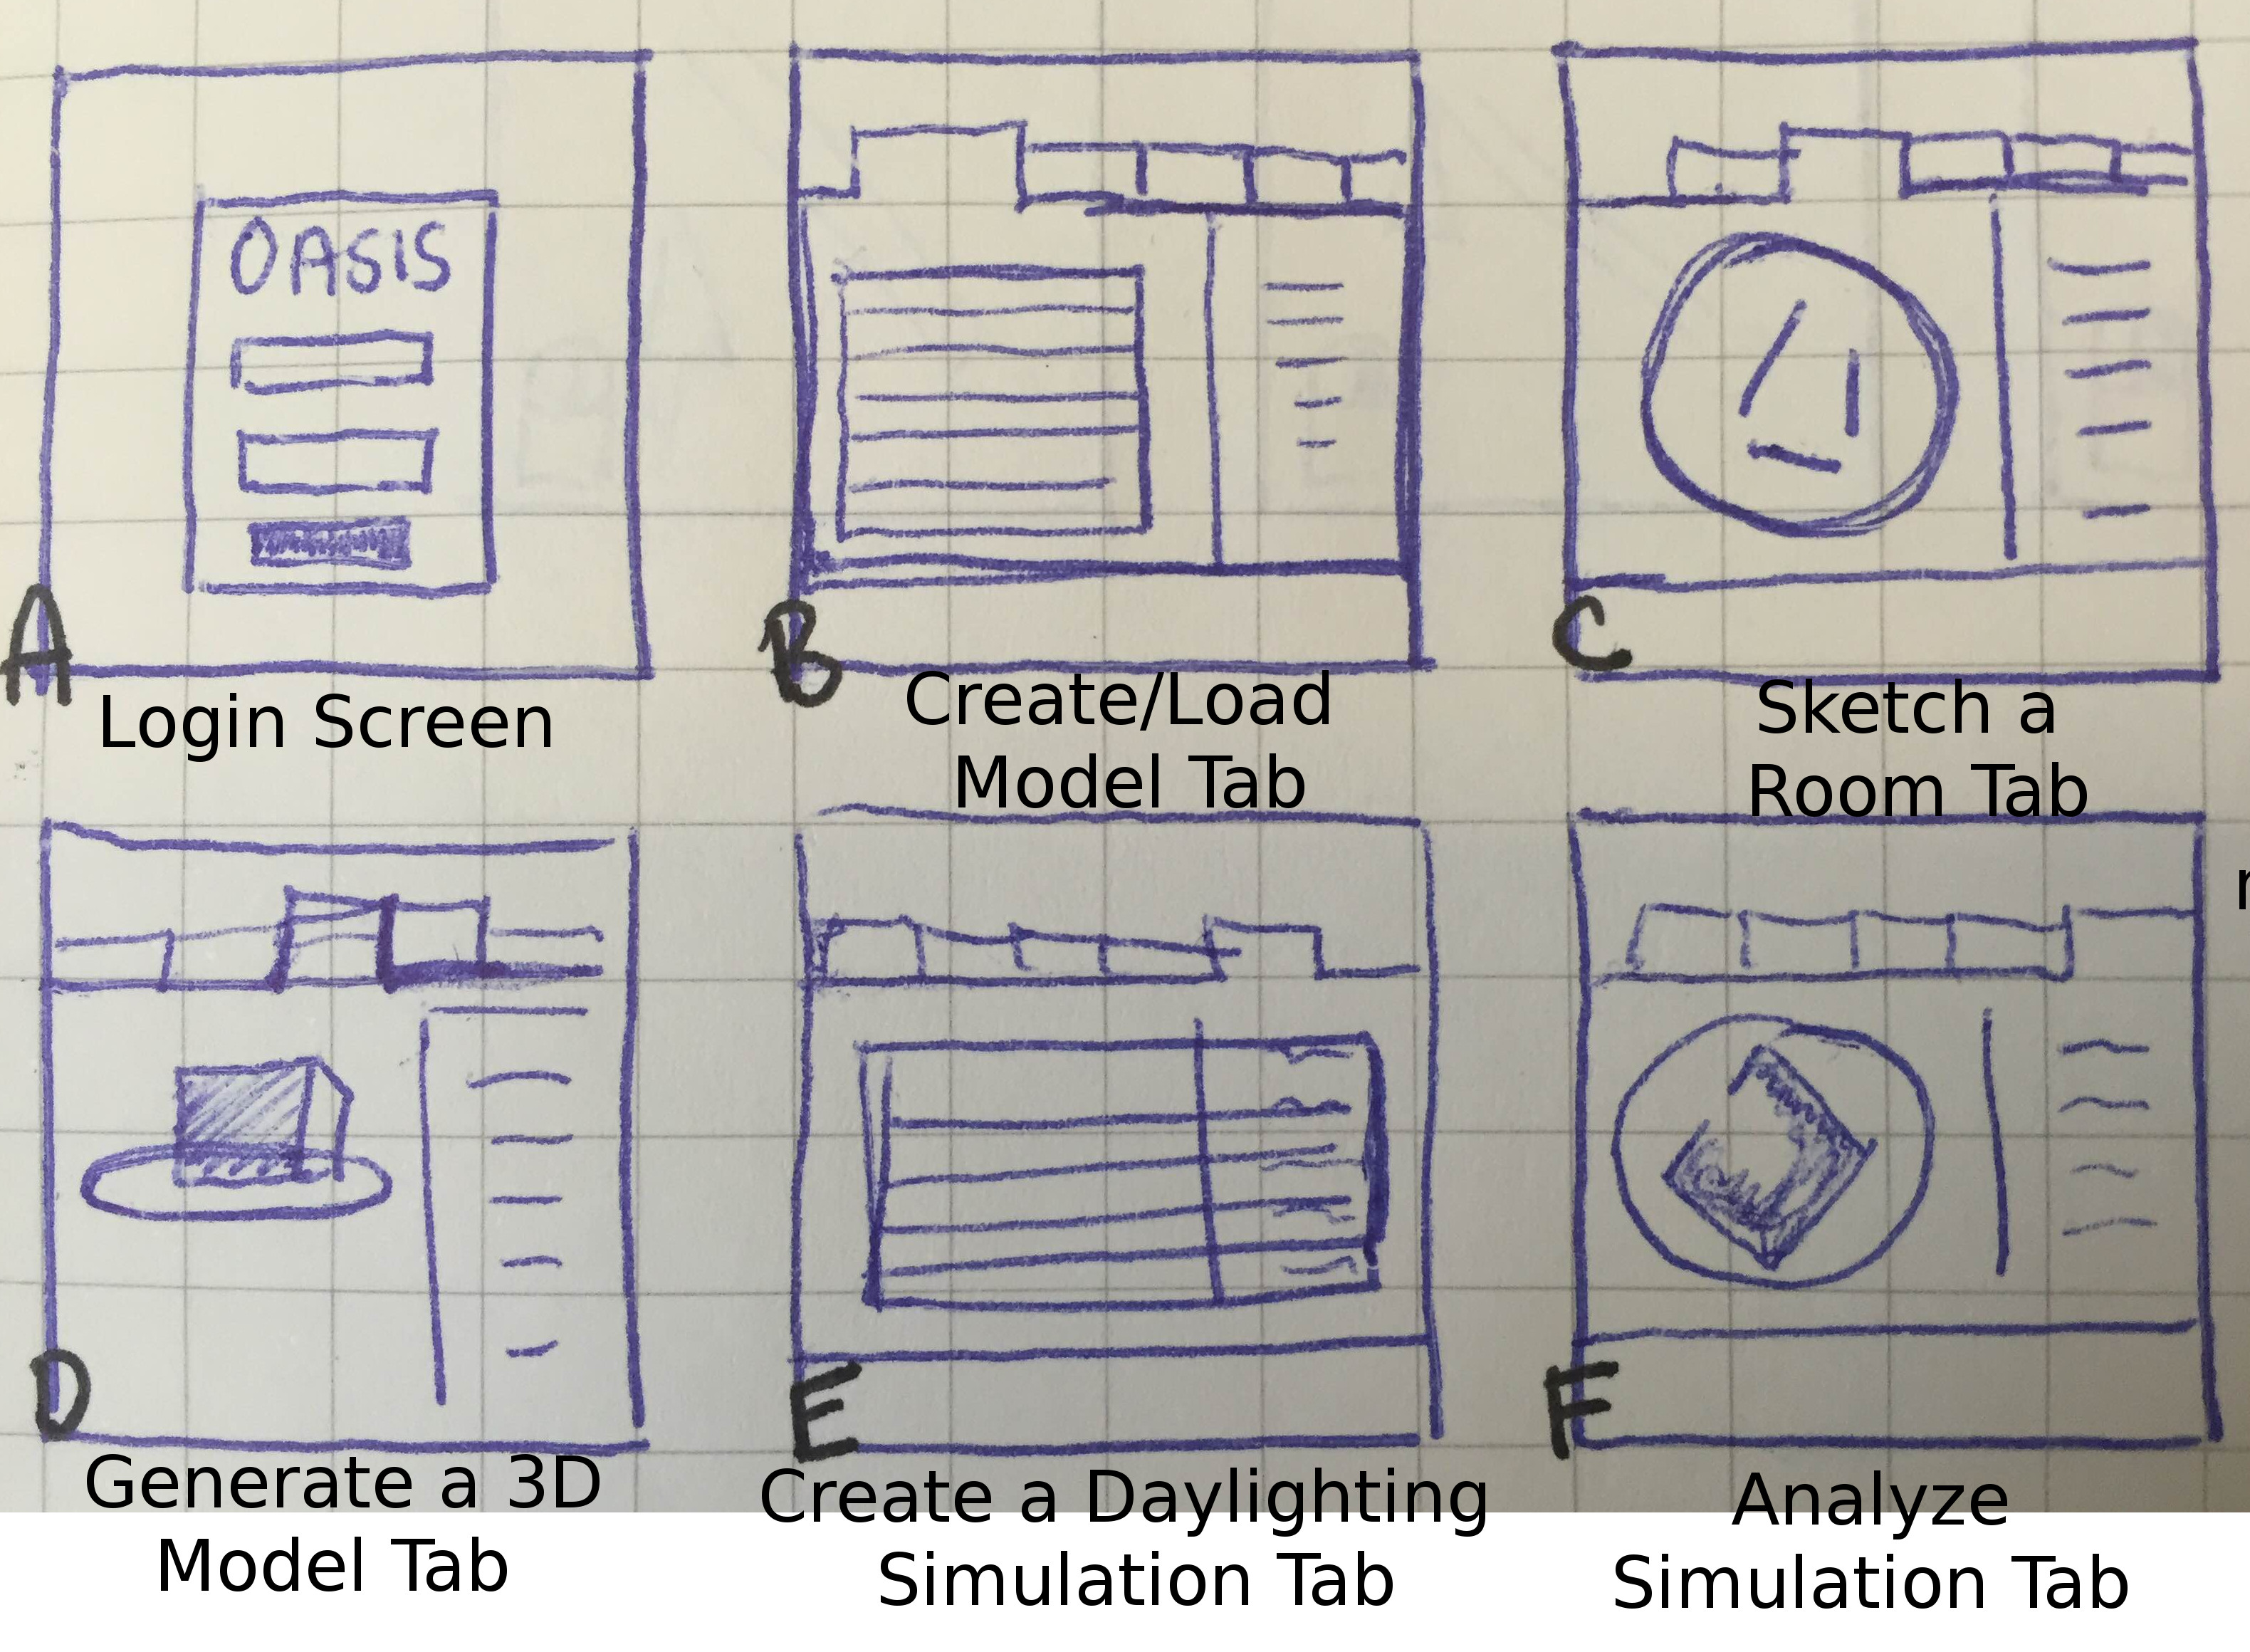
\includegraphics[width=0.8\textwidth]{overview}
\caption{This is an overview of the pages on OASIS.}
\label{fig:overview}
\end{figure}

After a successful login or registration, the first page users are directed to is the \textit{Create/Load Model} page.
The \textit{Create/Load Model} page contains a selectable list of users' previously created sketches and the option to create new sketches.
The \textit{Create/Load Model} page is illustrated in Figure-\ref{fig:overview}B.
Assuming users follow the pipeline linearly, users would either load previously created models or start new models.
Either action would result in a redirection to the \textit{Sketch a Room} page, shown in Figure-\ref{fig:overview}C.
The \textit{Sketch a Room} page contains the architectural sketching interface.
After the user is satisfied with their sketch they can proceed to the \textit{Generate 3D Model} page.
Visiting the \textit{Generate 3D Model} page will invoke the generation of an intermediate primitives file; afterward OASIS passes the intermediate primitives file to the physical sketch interpretation algorithm. This creates a 3D watertight triangle mesh object that is displayed on the \textit{Generate 3D Model} page.
Figure-\ref{fig:overview}D illustrates the \textit{Generate 3D Model} page.
Depending on the 3D watertight triangle mesh object created the user can either confirm their intention was met and navigate to the \textit{Create Daylighting Simulation} page or navigate back to the \textit{Sketch a Room} page to make alterations.
On the \textit{Create Daylighting Simulation} page the user can either create new daylight renderings or view previously created renderings, as seen in Figure-\ref{fig:overview}E.
How to create a rendering is depicted in detail in Figure-\ref{task}.
After the creation of a rendering users can then click on the \textit{view} button associated with the rendering of interest.
Clicking the \textit{view} button will redirect users to the \textit{Analyze Simulation} page.
The \textit{Analyze Simulation} page will display a daylight rendering that users can interact with for analysis.
Figure-\ref{fig:overview}F illustrates the \textit{Analyze Simulation} page.
The \textit{Analyze Simulation} page will also host a variety of daylight visualizations that users can toggle between to perform both qualitative and quantitative daylight analysis.
All in all, we hope that OASIS has a small learning curve and allows users to quickly preform daylight analysis with the least cost of effort.


\begin{figure}[!ht]
\centering
\caption[How to create a request for daylighting simulations.]{How to create a request for daylighting simulations. 
A) The user must first click on the \textit{create new task} button.
B) The user must then define daylighting parameters such as date and time. Once complete the user may click the submit button to submit their request.
C) The user's task is added to the table and the status of the task is displayed.
D) Once the task is complete the user can click on the view button
E) The user will be redirected to the \textit{Analyze Simulation} tab to view their rendering.
}
\label{fig:task}
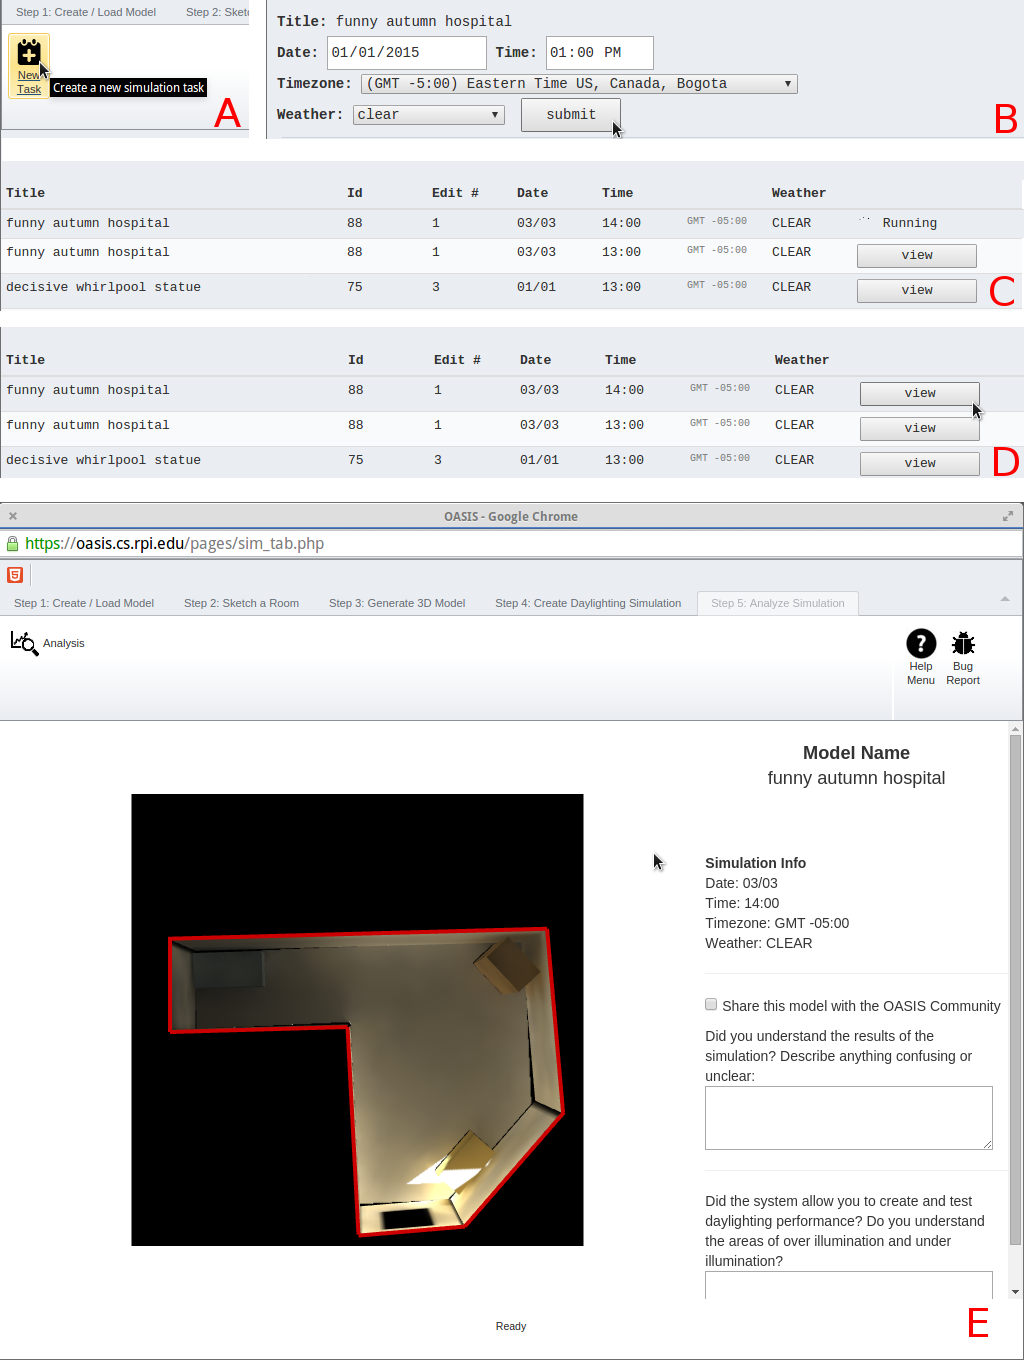
\includegraphics[width=1\textwidth]{task}
\end{figure}

\clearpage

\paragraph{Importance of UI}\label{ui_importance}
A previous survey discovered that on average 48\% of written code for a given application is made up of user interface implementation\cite{Myers1992}.
The same survey also noticed that 50\% of time spend coding an application is devoted to implementing the user interface\cite{Myers1992}.
User interface design is important to the success and usability of any piece of software.
Bottlenecks in a tool's user interface can result in user frustration and a reduction in users' productivity.
% <Discussion of Current UI?>
As a result OASIS is intended to provide an autonomous easy-to-use interface for interacting with the physical sketch interpretation algorithm and daylight rendering engine.
Notably, we define easy-to-use  as a general term that refers to the lack of formal training required to use a tool.
As discussed previously, the interface in the Virtual Heliodon requires an experienced operator at all times.
It is important to note that there has been attempts to give users control over the Virtual Heliodon including programming a remote clicker to trigger the \textit{table top detection} process.
However, there is currently no user interface for choosing visualizations to display and define the parameters required by those visualizations.
The Virtual Heliodon, just like OASIS, aims to be an easy-to-use interface for not only the design of architectural spaces but also the generation of helpful visualizations.
Requiring an operator with programming experience and background knowledge on the Virtual Heliodon may hinder users' creative iterative design process.
% < Closing statement of UI>
By and large, the user interface can make or break an application and as a result we stress the importance of interfaces that are both autonomous and easy-to-use.

\section{Sketching Interface Design}

\subsection{Sketching Walls and Windows}
% Why is sketching walls/win important
The boundaries that define an architectural space are composed of walls and other dividing objects.
The  boundaries of an architectural space must be well defined, in order to produce a 3D watertight triangle mesh.
The physical sketch interpretation algorithm differentiates the interior and exterior of a sketch in the process of generating a 3D watertight triangle mesh.
Consequently, the physical sketch interpretation algorithm requires walls to perform this differentiation\cite{cutler2010interpreting}.
The interface that allows users to define where walls in windows are placed in a sketch is important to the generation of 3D watertight triangle meshes and the overall usability of OASIS.\\
 
% Discussion about what we do
OASIS mimics physical drawing via a click-draw-release procedure.
The click-draw-release procedure is illustrated in Figure-\ref{fig:wall_win}.
In order to draw walls users must first toggle the \textit{wall drawing} mode on OASIS;
Toggling the \textit{wall drawing} mode is done by clicking on the \textit{wall} button located at the top of the \textit{Sketch a Room} page, as illustrated in Figure-\ref{fig:wall_win}A.
% Checkpoint
Then, as Figure-\ref{fig:wall_win}B and C illustrate, by holding the left mouse button and dragging anywhere on the canvas the user is shown a preview of where a wall will be drawn.
By releasing the left mouse button, the wall preview will be replaced by a drawn line, representing a wall, as Figure-\ref{fig:wall_win}D depicts.
Once a wall is drawn further editing is not allowed.
To keep with the spirit of sketching, windows are also placed into a sketch by being drawn similarly to walls, as shown in Figure-\ref{fig:wall_win}E through G.
However, unlike walls, windows need to be associated with a wall.
As a result a window needs to be drawn on or near a wall.
In the interest of the user, windows do not need to be drawn exactly on walls.
A window when drawn near a wall sharing a similar angle will automatically target and snap onto that wall, as illustrated in Figure-\ref{fig:wall_win}H.
This snapping feature makes drawing windows less reliant on users' precision with their input device, but rather focuses on users' intention. \\

% Discussion about alternatives(old method)
An alternative interface that was implemented but not used, allows users to create walls and windows via a drag-and-drop procedure;
The drag-and-drop procedure is illustrated in figure-\ref{fig:oldvh}D through F.
Users could then further manipulate walls and windows by both rotating and scaling them through the use of FreeTransform handles. 
FreeTransform handles are three white circular handles that are overlaid onto walls and windows.
One circle appears at the center and another circle is placed some distance away from the wall or window, as illustrated in Figure-\ref{fig:oldvh}F.
The circular handle in the center can be used to translate the primitive to anywhere on the canvas.
The circular handle off the side of the primitive is used to both scale and rotate the primitive to a desired length and angle.
Moreover, Figure-\ref{fig:oldvh} illustrates the parallels between how users place walls  into a scene in both the Virtual Heliodon and via the drag-and-drop procedure.
Both Figure-\ref{fig:oldvh}A and D illustrate how users have to select a primitive from a collection of primitives in both the Virtual Heliodon and via the drag-and-drop procedure.
Figure-\ref{fig:oldvh}B and E show how users have to place selected primitives on a surface, such as the physical table top or the online interface's canvas.
Figure-\ref{fig:oldvh}C and F demonstrate how users adjust either physical primates through physical interaction or the manipulation of FreeTransform handles.
However, despite mimicking how primitives were placed in the Virtual Heliodon, our eventual goal with OASIS is to pursue the most intuitive interface for drawing walls and windows.
The  drag-and-drop procedure focused on mimicking user interaction on the tangible user interface.
Overall, further testing, such as A/B testing, would be required before any conclusions can be drawn as to which interface is more intuitive.\\

\begin{figure}[!ht]
\centering
\caption
[Similarities between the drag-and-drop procedure and the Virtual Heliodon's Tangible User Interface.]{
 A) Users select a physical primitive from a collection of primitives. 
 B) Users place primitive on the table top. 
 C) Users adjust the primitive as desired. 
 D) Users select a primitive from a tray on the bottom of the interface. 
 E) Users drag that item onto the table. 
 F) Users use FreeTransform handles to scale and rotate the primitive as desired.
}
\label{fig:oldvh}
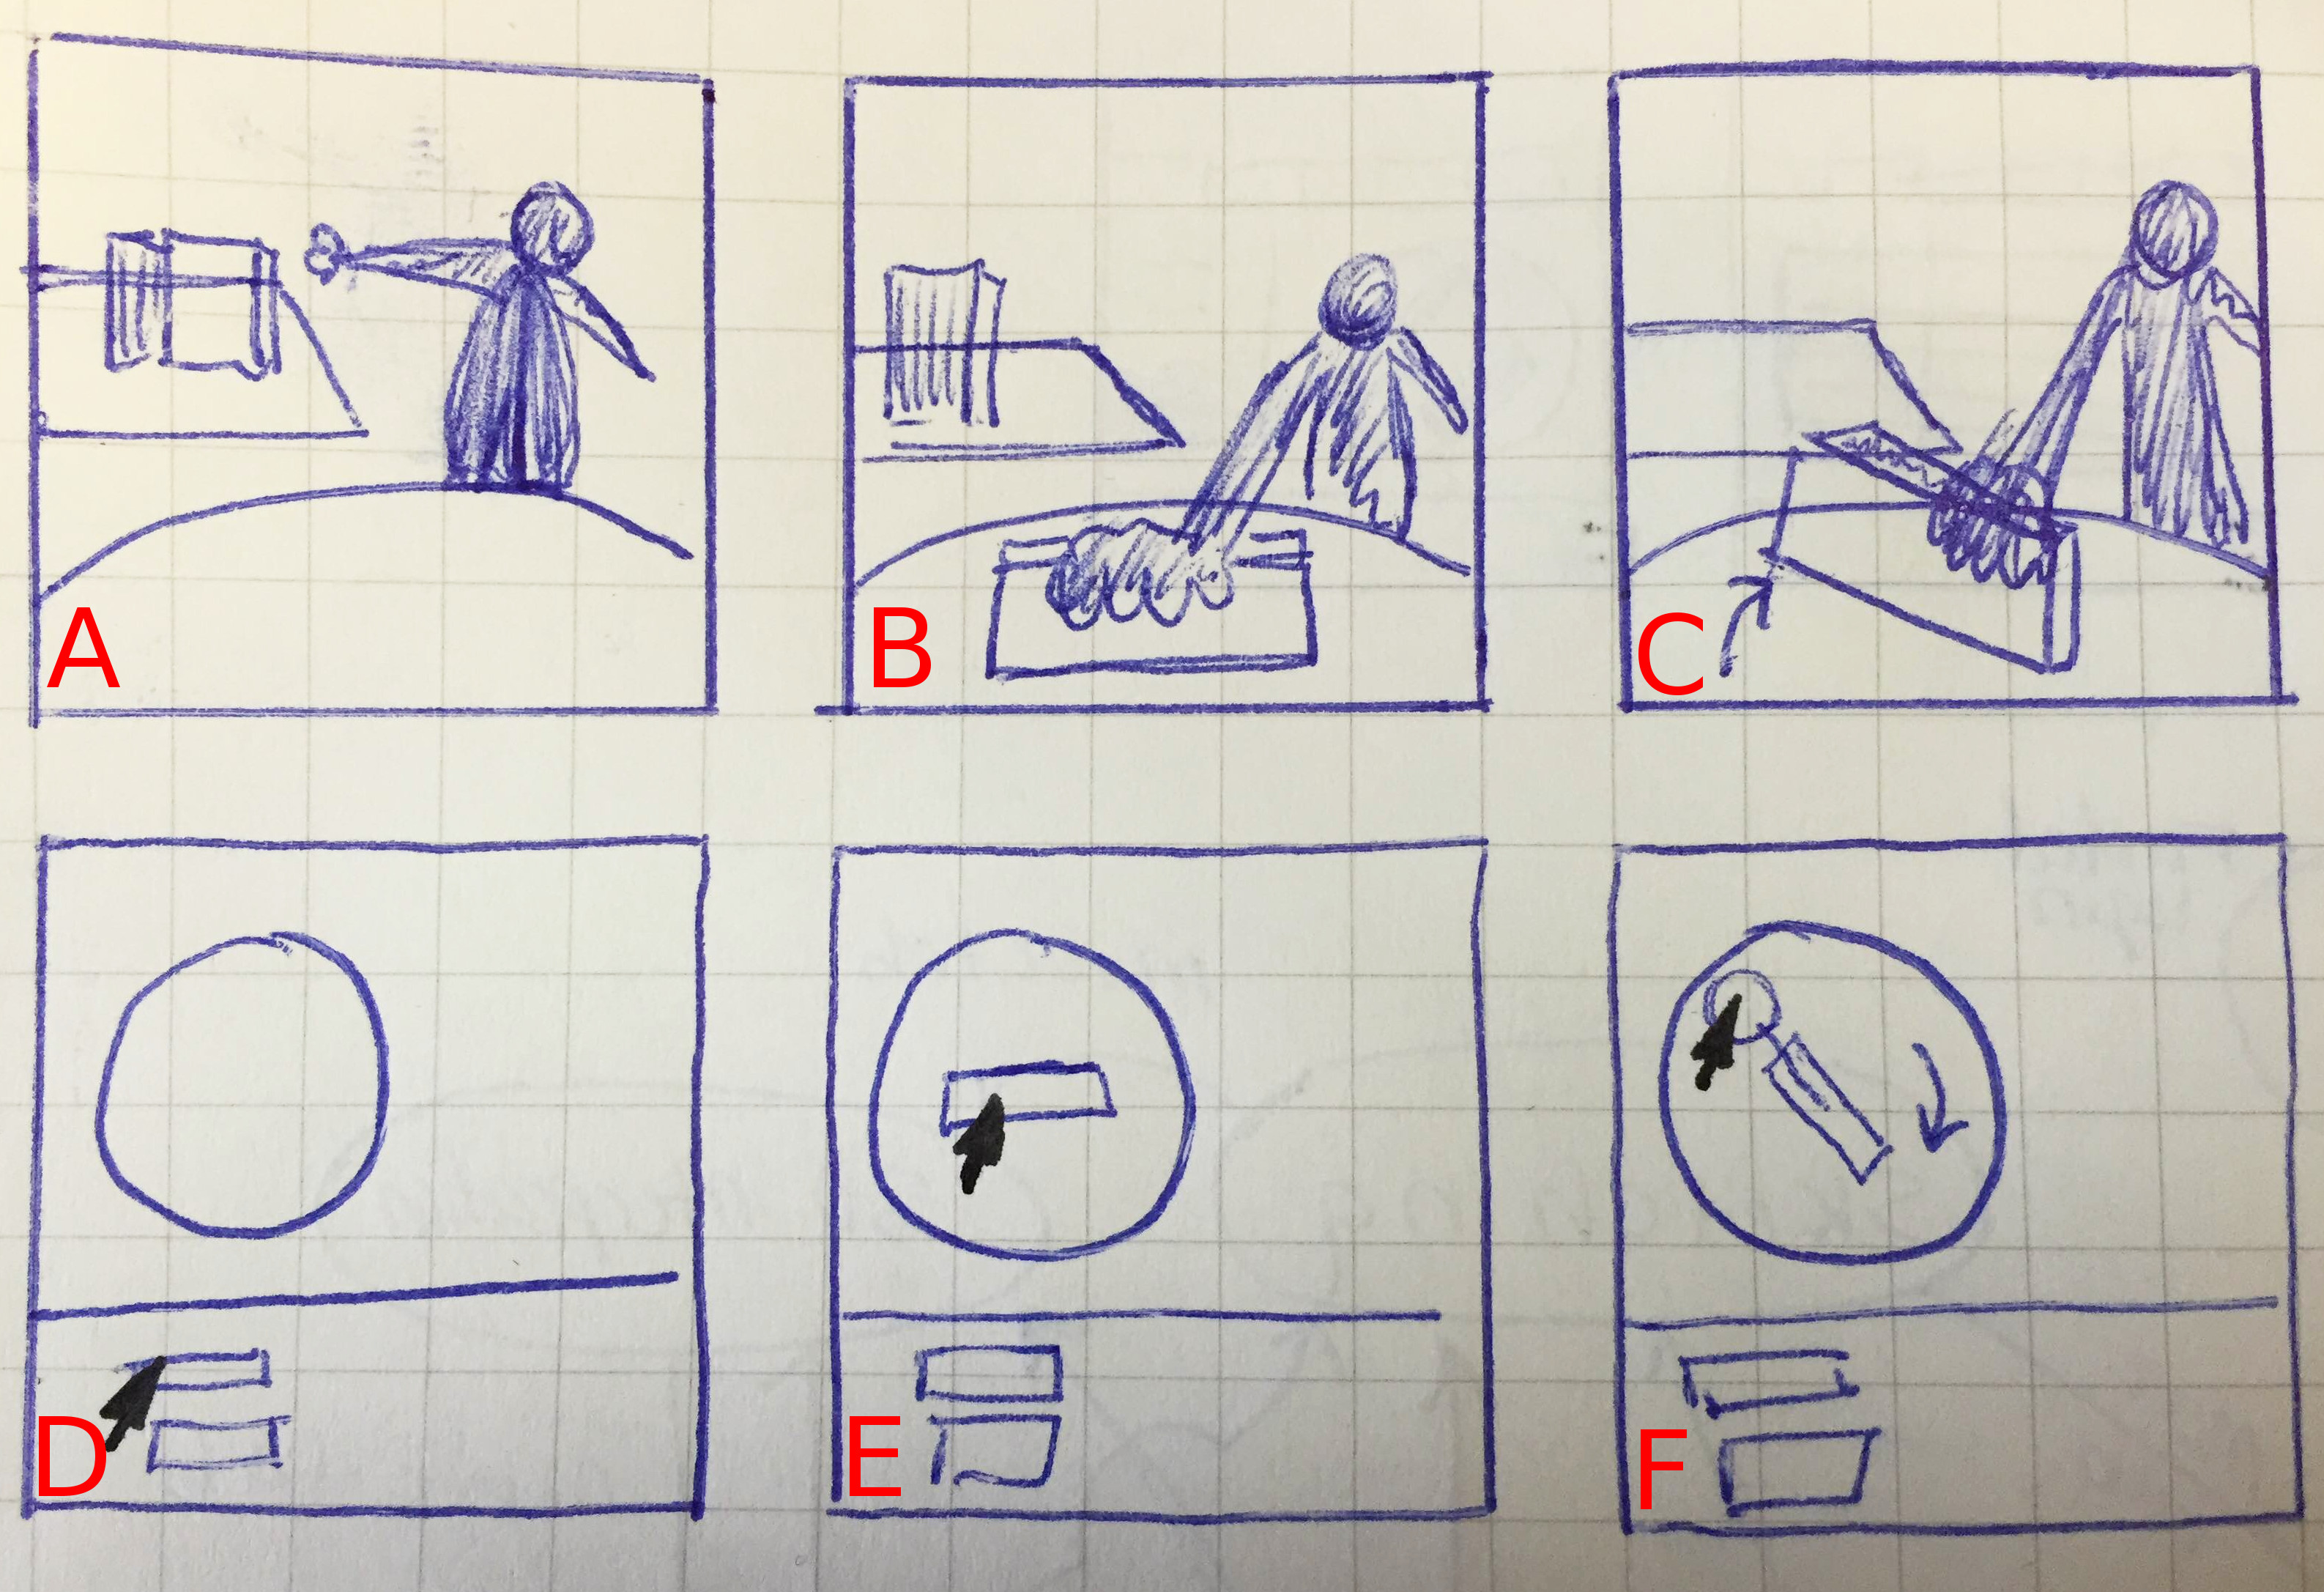
\includegraphics[width=0.8\textwidth]{oldvh}
\end{figure}

\begin{figure}[!ht]
\centering
\caption{How to create walls and windows via the click-draw-release procedure.}
\label{fig:wall_win}
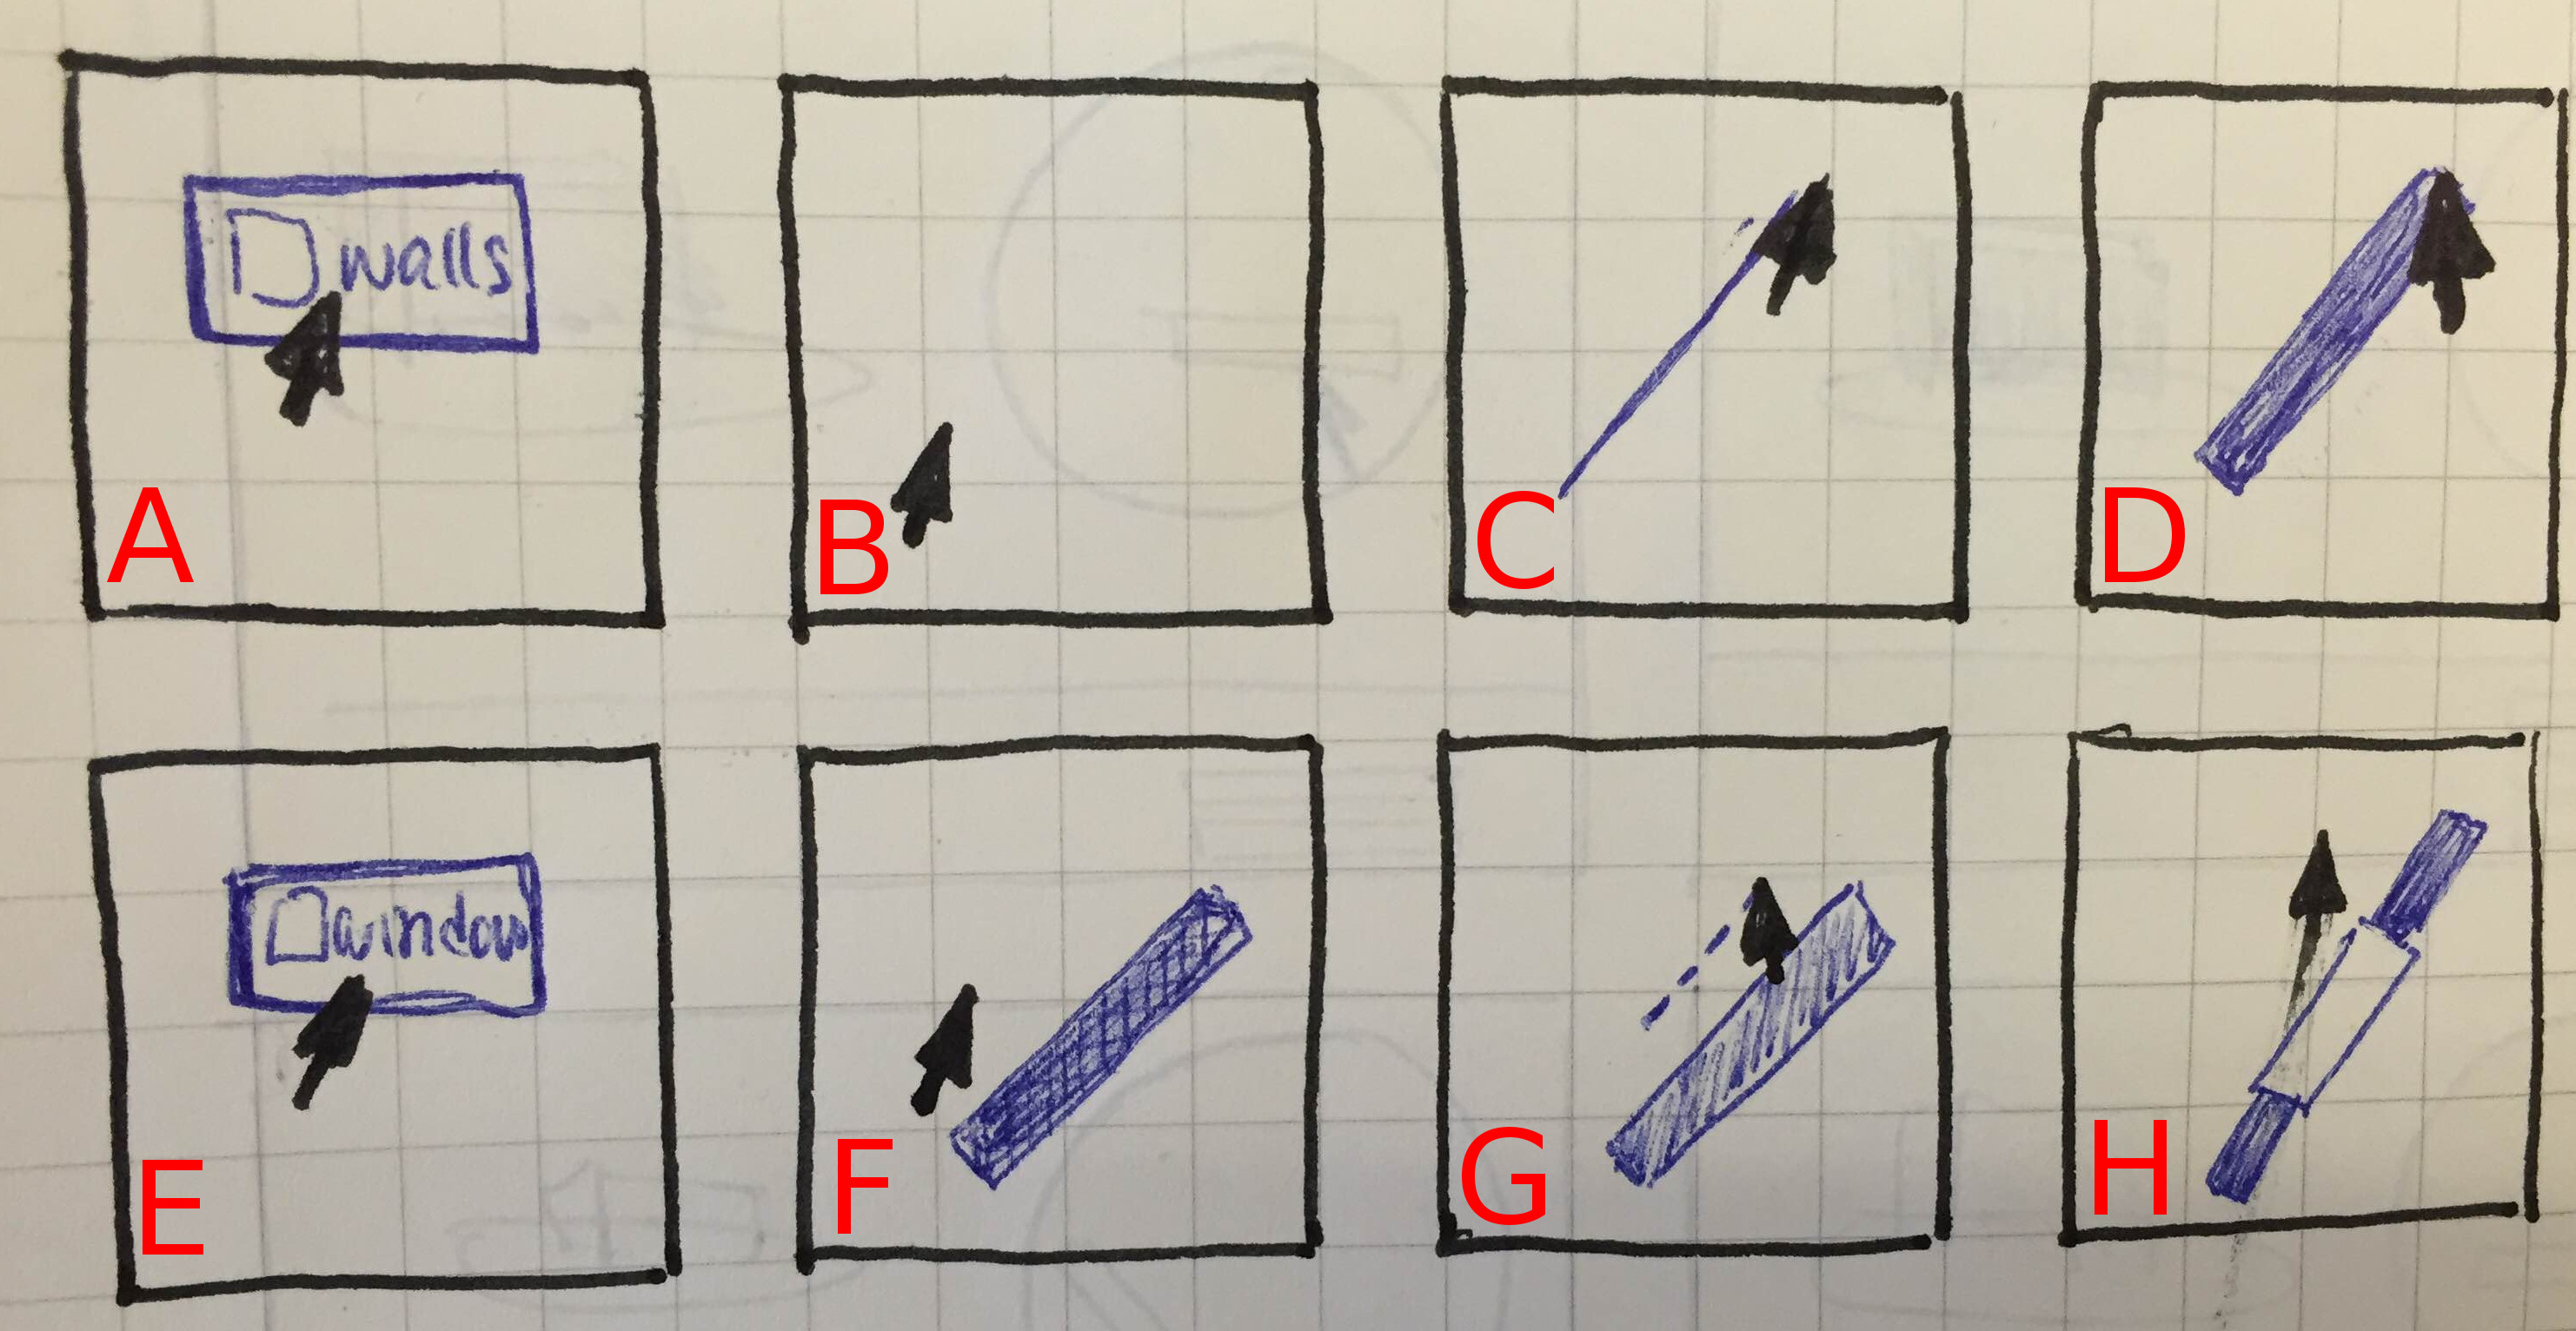
\includegraphics[width=0.8\textwidth]{wall_win}
\end{figure}

% Discussion about Eric's work
Additionally, OASIS is currently undergoing the investigation of a new sketching interface that would allow users to draw free form lines, shapes, and letters.
Using this new sketching interface users could traditionally draw walls and windows to define architectural sketches on OASIS.
User's drawing accuracy can vary dramatically depending on the input devices users are drawing with; common input devices includes computer mouses, touch screens, and pen-based drawing tablets.
This new interface is investigating how to correct users' sketches to  generate the intermediate primitives file required to create  3D closed meshes for simulations.
Extensive A/B testing between these three methods of sketching walls and windows  would be required to to decide which interface is most intuitive to users.

\paragraph{Furniture Placement}

Another difference between OASIS and the Virtual Heliodon is the support of furniture items.
Walls and windows are not the only elements that affect daylighting;
furniture can also occlude, diffuse, and reflect daylight.
Moreover, daylight distribution is scale invariant and as a result the Virtual Heliodon did not concern itself much with communicating to users a sense of scale.
We currently support statically sized furniture items in OASIS, such as beds, desks, and wardrobes.
These furniture items are used to indirectly communicate a sense of scale to users.
Since furniture items cannot be made larger or smaller, users are forced to sketch architectural spaces in respect to the size of furniture items.
Furthermore unlike walls and windows, furniture items are placed into the canvas by first clicking a furniture item button; these buttons are located on the top of the \textit{Sketch a Room} page.
After choosing a furniture item, OASIS will place the item at the center of the canvas.
Furniture items use the same drag-and-drop procedure as mentioned previously in Figure-\ref{fig:oldvh}.
Users can manipulate furniture items via both translations and rotations. 
Furniture items can be rotated along their center axis via FreeTransform handles attached to the furniture item.
Furniture items can also be translated by clicking and dragging on the item itself.
Item manipulation via drag-and-drop procedures are a common UI mechanism. 
Users will be familiar with these mechanisms if they have had experience using either photo editing software or slide-based presentation tools such as Microsoft PowerPoint\cite{todo}.

% Discussion about future work on sketched furniture items + Dynamic scale??
Additionally, OASIS is currently undergoing the investigation of a new sketching interface that would allow users to draw free form lines, shapes, and letters for not only wall and window placement but also furniture placement.
This interface would allow users to freely draw symbols, that represent furniture items, to determine the position and angle a furniture item will be placed into the canvas.
Interpreting symbols is non-trivial and more research is required before A/B testing can be conducted to determine the advantages of freely drawing furniture items.


\paragraph{Removal of Elements}
OASIS also supports the removal of walls, windows, and furniture items.
Since users cannot reposition their drawn walls and windows after their initial placement, the ability to remove and redraw a wall or window is essential.
The removal of all sketch based elements and furniture is done via a click-to-remove process.
To remove items users must first click on the remove button as illustrated in Figure-\ref{fig:remove}A, secondly users must mouse over the item to be removed as shown in Figure-\ref{fig:remove}B.
Items to be removed upon the left mouse button click are highlighted in red as shown in Figure-\ref{fig:remove}C.
No items are removed from the canvas until the user's left mouse button clicks on a selected item.
An alternative removal mechanism would allowed users to drag walls and windows and ``drop'' elements off the canvas. 
This alternative removal mechanism is intended to mimic the Virtual Heliodon's tangible user interface.
While, OASIS does not support this drag-to-remove procedure,  implementing and A/B testing against this procedure would help us understand which removal procedure users find the most intuitive.

% Include figure
\begin{figure}[!ht]
\centering
\caption{How to remove an item from the canvas via the click-to-remove procedure. 
% A) First users must select the remove button located on the ribbon. 
% B) Second the user must move mouse over the time to be deleted. 
% C) Item to be deleted upon left mouse click is highlighted red. 
% D) If the red highlighted item is the correct item to be removed click the left mouse button. 
}
\label{fig:remove}
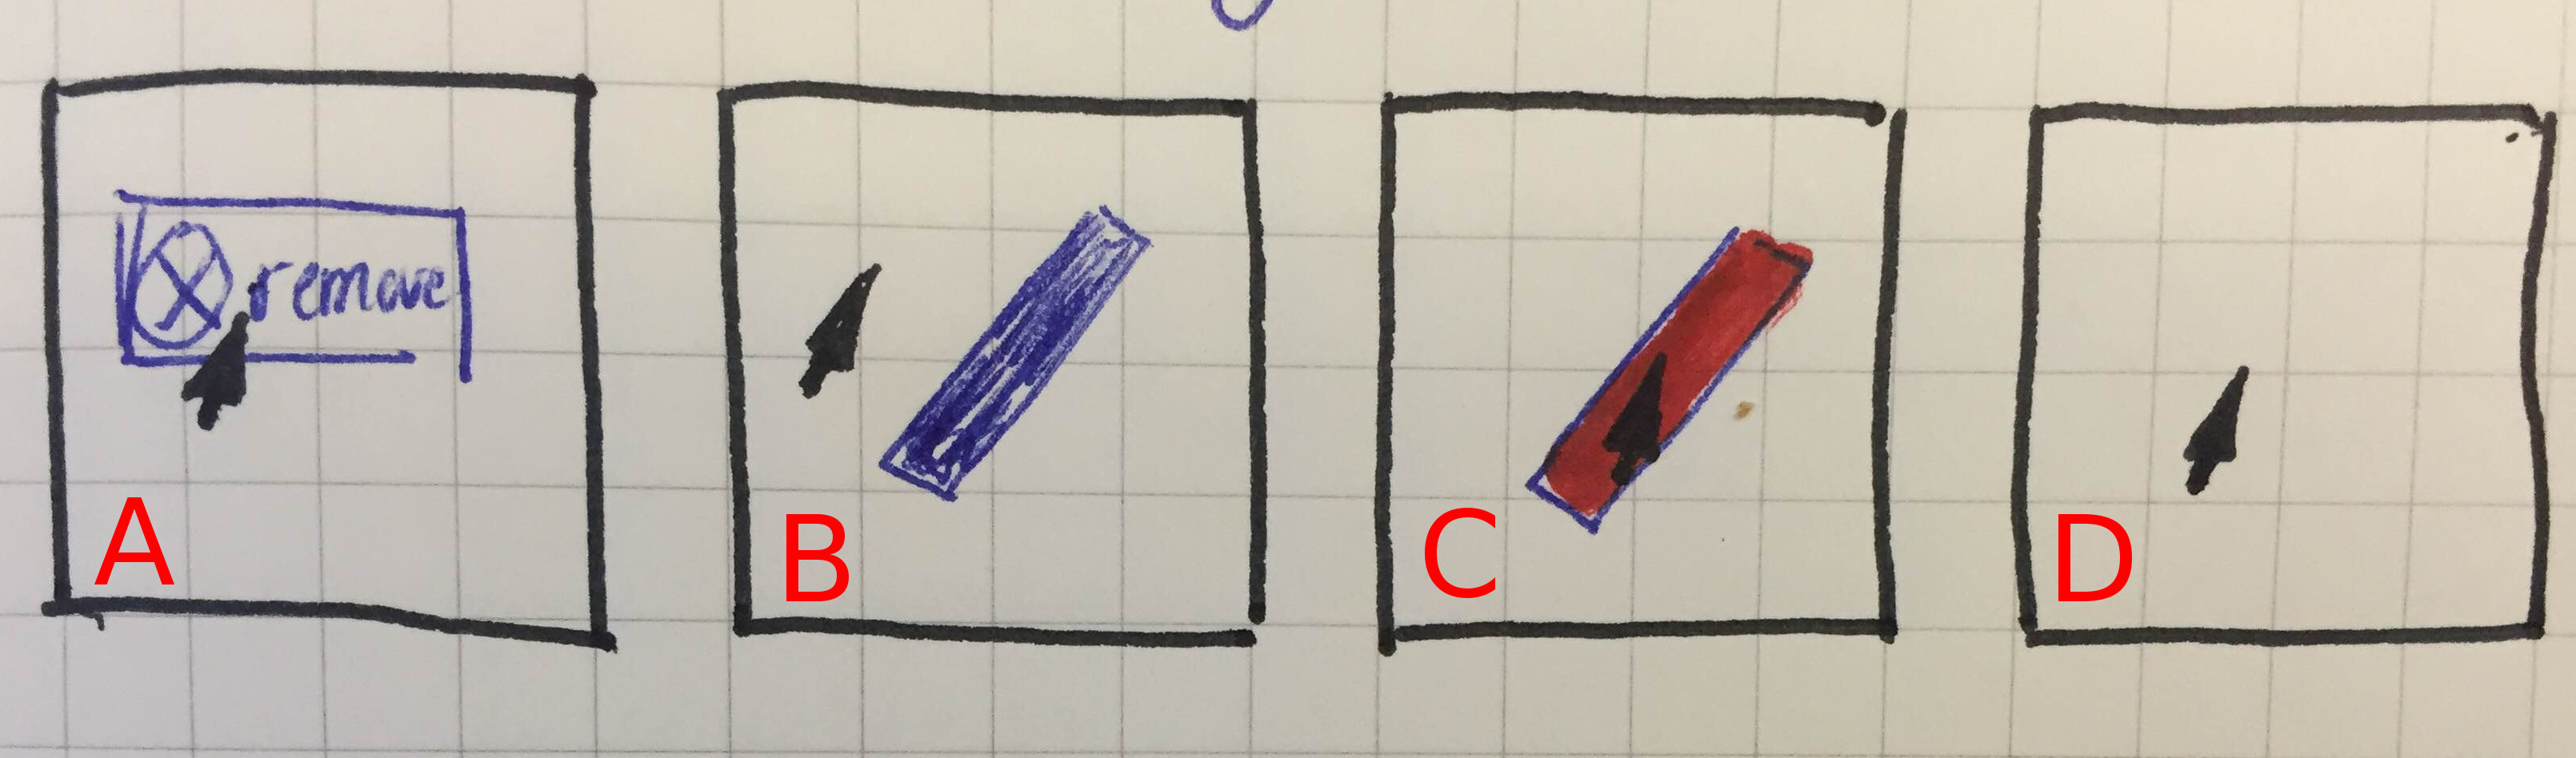
\includegraphics[width=0.8\textwidth]{remove}
\end{figure}

\paragraph{Cardinal Orientation}
% Why is orientation important
The cardinal orientation a of a window has significant impact on daylight distribution in an architectural space.
In OASIS and all daylight analysis tools require that users define cardinal orientation in a architectural space.
Notably, the cardinal orientation of user sketches needs to be defined in order to simulate direct lighting.
% How do we implement it? 
In order to define cardinal orientation users must first click on the orientation button, located in the \textit{Sketch a Room} page's ribbon depicted in Figure-\ref{fig:geoloc}A.
Then users can click and drag anywhere on the canvas to define cardinal orientation.
Specifically, holding the left mouse button on canvas will move the North and South labels around the circumference of the canvas to define the cardinal orientation of the sketch, as shown in Figure-\ref{fig:geoloc}B through D.
% Alternatives
Furthermore, the Virtual Heliodon allows the user to place a north arrow token onto the tabletop to define the cardinal orientation of a physical sketch.
An analogous procedure would require users sketch an arrow on OASIS in order to define the cardinal orientation of their sketches.
Other options include manually typing the model's degree offset from the north arrow; This procedural method of defining the cardinal orientation is common in other daylight software.
Testing would be required to conclude which method of defining cardinal orientation is most intuitive to users.

\begin{figure}[!ht]
\centering
\caption{
How to set the cardinal orientation and geographical location of a sketch.}
\label{fig:geoloc}
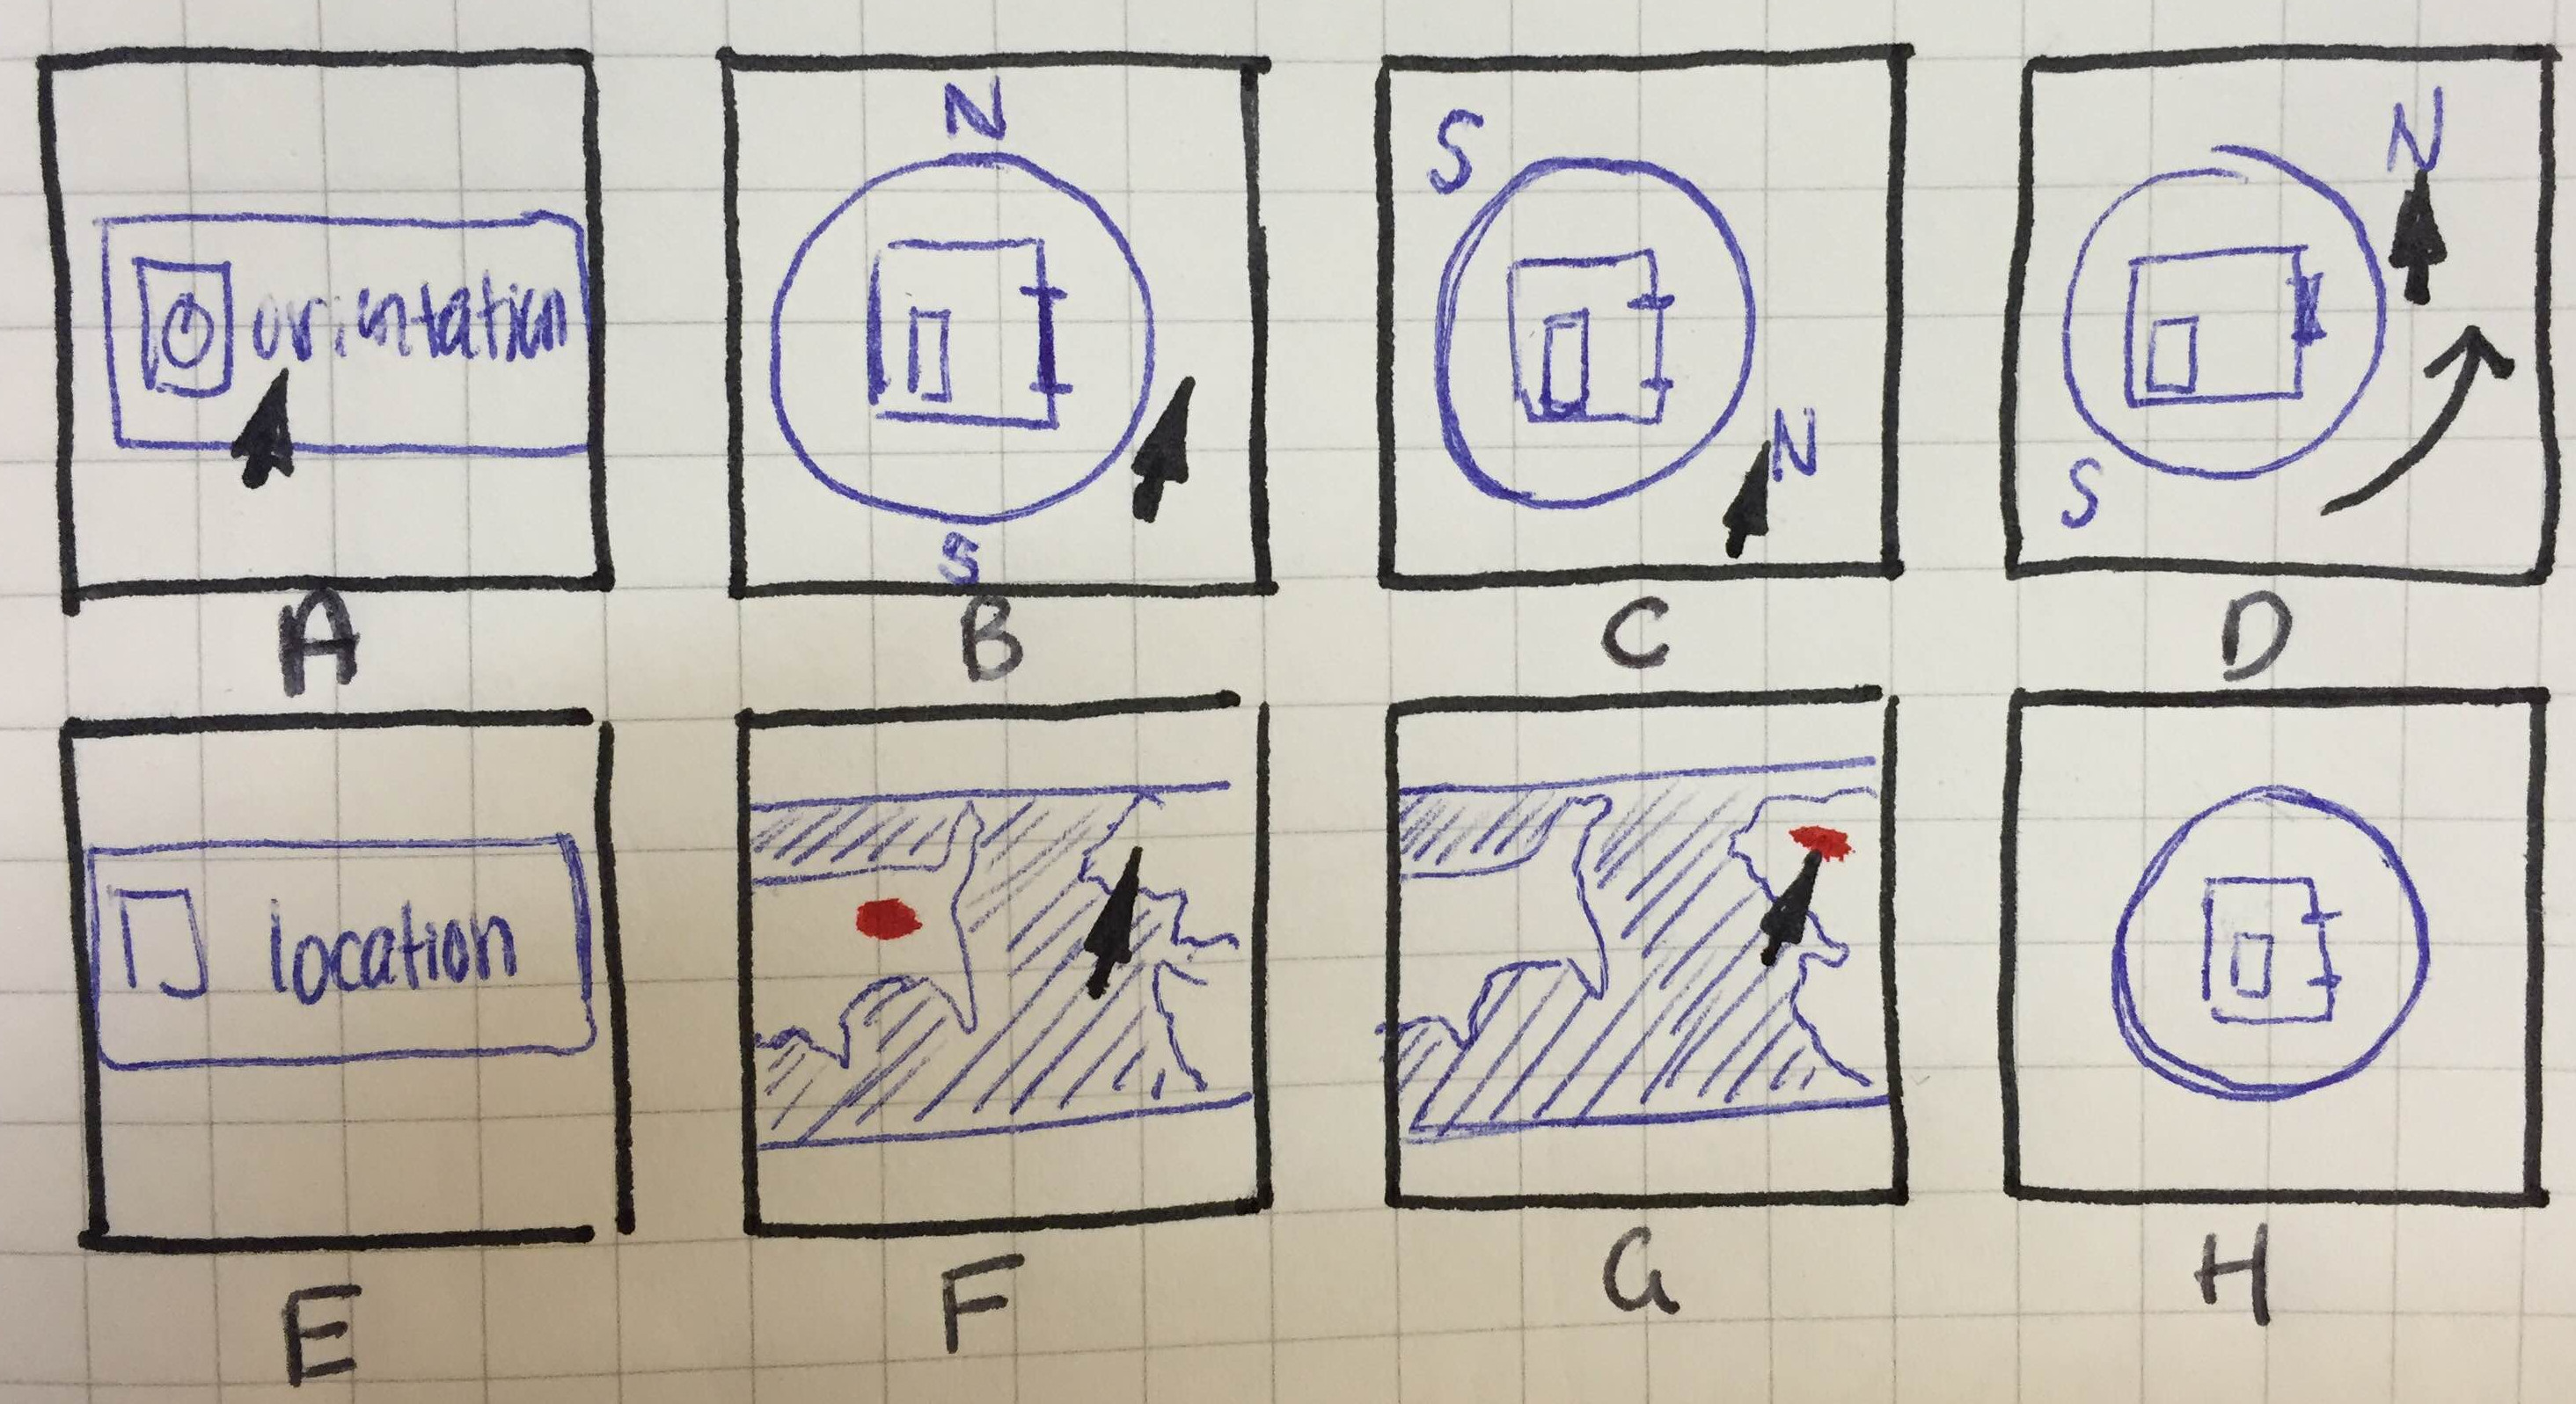
\includegraphics[width=0.8\textwidth]{geoloc}
\end{figure}

\paragraph{Geographical Positioning}
Daylight distribution is  not only dependent on an architectural space's cardinal orientation, but also from its geographic location.
South facing windows in the northern hemisphere experience direct sunlight for most of the day, however north facing windows do not.
In the southern hemisphere, the opposite is true; North facing windows experience direct sunlight and south facing windows do not.
Additionally, the sun's highest point in the sky varies from buildings located in the tropics and buildings located outside them.
For these reasons it is important that in OASIS we provide users a way to define a sketche's geographical location.
To define a geographical location users must click on the location button next to the orientation button depicted in Figure-\ref{fig:geoloc}E.
Clicking the location button will bring up a map projection where users can select their model's geographical location by clicking anywhere on the map, as shown in Figure-\ref{fig:geoloc}F and G.
Once the user has selected a location, a red marker is placed on that location and the map  disappears revealing the sketching interface, as depicted in Figure-\ref{fig:geoloc}H.
Users do not need the exact latitude and longitude values because we intend OASIS to be an early design tool. 
Furthermore, daylighting varies significantly depending on what hemisphere a model is located. Daylighting also varies depending on a model's location relative to the equator.
Inaccurately selecting a geographical position off by an entire state or even country will not vary daylighting results much.
Figure-\ref{fig:geoloc} illustrates how a sketch's cardinal orientation and geographical location are defined.
The Virtual Heliodon offers no analogous interface to define geographic location of sketches. 
All sketches in the Virtual Heliodon are set to Troy, NY.
Most daylight analysis software allows users choice from a variety of major cities to define a model's geographic location;
others allow users the ability to input exact geographic coordinates.
Again, testing would be required before any conclusions can be drawn about which method is most intuitive to users for defining the geographic location of models.

\section{3D model viewer}

\paragraph{Sketch Interpretation Viewer}\label{3dviewer}
The sketch interpretation viewer is located on the \textit{Generate 3D Model Page}. This is a simple viewer that displays the 3D watertight mesh created from users' architectural sketches. Users can zoom, rotate, and pan on this viewer. Additionally, walls facing the viewer are rendered transparently so that users can view the inside of their sketch from any view point, as seen in Figure-\ref{viewer}A.
It is important to display this information to users because, although the physical sketch interpretation algorithm generally matches users' intentions, there are cases where the 3D watertight mesh does not match users' intentions. Allowing  users to view the interpretation of their model, before continuing to analyzing an unintentional architectural space, will save users time. Additionally it would provide users a chance to make alterations,  so that the physical sketch interpretation algorithm better understands users intention; this can be accomplished by better defining an architectural space or simplifying complex models to lesser levels of detail.
Alternative interfaces have been considered, however not pursued at this time. An alternative interface would actively invoke the physical sketch interpretation algorithm upon any updates to a sketch. An up to date interpretation of their sketch would be visible to users as they actively sketch out their model. Live interpretations would let the user know exactly when a generated model deviates from the user's original intention; Knowing exactly when the interpretation between the user and our algorithm deviates would allow the user to make alterations to their sketch without having to guess as to which elements in the sketch contributed to the misinterpretation. The development of such an interface is left as future work.

\begin{figure}[!ht]
\centering
\caption{On the left is an example of the sketch interpretation viewer and on the right is an example of the daylight rendering viewer.}
\label{fig:viewer}
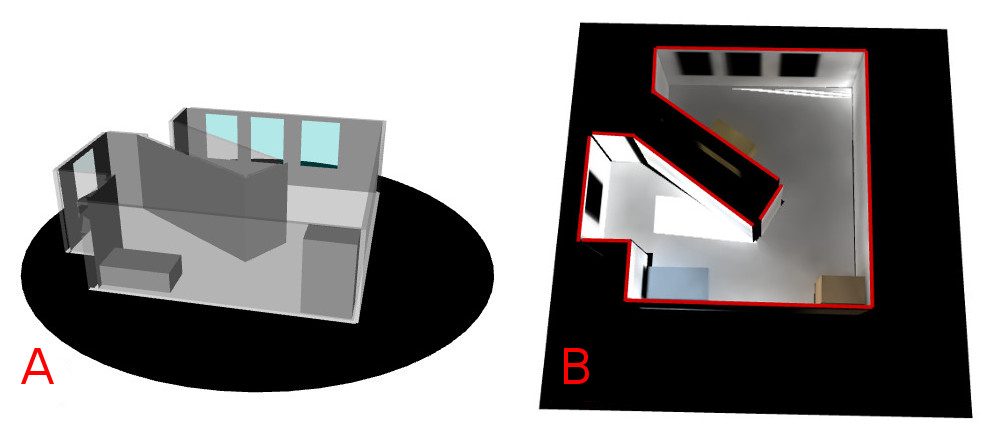
\includegraphics[width=0.8\textwidth]{viewer}
\end{figure}

\paragraph{Daylight Rendering Viewer}
The daylight rendering viewer is located on the \textit{Analyze Simulation} page. 
This viewer supports the same navigation controls as the sketch interpretation viewer. However, there are two visualization modes users can choose from on the daylight rendering viewer; this viewer supports daylight renderings and false color visualizations. These two visualization modes are illustrated in Figure-\ref{false_color}.
In Figure-\ref{false_color}B the false color visualization brings users attention to areas that suffer from over and under illumination. This feature was ported from the Virtual Heliodon and displays a textured checkerboard image on surfaces that fall below or above specific thresholds in relation to the daylight rendering engine's illumination values\cite{nasman2013evaluation}. Red checkerboard patterns are used to represent over illumination and blue checkerboard patterns for under illumination.Our intention as an early design tool is to have users analyze the daylight visualization results on the \textit{Analyze Simulation} page. From their analysis users are either satisfied with the distribution of daylight in their model or choose to make renovations. Improvements include making alterations to diffuse lighting if over illumination is a problem. Additionally, improvements could include making windows larger or changing the orientation of the room to make better use of daylight. Overall, the daylight rendering viewer should not be the final step on users' work flow in OASIS, but instead be a point of evaluation that communicates to users where problems lie so that they may go back and make edits to their design and continue the cycle of the creative iterative design process. 


\begin{figure}[!ht]
\centering
\caption[The two visualization modes of the daylight rendering viewer.]{The two visualization modes of the daylight rendering viewer. On the left is a daylight rendering of a model and on the right is a false-color visualization of a model highlighting areas that suffer from over and under illumination.}
\label{fig:false_color}
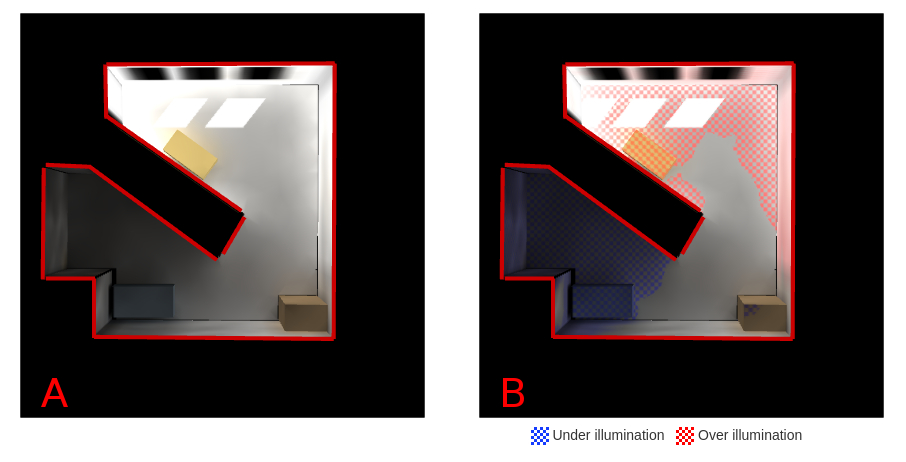
\includegraphics[width=0.8\textwidth]{false_color}
\end{figure}

\paragraph{Share A Model Viewer}
Current work is being done on a \textit{Share A Model} viewer. This viewer would allow users to share models via generated URLS.The purpose of this viewer is two fold. Firstly, I suspect it would make sharing models between users much easier than sharing accounts or taking screenshots of OASIS and replicating sketches via tracing. In essence this feature would allow users to fork models from other users. Secondly, I hope this feature would allow users to share models between non-users, including family and friends. Rather than taking screenshots, non-users can visit the URL provided from a user and view the 3D rendering of a model without needing to sign up for an account. Figure-\ref{fig:share} illustrates the viewer in its current state. As mentioned, this stand alone viewer is currently under development.
\begin{figure}[!ht]
\centering
\caption[Share A Model viewer in its current state of development.]{Share A Model viewer in its current state of development. No user registration is required to view a model.}
\label{fig:share}
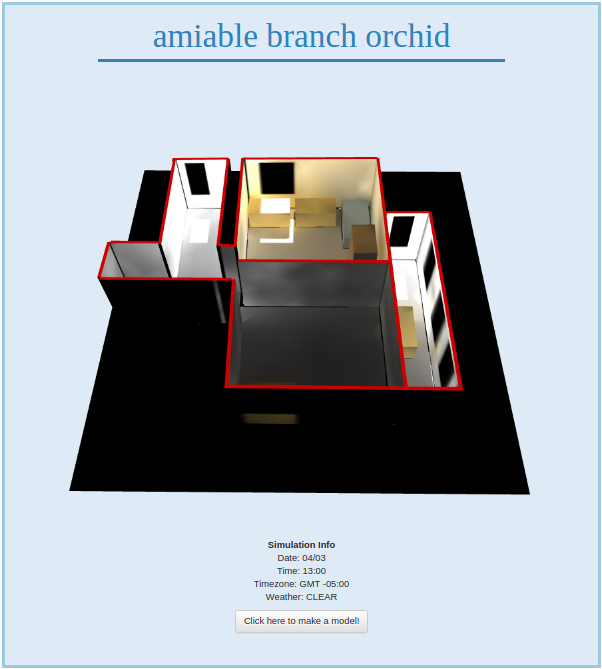
\includegraphics[width=0.8\textwidth]{share}
\end{figure}

\section{General Web Application Design}

\paragraph{Ribbon Design Choice} As mentioned previously in section-\ref{ui_importance} the user interface of any tool is of great significance. 
For that reason I choose to use a ribbon interface to organize the pages and tools on OASIS. 
The Ribbon interface is common to contemporary Microsoft products and even a few other daylight analysis tools\cite{todo}.
The hope is that organizing tools and pages in an interface that might be familiar to users would make using OASIS easier. Figure-\ref{fig:ribbon} illustrates the similarities between our interface and Microsoft Word.
Additionally, I made the design choice of having OASIS appear in its own web browser window after being launched. Being in a standalone window is meant to further communicate that OASIS is a stand alone application.


\begin{figure}[!ht]
\centering
\caption{On the top is Microsoft Word's ribbon and on the bottom is OASIS' version of a ribbon.}
\label{fig:ribbon}
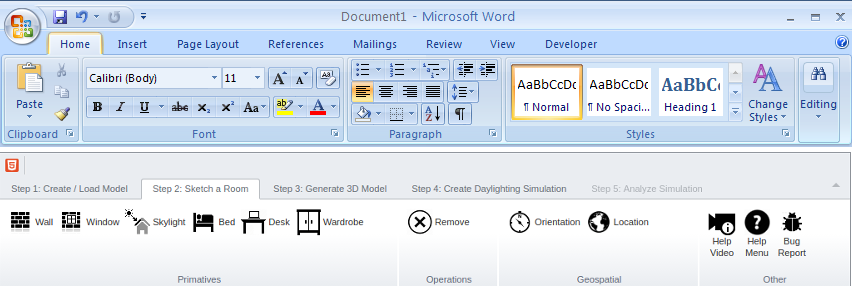
\includegraphics[width=1\textwidth]{ribbon}
\end{figure}

\paragraph{Nonlinear Navigation in OASIS}
Although we recommend beginners navigate pages on OASIS linearly, nonlinear navigation is also supported. For example, non-first time users can log into OASIS and jump directly to the \textit{Generate a 3D Model} page. This page will display the last model the user was working on before leaving OASIS. Similarly, a non-first time user logging back into OASIS can jump to the \textit{Sketch A Room} page and the last sketch the user was working on before leaving OASIS will be displayed. 
Users can nonlinearly move between the \textit{Create/Load Model} page ,  the {Sketch A Room} page , the \textit{Generate a 3D Model} page and the \textit{Create A Daylight Simulation} page without state changes to OASIS. However, the \textit{Analyze Simulation} page is only reachable through the viewing of a daylight simulation from the \textit{Create A Daylight Simulation} page. Additionally, when viewing the daylight renderings of a model on the \textit{Analyze Simulation} page a state change occurs. Viewing a rendering has the same effect as loading a sketch; this change will be reflected if a user navigates to the \textit{Generate a 3D Model} page or the \textit{Sketch A Room} page. Overall, OASIS supports nonlinear navigation to save advance users time from having to follow pages linearly.
%Figure-\ref{fig:states} illustrates the navigation between pages on OASIS
% \begin{figure}[!ht]
% \centering
% 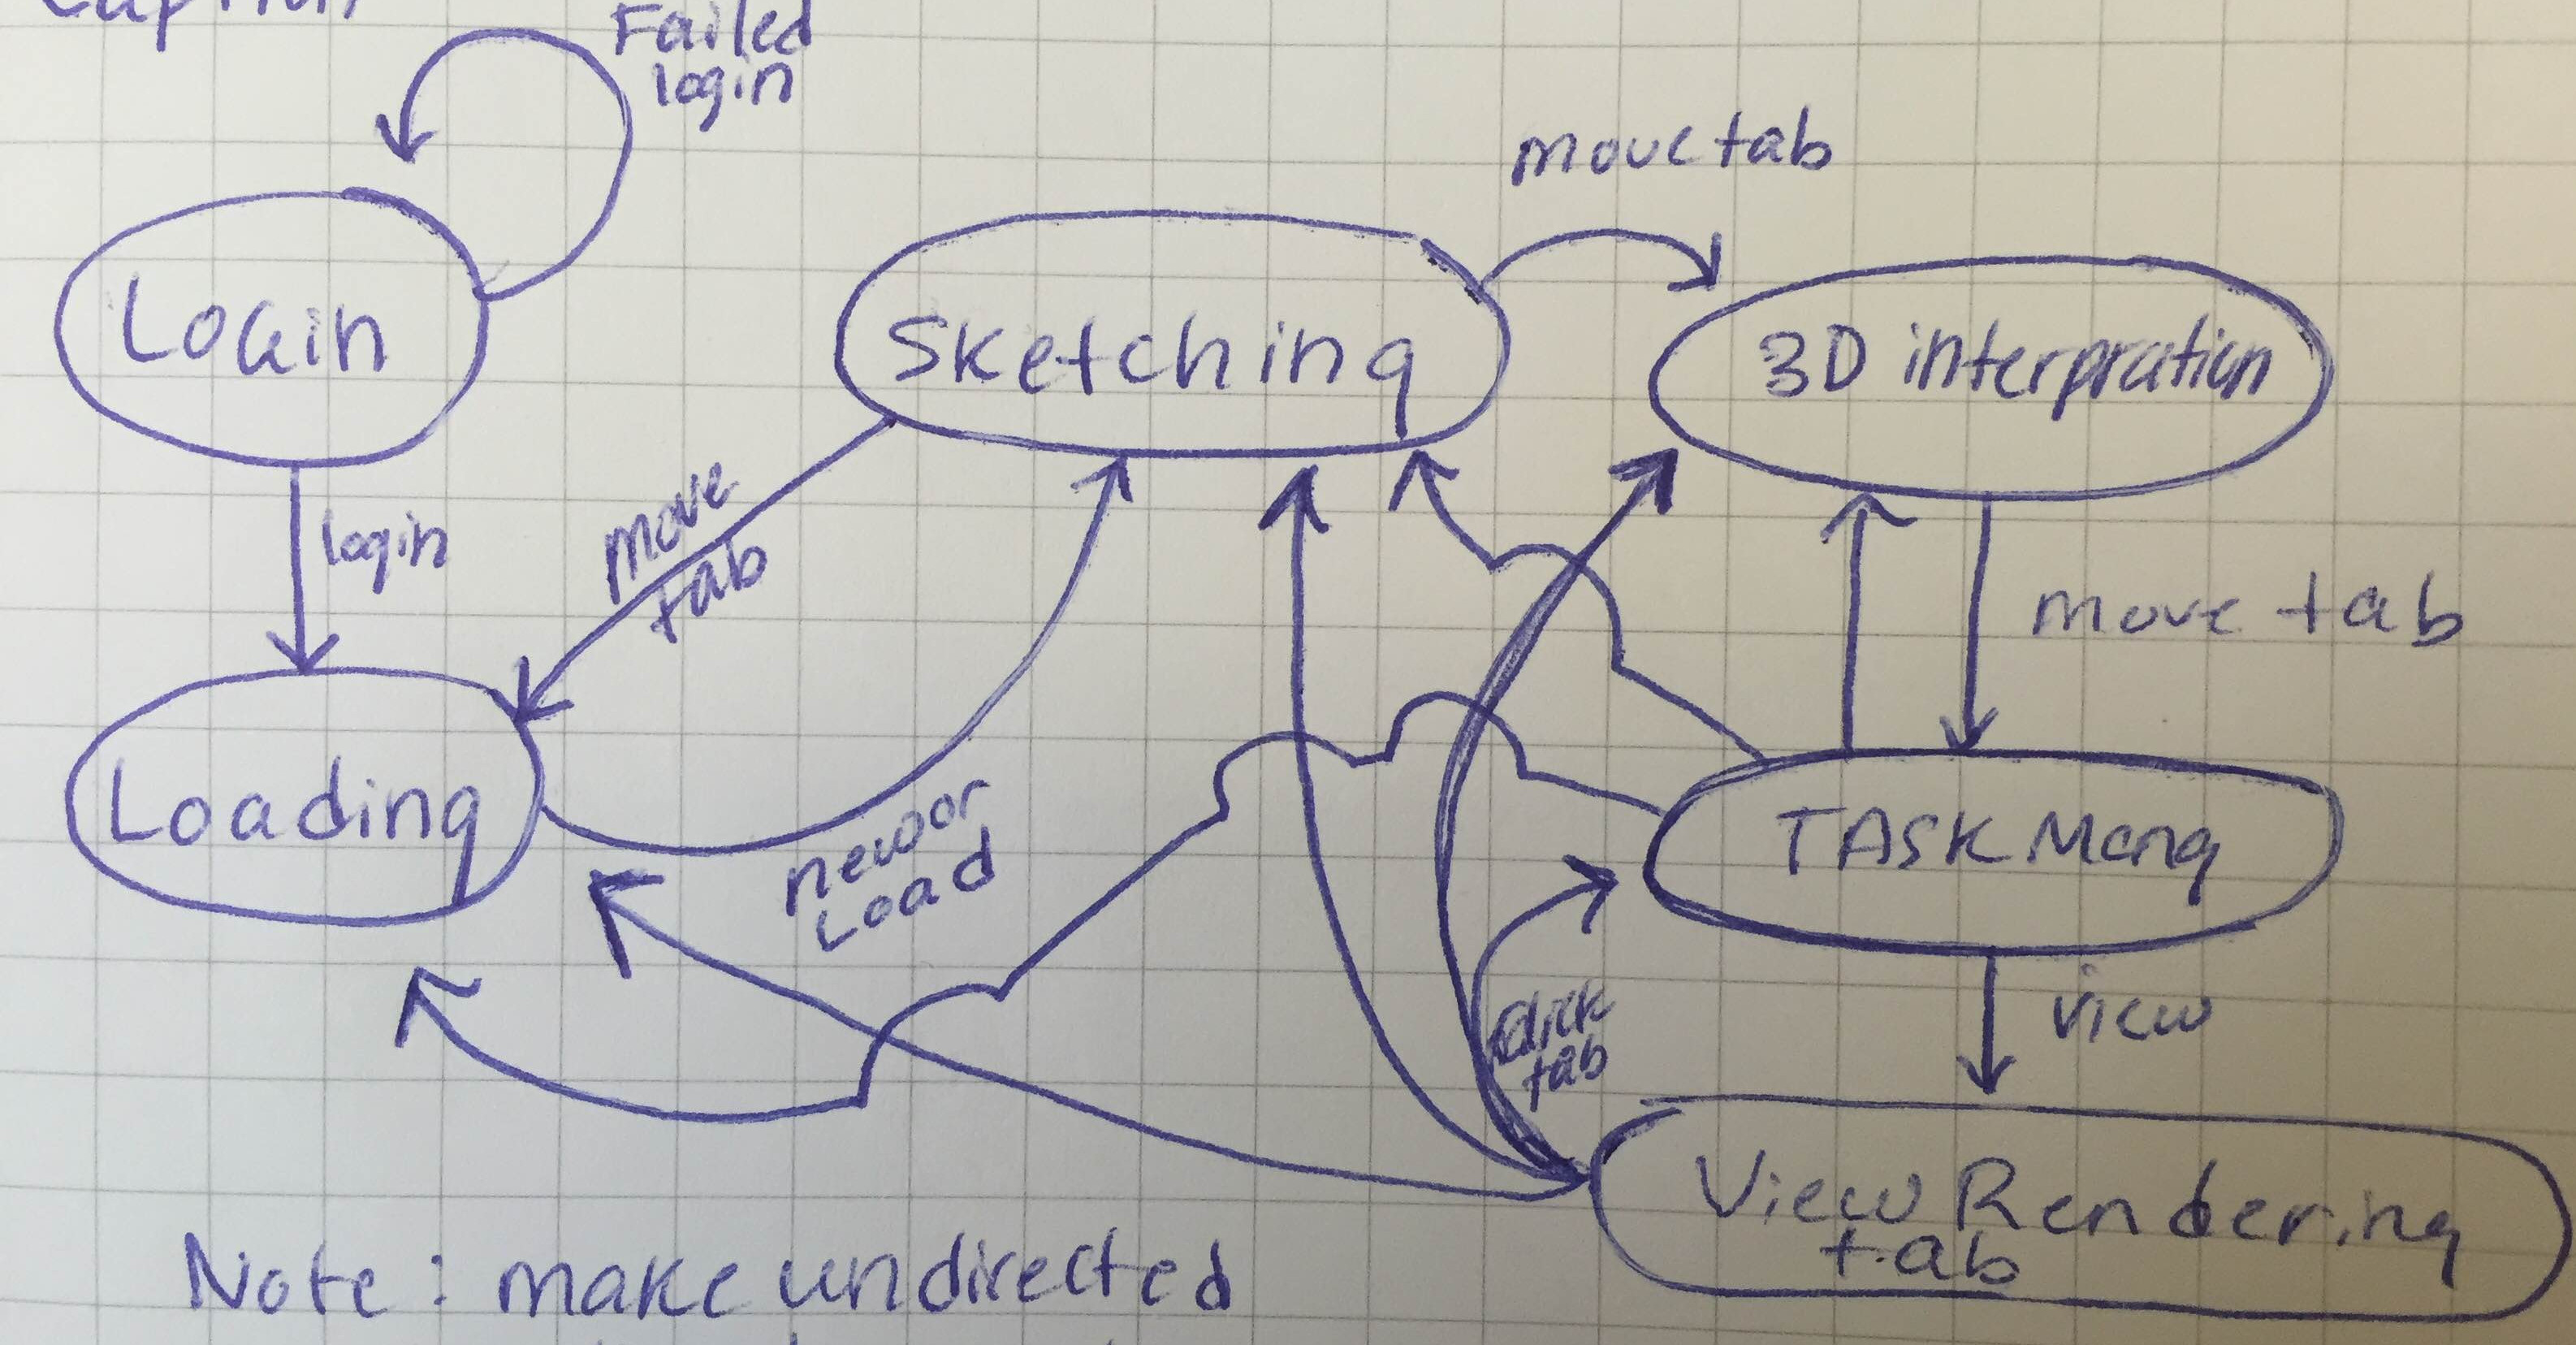
\includegraphics[width=0.8\textwidth]{states}
% \caption{This is a navigation diagram between pages and menus on OASIS.}
% \label{fig:states}
% \end{figure}


\section{Problems Encountered During System Design}

\paragraph{Computational Intensive Procedures}
One of the first problems encountered in the design of OASIS was the fact that both the physical sketch interpretation algorithm and daylight rendering engine are computationally expensive. Furthermore, the daylight rendering engine requires specialized graphical processing hardware. Porting both of these components to work on multiple platforms would have been time intensive and hard to maintain. As a result we provide a server-client architecture for the generation of 3D models and daylight visualizations. Users define a set of parameters per rendering request and then submit a request to the server. The server is aware of all pending requests and handles all requests in a first come first serve manner. The model and the input parameters are then passed along to the daylight rendering engine. We then map the output  textures onto the walls, furniture items, and floor in the 3D model displayed on OASIS. Another important usability feature added was the caching of previous renderings on the machine hosting OASIS. The caching of previous renderings allows users to quickly view previous renderings without having to rerun the simulations on the server.	
 
\paragraph{Storing Models}
% Saving on Database
Another problem I faced during the design of OASIS was ensuring the safety of user created content. 
A simple solution to the problem would have been saving all user created content directly on the server hosting OASIS.
However, this carries the risk of being corrupted during development. Additionally, if the server hosting OASIS were to suffer technical difficulties then user created content could potentially be lost.Our solution to the problem was storing user data both on the server hosting our web application and a database maintained by an outside party.
Most user data can be recreated given an intermediate primitives file and rendering arguments. Data that cannot be recreated such as the intermediate primitives files and rendering arguments are stored in the outside database.
User data that is reproducible using the physical sketch interpretation algorithm and daylight rendering engine is stored on the server hosting OASIS. This separation of non-reproducible and reproducible user data is done for safety. Keeping non-reproducible data off the server hosting OASIS would allow us to recreate all user created data if necessary from data stored on the outside database.
% future mentions of load balancing

\paragraph{Training Users}
Another issue I faced during the design of OASIS was anticipating how much help users would require when using OASIS for the first time. At first we offered a ten minute tutorial video of how to generate a model, perform renovations, and generate daylight renderings. An unofficial small user study of under ten people was conducted to test if making this video available was helpful in training users. Most users skipped the video and did not understand how to use OASIS. As a result we then created help menus on all pages of OASIS. To access the help menu users would have to click the \textit{Help Menu} button located on the top right of OASIS. Again, we ran a small user study of under ten people to test if users would understand how to use OASIS given a help menu.
Results from that unofficial study showed that users did not use the help menu.
Lastly, a short 1 minute long help video was created that walks users through generating daylighting renderings of a single model. This video automatically plays when users first log into OASIS.
A formal pilot study was conducted that asked users if they found OASIS was easy-to-use and results from that pilot study are analyzed in Chapter 5. Overall, it seems that the problem of training users was solved by recognizing first time users and offering them a short tutorial video that did not cover all the features in OASIS, but just the essential features required to start.

\section{Implementation Details}
There were many frameworks used in the development of OASIS.
A few notable ones include RibbonJS, RaphaelJS, and WebGL.
RibbonJS is a JavaScript port of Microsoft's ribbon user interface.
RibbonJS not only supports the generation of a ribbon but also provides event handlers.
Another framework used in our sketching interface is RaphaelJS\cite{todo}.
RaphaelJS is a 2D vector graphics library for JavaScript. 
I use RaphaelJS to create the 2D graphics for walls, windows, and furniture items.
 I also use the FreeTransform extension for RaphaelJS\cite{todo}. 
The FreeTransform extension is used to create FreeTransform handles so that users may easily rotate and reposition furniture items.
Lastly, I use WebGL to display renderings and 3D interpreted models on OASIS. 
Specifically, I use the WebGL library ThreeJS\cite{todo}.
ThreeJS is a framework that provides useful wrappers for common WebGL functions.
WebGL is supported on most web browsers including Google Chrome and Mozilla Firefox\cite{todo}.
Displaying complex 3D models on web browsers is non-trivial.
As a result WebGL gives us the unique ability to have our sketching interface online in a platform independent manner.


\section{Chapter Summary}
% Summary of what we covered
All things considered, OASIS is an alternative interface for key components in the Virtual Heliodon. Although both OASIS and the Virtual Heliodon share similar objectives, the two systems provide different interfaces for the design of architectural spaces. Specifically, OASIS focuses on its autonomy and availability to a broad range of users. 
Research has shown that user interfaces can make or break an application and as a result OASIS aims to provide an intuitive interface for both experts and novices. Careful thought was put into the design of the sketching interface currently used on OASIS; however, alternative methods to sketching operations are being considered for future A/B testing. \\

Additionally it is important to display the interpretation of users' online sketches. OASIS usually understands the user's intentions in an online sketch, however there are cases where the generated 3D model does not match the user's original intentions.
Allowing  users to view the interpretation of their model, before continuing to analyzing an unintentional architectural space, will save users time.
Similarly, the daylight rendering viewer is important because it gives users information about the daylight distribution in created architectural spaces. 
This information, coupled with false-color visualizations, allows users to evaluate daylighting. All in all, both design choices taken in creating the  sketching interface and viewers on OASIS were made to provide users an intuitive  interface for the generation of architectural models and running of simulations. Other general design choices such as  using ribbons for organizing pages on OASIS and support of nonlinear navigation between pages on OASIS were made to benefit both expert and novice users. \\

Furthermore, there were several problems encountered in the design of OASIS.
OASIS is a solution to the non-trivial problem of providing a tool available to all users that relies heavily on computationally expensive processes. The client-server architecture was used to allow users to create physical sketch interpretations and render daylight visualizations at interactive rates without the need of specialized computer hardware. 
Additionally, OASIS keeps users' created content safe by storing non-reproducible content separate from the server OASIS is hosted on. In the event that the machine hosting OASIS fails, no user created content will be lost.
We will be able to recreate all reproducible user content from the saved non-reproducible content stored on the external database.
It is also important to note that OASIS was not developed from scratch but rather from multiple existing tools and frameworks including the Virtual Heliodon, RibbonJS, RaphaelJS, and WebGL.
The Virtual Heliodon was used for its physical sketch interpretation algorithm and daylight rendering engine.
RibbonJS was used for its  emulated ribbon interface.
RaphaelJS was used for its 2D vector graphics.
And lastly,  WebGL was used for the ability to display 3D meshes on users' web browsers.

    \chapter{Pilot User Study} \label{sec:userstudy}
Aside from creating an online architectural interface for simulations, I also made preparations for a pilot user study aimed at answering a few evaluation questions about the usability of our online interface.
I hypothesize that if OASIS is publicized to users online, then anonymous online users will construct models in our sketching interface and create daylight renderings for analysis.
Additionally, this pilot user study will serve as a test for OASIS.
In theory there should be no issues when multiple users are logged into OASIS;
However, OASIS has yet to be used by multiple users simultaneously.
To summarize, I anticipate  that this pilot user study will provide us valuable feedback to improve OASIS.
\\

\section{Previous User Studies}
	% Point I'm trying to get across is that OASIS will make collecting models easy. Just make the point.	
	The physical sketch interpretation algorithm has gone through three previous user studies.
	The physical sketch interpretation algorithm has gone through three previous user studies.
	While these previous studies gathered over 300 physical sketches, they did so from a medium sized pool of users.
	This pool of users varied from 13 to 30 participants across all previous user studies.
	It is also important to note that these studies each took, on average, 2 months to complete data collection and were comprised of mostly students at Rensselaer Polytechnic Institute.
	The cost of effort to collect a model is relativity high compared to OASIS.
	Overall I speculate that the number of models produced on OASIS will be quantitatively larger  and from a broader range of users than previous user studies.

\section{Availability of OASIS}
% OASIS can be used by anyone who is interested
In order to provide an architectural sketching interface for both novices and experts,  we must support as many platforms as possible. While experts my go to great lengths to install a piece of software, novices might not expend as much effort or have the technical skills required to install software.
As a result of being a web application OASIS is platform independent, has no installation process, and can globally apply updates to all clients.
Additionally, having a web application lends itself naturally to using a client-server architecture.
In OASIS I leverage the server to both service our web page and run computationally expensive processes on behalf of clients.
Namely, these computationally expensive processes are the physical sketch interpretation algorithm and the daylight rendering engine.
Both of these processes are computed on a specialized lab machine rather then locally on users' machines.
My hope is that leveraging the server to run computationally expensive components in OASIS will prevent potential participants from opting out of our pilot user study due to hardware limitations and will provide a homogeneous user experience across all platforms.


\section{User Feedback  Collection in OASIS}
	% This section should be strictly about what we collect, not how we collect it.
	In OASIS I collect two types of data from users. Both active and passive data are collected from users while they use our tool. Active data refers to the feedback, models, and comments users actively provide. The relationship between users, models, renovations, and renderings can be seen in Figure-\ref{fig:rel}. Passive data refers to data not actively provided by users, such as the length of time a user spends on a page, the average wait time before rendering request are handled, and other information about users usage of our application. We collect both types of data to get a clearer idea of how users perceive OASIS and how users interact with our tool. Active feedback data collected is associated with either a specific user, model, renovation, or rendering in OASIS. This includes questions pertaining to users' past experience and education in fields such as architecture and the visual arts. Additionally, we are interested in users experience with other 3D modeling or simulation tools for architecture. We also ask users questions pertaining to their sketches. For example, we ask users to categorize their sketches; daylighting practices vary for bedrooms, offices, classrooms, and more. Understanding what kind of space a user is sketching is important for future analysis.	Aside from asking users to categorize their sketches, we also ask users to elaborate on how confident they are in their accuracy of their sketches.  While, I might not be interested in users' confidence in recreating sketches in this pilot user study, future studies can compare users' created sketches to real blue prints to gain insight into how users perceive and sketch architectural spaces from memory.

	We are also interested in collecting feedback on model renovations. Particularly, we are interested in if the 3D models generated by the physical sketch interpretation algorithm matches users' original intentions. As stated previously, the physical sketch interpretation algorithm usually matches users' intentions, however there are cases where  3D models generated is not representative of users' original intentions. Users can make modifications to models, defined as renovations, for a variety of reasons. They could be trying to alter the distribution of daylight in their architectural space or trying to better communicate their intentions to the physical sketch interpretation algorithm. Lastly, we ask users questions about renderings they created. Some questions generally ask about the effectiveness of OASIS as a daylight analysis tool; Other questions are more specific such as if a user understands the results of a particular rendering. All questions presented to users can be viewed in Chapter-\ref{sec:appendix}.

				
	As mentioned before we also collect passive data.
	Specifically, we collect how long users spend on each page of our interface and how long users wait for both  sketch interpretations and daylight renderings.

	\begin{figure}[h]
	\caption[The relationship between users, models, renovations, and renderings.]{The relationship between users, models, renovations, and renderings. Users are associated with a set of models, models are associated with a set of renovations, and renovations are associated with a set of renderings.}
	\label{fig:rel}	
	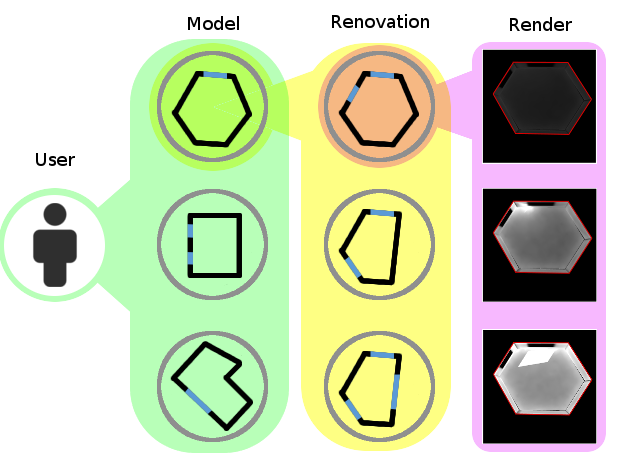
\includegraphics[width=0.8\textwidth]{relationship}

	\end{figure}


\section{Data Collection}
	In order to collect feedback on OASIS we have to first host the application online, and then bring potential users' attention to the application. As an online study, we must invite users to participate in order to collect feedback.
	Personally inviting individuals to use our tool might be cumbersome and slow going, so we hope inviting users in large groups by advertising in social media networks and on online bulletin boards will result in increased user participation. One advantage of using online bulletin boards is that they are organized by users' interest.  We use this organization to target users who might have an interest in daylighting or architecture. For this study we focused on advertising on  Reddit\footnote{https://www.reddit.com/[Accessed: Apr 8 2016]}. Reddit is a popular online bulletin board where users organize themselves by interest into smaller bulletin boards known as subreddits. In these subreddits users can share content such as links, images, and text that is relevant to the subreddits's interest. Table-\ref{fig:reddit} list a few relevant subreddits and their respective user sizes that we plan to advertise OASIS to.
	

	\begin{table}[ht!]
	\centering
	    \caption{Subreddits and their respective subscribers sizes.}
	    \label{fig:reddit}
	    \begin{tabular}{ | l | l | }
	        \hline
		    Subreddit               & Subscribers  \\ \hline
		    InteriorDesign 			& 78,750        \\ \hline
		    RPI 			        & 3,939         \\ \hline
		    Floorplan    			& 1,175         \\ \hline
		    UserExperienceDesign    & 1,128         \\ \hline
		    GreenArchitecture 		& 607          \\ \hline
		    YoungArchitects 		& 236          \\ \hline
	    \end{tabular}
	\end{table}

	Additionally, in this pilot study we target users who are likely to create models of Rensselaer Polytechnic Institute dormitories. If a user communicates that they are sketching an RPI dormitory by answering feedback questions, we ask the user to elaborate on which RPI dormitory they are sketching. We are collecting this data for future studies where we can analyze users' sketches of RPI dormitories against blue prints of those dormitories. Doing so would give us insight into how accurately users can sketch their dormitories. To begin, we plan on advertising OASIS on a subreddit unofficially affiliated with RPI. Moreover, we plan on also advertising our tool on campus. As done in previous studies we wish to leverage the Rensselaer Polytechnic Institute School of Architecture in order to collect feedback from users with formal education in architecture. Students with formal education in architecture are likely to have experience with architectural design software and daylighting. Their feedback, as non-novices, I believe will be useful because their previous experience with related software can help us improve OASIS.


\section{Chapter Summary}


	In addition to the creation of OASIS, I also conducted a pilot user study. 
	I hypothesize that if OASIS is publicized to users online, then anonymous online users will construct models in our sketching interface and create daylight renderings for analysis.
	Also, I speculate that the number of models anonymous online users will construct on OASIS will be quantitatively larger and from a broader range of users than previous user studies conducted on the Virtual Heliodon.
	Collecting both active and passive feedback from users will help us better understand where improvements to OASIS can be made and how users currently experience OASIS.
	Lastly, in order to collect as much feedback as possible we plan on advertising OASIS on social media outlets, online bulletin boards, and on campus.
	To summarize, I anticipate  that this pilot user study will provide us valuable feedback to improve OASIS.






    \chapter{Pilot User Study Results And Analysis} \label{sec:results}

	%intro paragraph
	%intro paragraph
	%intro paragraph
	%intro paragraph
	%intro paragraph


\section{Participants Background Feedback}

In the two week timespan that OASIS was publicly available 57 users registered and participated in our pilot user study.
I recruited participants for our pilot user study from social media outlets and online bulletin boards; specifically, we advertised OASIS on Facebook\cite{todo} and subreddits\cite{todo} that share relevant interest to daylighting and architecture. Also note that at the  current time of this study, OASIS was yet to be advertised to students at Rensselaer Polytechnic Institute. Moreover, both Facebook and Reddit have a wide range of users with varying experiences.

Figure-\ref{fig:rpi_affilation} shows the affiliation of participants who registered on OASIS.
As shown in Figure-\ref{fig:rpi_affilation} a majority of participants that provided their affiliation are not affiliated with RPI. 
This is a big change from previous user studies, where all the participants were RPI affiliated.
Additionally, Figure-\ref{fig:rpi_affilation} shows that the majority of participants that are affiliated with RPI, are undergraduates.
It is also interesting that the majority of participants did not provide information on their affiliation with RPI.
This could be either because they did not notice the feedback questions on OASIS, or chose not to answer these questions.
Checking if users answered other feedback questions might provide insight as to whether users did not notice this question or purposefully skipped it. 
Specifically, 65\% of participants did not provide feedback on their affiliation, and not all participants who claimed to be affiliated with RPI specified how they were affiliated;
About 2\% of participants have unknown affiliations with RPI.
The difference between RPI affiliated participants and non-RPI affiliated participants could be a direct result of when we recruited participants for the pilot user study.
During the pilot user study we advertised towards non-RPI affiliated users and did not yet advertise to RPI affiliated users. 

	\begin{figure}[!ht]
	\centering
	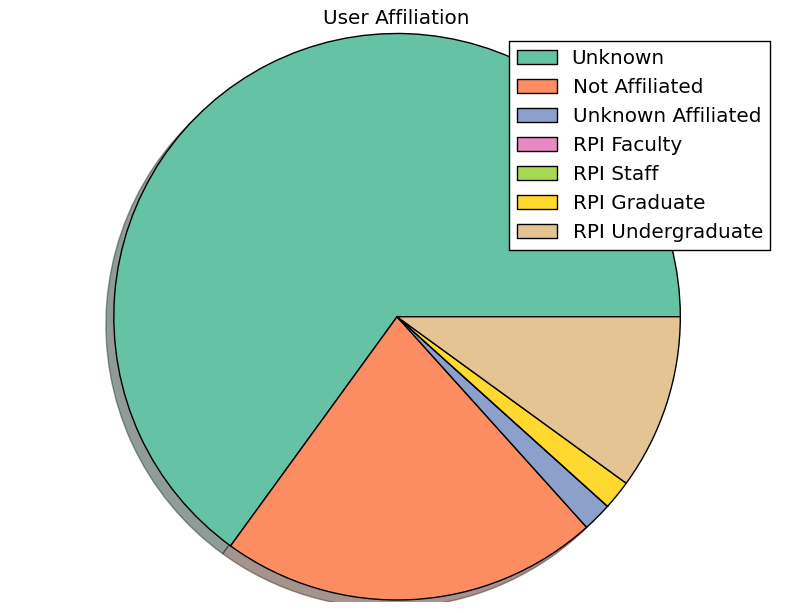
\includegraphics[width=0.8\textwidth]{rpi_affilation}
	\caption{User affiliations of participants on OASIS}
	\label{fig:rpi_affilation}
	\end{figure}

	\begin{figure}[!ht]
	\centering
	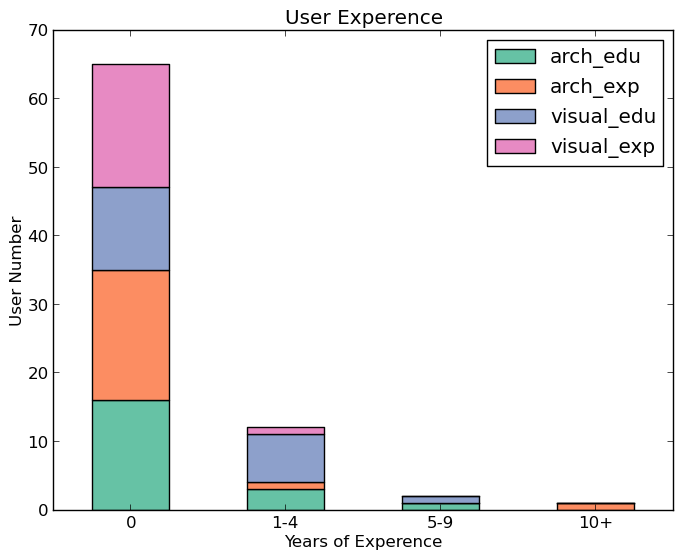
\includegraphics[width=0.8\textwidth]{exp_edu}
	\caption{Architecture and visual arts experience of OASIS participants }
	\label{fig:exp_edu}
	\end{figure}

Similarly, I asked our participants about their experience with architecture and visual arts.
Figure-\ref{fig:exp_edu} shows the distribution of participants' formal education and job experience in both fields of architecture and the visual arts.
A majority of our participants expressed that they have no experience with any of the related fields;
As a result, these participants will be referred to as non-experts or novices.
Also a majority of those participants that have experience, generally have only 1-4 years of exposure to formal architecture education or formal visual arts education.
However, there is one user registered on OASIS that claims to have over 10 years of job experience in architecture.
Aside from asking about architecture and visual arts experience, I also let participants elaborate on other relevant experiences. 
Some of our participants have had experience in civil engineering, electrical engineering, studio arts, user experience design, and architectural engineering with a focus in lighting.
While our current set of participants does not have much experience with architecture, they do encompass a broad range of related fields.\\

\begin{figure}[!ht]
	\centering
	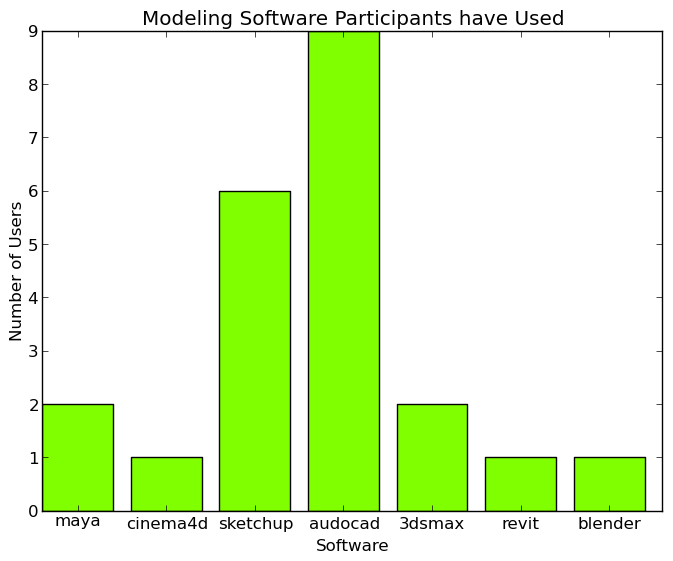
\includegraphics[width=0.8\textwidth]{software_exp}
	\caption{Participants' experience with 3D Modeling Softwares}
	\label{fig:software_exp}
\end{figure}

Furthermore, I also asked participants to provide a list of 3D modeling software they have had exposure to.
As seen in Figure-\ref{fig:software_exp} participants have had the most experience with AudoCad\cite{todo} and SketchUp\cite{todo}. 
A few participants have had experience with 3dsMax\cite{todo} and Maya\cite{todo}.
Again, we let participants elaborate on their experience with other 3D modeling software. 
Other 3D modeling software, not shown in Figure-\ref{fig:software_exp}, that participants have had experience using include SolidWorks\cite{todo}, AGI32\cite{todo}, Dialux\cite{todo}, and Daysim\cite{todo}.
Note that AGI32, Dialux, and Daysim are not specifically 3D modeling tools but rather used for daylight analysis and performance.
From user feedback collected in our pilot user study on participants' affiliations, experience in related fields, and exposure to modeling software, shows that OASIS was used by a wide variety of users.

\begin{figure}[!ht]
	\centering
	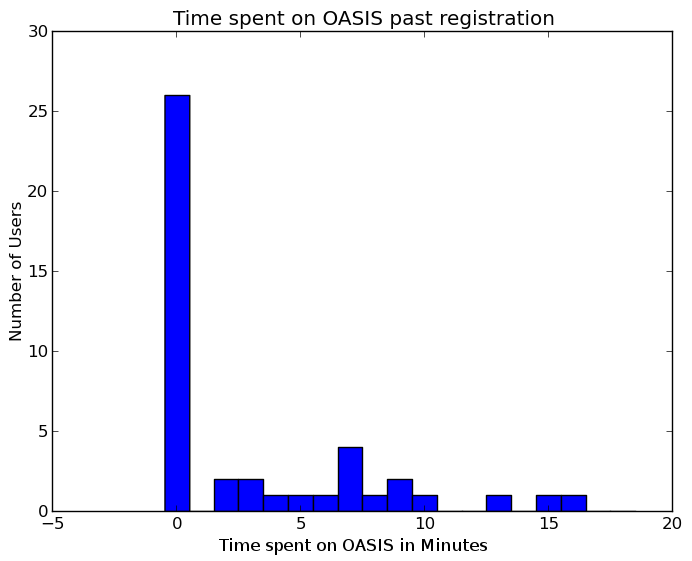
\includegraphics[width=0.8\textwidth]{time_oasis_hist}
	\caption{Distribution of time spent on OASIS per user}
	\label{fig:time_oasis_hist}
\end{figure}

In addition to observing if OASIS was used by a broad range of users, I also wanted user feedback on the usability of OASIS.
Analyzing data on how participants spend their time  on OASIS can provide insight on user behavior.
Figure-\ref{fig:time_oasis_hist} illustrates the distribution of participants in relation to their time spent on OASIS.
Note that OASIS keeps track of the amount of time users spend on each page by timing when a user visits and leaves a page. We make the assumption that users who stay on the page for longer than an hour are non-active and time they spend on that page is not valid.
From Figure-\ref{fig:time_oasis_hist} it is clear that the majority of users registered and participating in the pilot user study spent no time on the actual interface.
On the other hand, the average time spent per participant is about 12 minutes, excluding participants that do not spend longer than a minute on OASIS past registration.
Although our user retention rate is low, I suspect that the voluntary nature, anonymity, and absence of renumeration in our pilot user study plays a significant role in the large number of participants who register and do not use OASIS.
Also  the large number of participants who register and do not use OASIS  could be a direct result of not having a tutorial for most of the pilot user study.
Users who are confused as to what to do on OASIS might have just left before creating a model.

\begin{figure}[!ht]
	\centering
	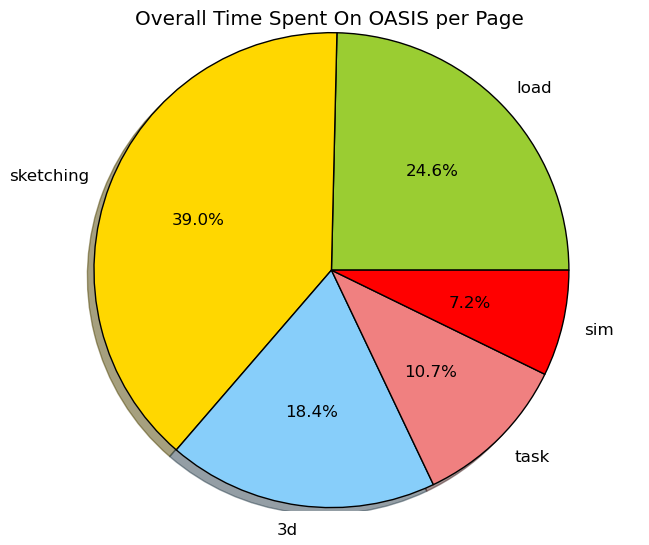
\includegraphics[width=0.8\textwidth]{time_chart}
	\caption{Breakdown of time spent on OASIS pages}
	\label{fig:time_chart}
\end{figure}

Figure-\ref{fig:time_chart} illustrates participants' time spent on OASIS per page.
Moreover, Figure-\ref{fig:time_chart} shows that participants spend 36\% of their time on the \textit{ Sketch a Room} page.
Next participants spend 23\% of their time on the \textit{Create/Load Model} page.
It is important to note that first-time users have the option of viewing a short tutorial video; 
the 1 minute long tutorial video coupled with redirection to the \textit{Create/Load Model} page after logging in, could directly contribute to the large portion of time participants spend on the \textit{Create/Load model} page.
Surprisingly, the page participants spend the least amount of time is on the \textit{Analyze Simulation} page. 
On the \textit{Analyze Simulation} page users can view daylight renderings of user designed models.
On average participants spent only 8\% of their time analyzing their designed models;
when compared to the 25\% of time participants spend on viewing 3D interpretations on the \textit{Generate 3D model} page, the time spend on the \textit{Analyze Simulation} page seems remarkably low.
We expect users spend a majority of their time on creating sketches and analyzing daylight simulation results.
Stressing the importance of daylight analysis in an updated tutorial video might help guide users to the \textit{Analyze Simulation} page.
The difference between time spend on these two pages could stem from the fact that the \textit{Analyze Simulation} page is the final page new users visit when navigating OASIS linearly.
Furthermore, all of the temporal data collected on pages in OASIS could be effected by time spent writing feedback questions, multi-tasking while leaving OASIS running in the background, and leaving OASIS before visiting all pages.
 
\section{Usability Feedback}

Most of the feedback collected on the usability of OASIS is qualitative.
Quantitative boolean feedback would not fully capture how participants are experiencing our sketching interface;
As a result, I collect qualitative feedback to gain insight into how users perceive OASIS.
Table-\ref{fig:fun} list feedback collected from 14 participants concerning what participants found fun or interesting in our sketching environment.
Overall, 6 of the participants mentioned that the interface was either fun or easy-to-use.
However, some participants found window placement non-intuitive; 
other participants had difficulty with the limited primitives we provide.
While, we did not explicitly ask for what users found difficult in this specific feedback question, their response will be taken into consideration.
The participant who found window placement difficult states that they tried to ``leave a gap between walls to define where to place windows''.
I suspect that the participant, with this issue, must have not seen the tutorial video or not consulted any of the help options on OASIS.
A solution to this would be to automatically generate a users' first sketch as a simple shoe-box room with a single window. This would provide a concrete example they can base future sketches on as they learn how to use OASIS.
By the same token I speculate that the other participant, concerned with the limited options on OASIS, is most likey comparing our tool to other more fully featured modeling software.
As stated before, we intent for OASIS to be an early design tool for use during the schematic design phase of architecture.
As a result, for the pilot study I did not prioritize our selection of furniture items, but chose three pieces of furniture found commonly in bedrooms and dormitories.
Interestingly, our only participant with over 10 years of architectural job experience stated that the sketching interface was ``very simple'' and that that they never encountered a model that could not be interpreted correctly. Although we could get excited about this claim, more users would be required before any statistically significant conclusions about OASIS can be drawn.
Other participants claim they find specific features interesting, including the furniture items we support, skylights, and the daylight simulations.

\begin{table}[!ht]
\centering
\begin{tabular}{|p{0.2\textwidth}|p{0.8\textwidth}|}
\hline
\rowcolor[HTML]{EFEFEF} 
{\color[HTML]{000000} \textbf{Username}} & {\color[HTML]{000000} \textbf{Response}} \\ \hline
galarodo & The beds/desks/wardrobes are good images and helpful when determining the scale \\ \hline
dcheung3 & Creating the structure was interesting \\ \hline
damamani & The objects have very easy buttons to adjust orientation and position. This app is great for arranging new apartments to visualize where to get sunlight \\ \hline
kyoko.usagi & Kind {[}of{]} like the skylight option to be honest \\ \hline
mike smith & the furniture \\ \hline
tranthang & you can customize the room and have the light orientation \\ \hline
Solyha & It took me a few tries to get the windows in. I didn't realize you had to put a wall in and the window on top of that. I was leaving a space for the window. \\ \hline
Jan Selz & It was easy to understand the intent but a challenge to work with limited options. \\ \hline
ktran101 & This was fun. Definitely interesting \\ \hline
durkeejw & Very simple, never ran into a ``you can't do this'' \\ \hline
flowerJane & It's really easy to figure out how to use the features. \\ \hline
mindykay & I find this tool extremely convenient to use and it`s really fun to sketch new designs for future interior design plans! \\ \hline
qjkxkcd & It's very easy to use. The interface is very intuitive. \\ \hline
alanlang & the day-lighting simulation \\ \hline
\end{tabular}
\caption{Feedback to the question: What did you find fun or interesting in this sketching environment?}
\label{fig:fun}
\end{table}

We also asked participants to provide additional features we could add to our sketching interface to extend the flexibility of OASIS.
The two of the most common features requested by participants are the addition of doors on the sketching interface and a wider variety of furniture items.
Also, some participants desired more control over primitives on the sketching interface. 
Including both drag and drop mechanics on walls after initial placement and the precise manipulation of furniture dimensions.
Additionally, our sole participant with over 10 years of architecture experience suggest we offer control over window heights, ceiling heights, and window finishes.These features are most commonly found in daylight analysis software; these features are  important if I plan to define OASIS as a tool for daylighting analysis.
Interestingly, an unanticipated situation with participants' feedback was discovered when analyzing the feedback for this question.
A few of our 14 participants provided duplicate responses from previously asked questions.
Table-\ref{fig:features} displays all responses collected that were not duplicate responses to previous questions. 

\begin{table}[h]
\centering
\begin{tabular}{|p{0.2\textwidth}|p{0.8\textwidth}|}
\hline
\rowcolor[HTML]{EFEFEF} 
Username   & Response                                                                                                                                                                                       \\ \hline
dcheung3   & Addition of precise measurements of the walls and windows would be good. Have more options on items besides desk and wardrobe. Be able to distinguish between open entrance ways and doorways. \\ \hline
Jan Selz   & I only see items to create a bedroom.  There should be additional items to create other types of rooms.  It was also uncomfortable, not to be able to place a door.                            \\ \hline
ktran101   & Maybe there can be more options for other pieces of furniture? Or just blocks that can represent it.                                                                                           \\ \hline
durkeejw   & Window size, ceiling height, window surface finishes                                                                                                                                           \\ \hline
flowerJane & Change the width and height of furniture, click and drag the walls                                                                                                                             \\ \hline
mindykay   & Possibly adding the ability to install doors!                                                                                                                                                  \\ \hline
\end{tabular}
\caption{Feedback to the question: What additional features should be added to the system to allow greater flexibility in design?}
\label{fig:features}
\end{table}


In addition to collecting feature request feedback, I also ask participants to describe some designs that they were unable to create due to system limitations.
Table-\ref{fig:limitation} shows participants feedback on limitations of designs in our sketching interface.
The most common design limitation observed was the absence of doors in our sketching interface.
From the feedback collected, it seems that participants assumed that they could not design multi-room sketches because of the lack of doors in the sketching interface.
In actuality, previous user studies have confirmed that the physical sketch interpretation algorithm can handle multi-room designs.
Other design limitations participants claimed to face included the lack of light shelves in our interface, the inability to place one piece of furniture on top of another, and unavailability of control over scale.
Again, participants also expressed that our selection of furniture items limited their designs. \\

\begin{table}[h]
\centering
\begin{tabular}{|p{0.2\textwidth}|p{0.8\textwidth}|}
\hline
\rowcolor[HTML]{EFEFEF} 
\textbf{Username} & \textbf{Response} \\ \hline
galarodo & Lofted beds with desks underneath \\ \hline
dcheung3 & Doors for enclosement \\ \hline
ryasoa & Add television and couch \\ \hline
damamani & I'd like to be able to connect the walls together and select all of them. I didn't have the ability to scale the objects.  I also would've like to have the ability to move the walls around. There is no undo button or keyboard shortcut. \\ \hline
kyoko.usagi & No doorway, kinda important + furniture options kinda would help create the ambiance \\ \hline
mike smith & multiple rooms \\ \hline
tranthang & circular designs \\ \hline
Solyha & I would like to put in the items that hang on the wall to see how long they might be in direct sunlight. \\ \hline
Jan Selz &  \\ \hline
ktran101 & perhaps more furniture options. \\ \hline
durkeejw & Light shelves \\ \hline
mindykay & I was not able to make more than one room, since I can`t put int a door. \\ \hline
qjkxkcd & Reflective surfaces would add to a model's accuracy (e.g. glass/mirror/water). But maybe those are beyond the scope of this tool. \\ \hline
\end{tabular}
\caption{Feedback to the question: Describe some designs that you were not able to create due  to system limitations. }
\label{fig:limitation}
\end{table}




Similarly, Table-\ref{fig:dislike} list out participant feedback regarding disliked elements of our sketching interface.
A common dislike in our sketching interface was the absence of scale.
Currently, we convey scale indirectly through statically sized furniture items, however feedback suggest that we make scale more explicit to users.
A solution to this problem would be to overlay a grid with units representing feedback on the sketching interface. This would communicate to users scale without indirectly using furniture.
Interestingly, a participant expressed dislike with our interface because we do not support keyboard shortcuts for common actions, such as undo.
At the time we do not plan on supporting keyboard shortcuts as we are trying to create a sketching interface that might eventually be used with just a digital pen and tablet.
Other dislikes with our sketching interface include the limited collection of furniture we support, absence of doors, the inability to move walls after initial placement, and the the lack of accuracy when selecting a geographical locations for sketches.

\begin{table}[h]
\centering
\begin{tabular}{|p{0.2\textwidth}|p{0.8\textwidth}|}
\hline
\rowcolor[HTML]{EFEFEF} 
\textbf{Username} & \textbf{Response} \\ \hline
dcheung3 & There wasn't any real-time measurements when making the walls and windows that would have been beneficial in capturing more accurate model. \\ \hline
damamani & I'd like more objects. \\ \hline
kyoko.usagi & no doors {[}equal{]} not proud \\ \hline
mike smith & nope \\ \hline
tranthang & Cant move the walls \\ \hline
Solyha & I would like a graph in the background so that I could be more accurate with the dimensions. \\ \hline
Jan Selz & I have a Building Information Modeling program open in the background.,I kept wanting to use commands and shortcuts for that program and it was difficult to simply just draw.,(more personal issue than program issue) \\ \hline
mindykay & Nope! \\ \hline
qjkxkcd & The location selector could be easier to use accurately but I guess it's not really important. An ``undo'' feature might be handy also. \\ \hline
\end{tabular}
\caption{Feedback to the question: Was there anything you did not like about working in this sketching environment?}
\label{fig:dislike}
\end{table}



Lastly, we asked participants if there were any elements in our interface that were hard to use.
Feedback from that question can be seen on Table-\ref{fig:hard2use}.
Many participants responded to this question with stating nothing was hard to use on OASIS.
However, a few users experienced software bugs with the interface and used this feedback question as a means to report them to us.
Aside from a few fixable software bugs, of which did not impact the entire system, a participant found the redundancy of Raphael FreeTransform handles confusing.
FreeTransform handles are three white circles that are overlaid onto furniture items when clicked in our sketching interface.
One circle appears at the center of the furniture item, and the two other circles are placed perpendicularly some distance away from the furniture item, as illustrated in Figure-\ref{fig:oldvh}F.
As of now, these two perpendicular handles are used solely to rotate items.
Participant feedback helps us note overlooked redundancies in our interface such as the two rotation FreeTransform handles that perform the same action.\\

\begin{table}[h]
\centering
\begin{tabular}{|p{0.2\textwidth}|p{0.8\textwidth}|}
\hline
\rowcolor[HTML]{EFEFEF} 
\textbf{Username} & \textbf{Response} \\ \hline
galarodo & Nope \\ \hline
dcheung3 & No, everything was very straight forward and user-friendly. \\ \hline
damamani & No,The user interface is very simple and easy. \\ \hline
kyoko.usagi & at first I couldn't put the walls in like I was stuck in the confine space of the circle, but I know that I would make it bigger. But I got the hang of it I guess \\ \hline
mike smith & nope \\ \hline
tranthang & N/A \\ \hline
Solyha & At first the ``buttons'' would not stay highlighted so I did not know if I was in the right mode at first. I wish you could move an item like the desk after it is placed to refine its location. I had to delete it and them put another one in when I was trying it out. \\ \hline
Jan Selz & It is very intuitive. \\ \hline
durkeejw & no, very easy \\ \hline
mindykay & None! \\ \hline
qjkxkcd & Were (typo in the question) + Apparently walls can be removed with the ``Remove'' operation, but it seems like furniture can't be + Also, when furniture is added, there are 3 white points that can be used to manipulate it; the center one controls the position, and both of the others rotate the object. Is one meant to resize it? Or are they supposed to do the same thing \\ \hline
\end{tabular}
\caption{Feedback to the question: Where there any elements of the user interface that were hard to use or confusing?}
\label{fig:hard2use}
\end{table}

To completely analyze the feedback collected from our sketching interface we must understand that omission of feedback could potentially be used to communicate feedback.
For example, when asked about negative aspects of our interface many users choose to respond with ``no'' or ``none''.
However, some participants, whom readily provide feedback, may decide to omit feedback for specific questions to communicate an implied ``no''.
Ambiguous omissions of feedback poses a problem for analysis. 
For example, I cannot assume that users imply there are no negative elements on our sketching interface based on user omission of specific feedback questions, although participants may intentionally omitted feedback.
Improvements in how I collect participant feedback need be made to remove ambiguity in omitting feedback.
On a similar note, participants' feedback sometimes does not directly answer corresponding questions asked.
Occasionally, participants' feedback would be more appropriate as the response to another question.
I suspect that participants do not revise feedback after submitting; as a result some of our responses seem similar for multiple questions. \\

Despite all of this, the sketching interface garnered overall positive feedback from our participants.
Many participants claimed that the interface was easy to use and interesting.
 
\section{Model Based Feedback}

There are currently 73 models on OASIS and on average each user generates 1.25 models.
The distribution of the number of models made per user is illustrated in Figure-\ref{fig:model_hist}.
From Figure-\ref{fig:model_hist} we can see that most of our participants only crated a single model.
A handful of participants, however, created more than 9 models on our interface.
While the number of models per users is relatively low, the number of renovations per models show that on average there are 1.9 renovations per model created.
Specifically, there are about 134 renovations on OASIS.
Figure-\ref{fig:rel} illustrates the relationship between models and renovations.
Figure-\ref{fig:renvo_hist} shows the distribution of models and the number of renovations on these models.
%Analysis of individual models is out of the scope of this thesis, however, I do display some user created models in Figure-\ref{fig:examples}. \\
 
\begin{figure}[h]
	\centering
	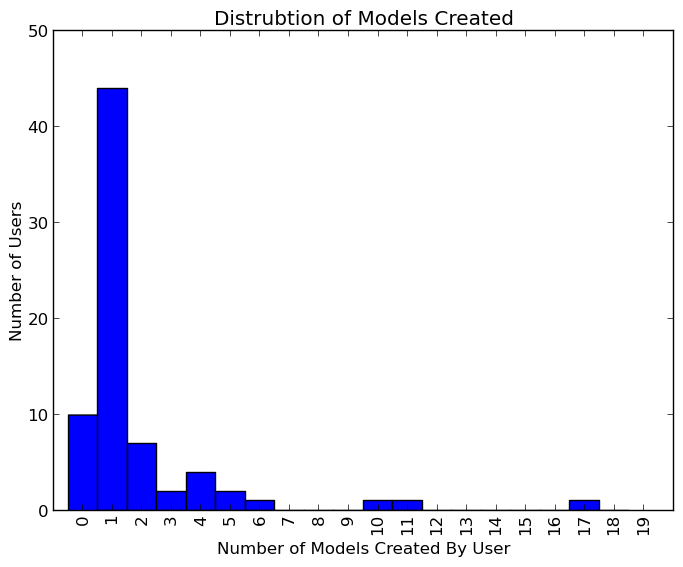
\includegraphics[width=0.8\textwidth]{model_hist}
	\caption{The distribution of models created on OASIS}
	\label{fig:model_hist}
\end{figure}


\begin{figure}[h]
	\centering
	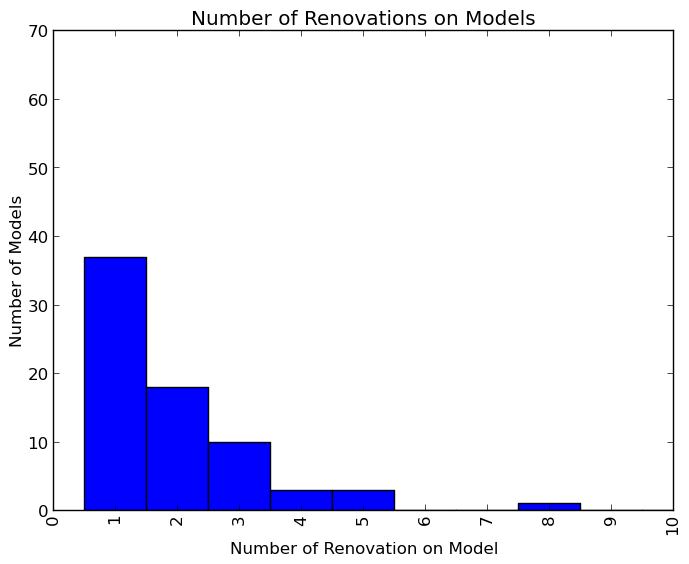
\includegraphics[width=0.8\textwidth]{renvo_hist}
	\caption{The distribution of renovations created on OASIS}
	\label{fig:renvo_hist}
\end{figure}

% \begin{figure}[h]
% 	\centering
% 	
\includegraphics[width=0.5\textwidth]{place_holder}
% 	\caption{Examples of some users created models on OASIS}
% 	\label{fig:examples}
% \end{figure}

\begin{figure}[h]
	\centering
	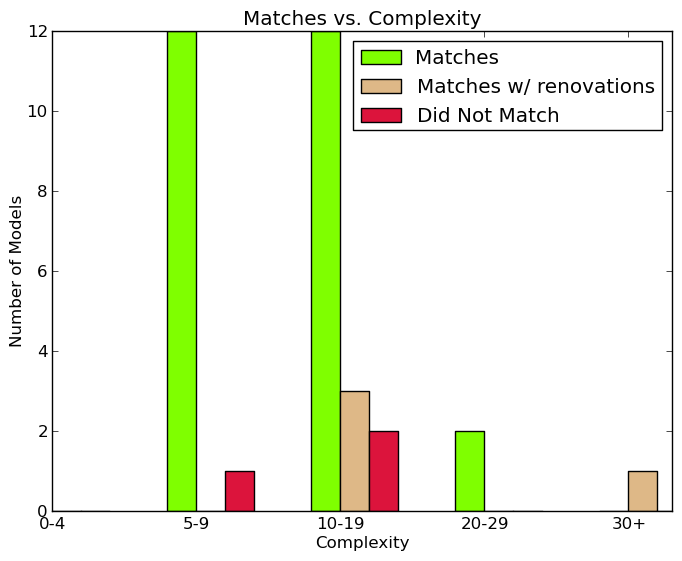
\includegraphics[width=0.8\textwidth]{matching_chart}
	\caption{Accuracy in relation to model complexity}
	\label{fig:matching_chart}
\end{figure}

After creating a 3D model participants can voluntarily provide feedback concerning the accuracy of our interpretation.
A participant can state if the  interpretation of their sketch initially matched their intention,  matched after performing adjustments, or did not a match at all.
I hypothesized that as models grew more complex the accuracy of our interpretation algorithm would decrease.
Figure-\ref{fig:matching_chart} illustrates model complexity in relation to matching user intentions.
For this investigation I define model complexity as the number of primitives used to create a sketch. This simple metric does not capture the shape complexity of a model.
Figure-\ref{fig:matching_chart} is interesting because models regardless of complexity seem to always match users initial intentions without requiring renovations.
Even models with 20 to 29 primitives seem to always match.
While the data suggest that our physical sketch interpretation algorithm is accurate, I believe that more feedback is required before any statistically significant conclusions can be drawn.
From our collected data is clear that participants do not answer this specific feedback question readily.
We believe users aren't consciously omitting this question because they are just excited to get into the daylight rendering phase.
In order to better gauge our accuracy, changes to the interface need to be made to persuade participants to answer this feedback question. \\




Aside from categorical quantitative feedback, we also ask participants to quantitatively describe their overall impressions of the system's effectiveness in the construction of 3D models from users' sketches; 
Table-\ref{fig:effective} displays results from this feedback questions.
Of the 16 participants that provided feedback on the effectiveness of the physical sketch interpretation algorithm, 14 stated that the system generally matched their intentions.
One participant stated that they only saw 2D versions of the interpretation.
I presume this could be caused from the user either not rotating their model or limited WebGL support on their web browser.
I do  not currently collect meta data on participants' web browsers or cursor movements, so currently there is no explanation for the problem encountered by this participant.
Two participants mentioned the lack of support for doors hindered the effectiveness of generating 3D models.
One participant linked us an image in their feedback, that displayed a rendering issue they had encountered.
The detail of some of the qualitative feedback provided from participants was higher than originally expected.
A take away from participants taking screen shots, hosting images online, and linking images of problem renderings to us is that OASIS should provide an easier means to associate feedback to models.

\begin{table}[h]
\centering
\begin{tabular}{|p{0.2\textwidth}|p{0.8\textwidth}|}
\hline
\rowcolor[HTML]{EFEFEF} 
\textbf{Username} & \textbf{Feedback} \\ \hline
qq & Can't make doors. Walls seem slanted in model visualization, which is probably intended. \\ \hline
Solyha & I still only see 2D \\ \hline
durkeejw & good, easy, fast \\ \hline
qjkxkcd & Model matched 2d representation from step 2. There was kind of a funky rendering issue (http://imgur.com/COBtYgv). (This was resolved when I remembered to add a final wall to close the room) + Also, when typing in this text box, using the arrow keys to navigate around text also pans the image around. \\ \hline
flowerJane & It was really fast and it rendered nicely \\ \hline
Jan Selz & Proportions of items and volume created seem to match the design intent. \\ \hline
mike smith & the program does a good job constructing the 3D model \\ \hline
ryasoa & It worked very well \\ \hline
damamani & Very good 3-D modeling but Step two needs some additional features to connect the walls properly. \\ \hline
principealberto & It is \\ \hline
tranthang & It well windows and furniture it is place windows fine \\ \hline
dcheung3 & Overall the 3D model does capture my sketch \\ \hline
alanlang & the 3D match my design \\ \hline
mindykay & This is really amazing! The 3D design is exactly what I was aiming for! \\ \hline
kyoko.usagi & I mean yes this kind of matches, but no doors is not in my intended design. That's why it failed. But the effectiveness is pretty spot on \\ \hline
galarodo & Accurate to the design.  Room was little bit wider (beds further apart) but requires to many edits to fix.  Deleting walls and redrawing them \\ \hline
\end{tabular}
\caption{Feedback to the question: Describe your overall impression of the system's effectiveness in constructing a 3D model from your design.}
\label{fig:effective}
\end{table}

Moreover, we asked users to describe cases where models were incorrectly interpreted by our physical sketch interpretation algorithm.
Table-\ref{fig:failure} present participant feedback about these failure cases.
Eight participants provided feedback on failure cases, however, some feedback provided is difficult to analyze.
Two  participants claim there were no issues in our interpretations of their sketches.
Particularly, three participants provided feedback making references to problems on specific models without images or model titles for us to associate the feedback with.
Only one participant provided a hyper-link to an image of a model they encountered problems with.
I suspect the other two participants believed OASIS kept track of which model users were viewing when providing feedback.
This particular feedback question is a general system wide question, so I did not anticipate that users would associate this question with the model currently being viewed by the participant.
Furthermore, another participant misinterpreted the question and stated that the lack of lofted beds in the system was a limitation to design.
Another participant was unhappy with design choices we made that deviate from standard modeling software conventions for viewing the 3D interpreted sketches. 
The main purpose of viewing the  3D interpretation of a sketch is to confirm that the interpretation matched users' intentions. As mentioned previously in section-\ref{3dviewer} future iterations of OASIS might do away with this viewer and incorporate it during user sketching.

Feedback on failure cases demonstrated the importance of linking feedback to models in the system rather then  simply describing those cases through just written feedback.
Descriptions of a failure cases without reference models proved to be ambiguous and unhelpful in  diagnosing users' issues.


\begin{table}[h]
\centering
\begin{tabular}{|p{0.2\textwidth}|p{0.8\textwidth}|}
\hline
\rowcolor[HTML]{EFEFEF} 
\textbf{Username} & \textbf{Feedback} \\ \hline
Solyha & There is no window on the west wall. The window in the center wall should not be the whole length of the wall only 0.75\% of the wall. \\ \hline
qjkxkcd & Part of the room is kind of an L-shape. When viewed from certain angles, it looks like one wall extends farther than it does in the 2d representation (http://imgur.com/qnGfydB). (Note: this was also fixed by completing the wall which was previously left open) + Also the window is only visible looking out from inside the room (the wall looks solid from the outside). +  And it might be by design, but the black circle base is only visible when looking at the model from above, not below. \\ \hline
mike smith & i did not find nothing wrong yet \\ \hline
damamani & The location of objects were placed accordingly to the sketch. \\ \hline
dcheung3 & one of the wall was not connecting \\ \hline
kyoko.usagi & No doors, like why no doors? \\ \hline
galarodo & No option to make a lofted bed that is the same height as the wardrobe! \\ \hline
raarming & the walls \\ \hline
\end{tabular}
\caption{Feedback to the question: Describe cases where the system incorrectly interpreted your design intentions.}
\label{fig:failure}
\end{table}



\section{Daylighting Analysis Feedback}


The final set of qualitative feedback I collect in our pilot user study, concerns participants' experience with daylighting in OASIS.
Specifically we ask participants if they understood the results of daylight simulations and to describe anything they found unclear or confusing about our visualizations.
Table-\ref{fig:understood} contains user feedback about participants' comprehension of simulation results.
Note that the feedback collected in Figure-\ref{fig:understood} is associated with a specific rendering.
I anticipated that users would understand some simulation results for a given rendering but not understand all simulation results. Accordingly, I made sure to associate this question with specific renderings for future analysis.
Surprisingly, participants' responses between renderings did not vary. 
Out of the 10 participants that provided feedback 9 claimed to understand simulation results.
One participant expected daylight from a north facing window at noon in the norther hemisphere;
This participant might not have known that there is no direct sunlight from northern-facing fenestrations in the northern hemisphere.
Users misconceptions about daylight are covered in a previous users study on the Virtual Heliodion.

\begin{table}[h]
\centering
\begin{tabular}{|p{0.2\textwidth}|p{0.8\textwidth}|}
\hline
\rowcolor[HTML]{EFEFEF} 
\textbf{Username} & \textbf{Feedback} \\ \hline
damamani & Simulation worked perfectly \\ \hline
alanlang & I understood the simulation \\ \hline
dcheung3 & Yes, I understand the results of the simulation. \\ \hline
h.tran1990 & Yes, this is very well thought out and it is a great program \\ \hline
flowerJane & I thought that maybe there would be light shining through since I set the time to  12 pm, but there was none \\ \hline
durkeejw & Yes, Straightforward \\ \hline
alanlang & i understood the simulation \\ \hline
dcheung3 & Yes, I understand the results of the simulation. From the data, it would seem that the rooms are over illuminated and this simulation clearly indicates as such. \\ \hline
ryasoa & I understood the results of the simulation. I think something that needs to be taken into consideration is the reflection of other buildings because while the simulation looks very nice + ( I prefer the dark at this time) my room is VERY bright at this time and I think it may be due to the surrounding building reflections \\ \hline
mindykay & Everything was perfect! As expected. The analysis part is really convenient as well! + I wish there was an ability to close the application to ensure my feedback was saved. I see it was saved because it says it at the bottom of the screen, but it be nice to have an exit button to close the window and ensure that all feedback was marked down. \\ \hline
\end{tabular}
\caption{Feedback to the question: Did you understand the results of the simulation? Describe anything confusing or unclear.}
\label{fig:understood}
\end{table}

Lastly we asked participants if the system allowed them to test daylighting performance and if they understood over and under illumination visualizations. Figure-\ref{fig:effective} shows that of the 10 participants that provided feedback, seven participants provided positive statements. In general, participants understood over and under illumination and claimed that OASIS was useful for daylighting performance and analysis. Interestingly, our most experienced user claimed that OASIS was not effective for daylighting analysis.The user stated that they did not understand what under and over illumination thresholds were relative to. OASIS does not currently support adjusting thresholds for under and over illumination. Adjusting these thresholds for common activities, such as office work, are left as future implementation.In the course of this pilot user study, the feedback from our participant with over 10 years work experience in architecture was constructive. Similarly, the feedback from the non-experts is invaluable in regards to future user interface decisions.

\begin{table}[h]
\centering
\begin{tabular}{|p{0.2\textwidth}|p{0.8\textwidth}|}
\hline
\rowcolor[HTML]{EFEFEF} 
\textbf{Username} & \textbf{Response} \\ \hline
rolyha@verizon.net & yes \\ \hline
Solyha & No- it's very dark for 1 pm \\ \hline
durkeejw & No. What light levels are considered ``over'' or ``under''? \\ \hline
Jan Selz & I can see a small amount of illumination in the corner.  It does make sense for only having a North facing window. \\ \hline
mike smith & the program works as i expected \\ \hline
ryasoa & Yes, understood both \\ \hline
tranthang & Yes, it is great simulations and a great experience \\ \hline
dcheung3 & Yes, the system allowed me to create and test daylighting performance. Yes i have a better understanding the area of over illumination and under illumination. \\ \hline
mindykay & Yes, this application definitely shows how my space would be illuminated \\ \hline
alanlang & the simulation was clear. \\ \hline
\end{tabular}
\caption{Feedback to the question: Did the system allow you to create and test daylighting performance? Do you understand the areas of over illumination and under illumination?}
\label{fig:effective}
\end{table}


































    \chapter{Conclusion and Future Works} \label{sec:results}

\section{Conclusion}
We performed a pilot user study to determine if OASIS was accessible, easy-to-use, and a step in the right direction as an early design tool for daylighting.
Firstly, feedback from the study, which spanned only 2 weeks, demonstrates OASIS was accessible to a board range of users outside of the tradition pool of architecture students used in previous user studies\cite{}.
Similarly, there was no feedback concerning problems with accessing our online sketching interface.
Secondly, user feedback from our pilot user study showed that OASIS was both easy-to-use and fun.
However, it is also important to note that our pool of participants consist mostly of non-experts. 
Whether our sketching interface was easy to use for experts remains unknown.
Lastly, most feedback collected from participants concerning the effectiveness of OASIS for daylighting analysis was positive -- with over 90\% of participants stating that OASIS was effective and clear.
Conversely, one participant with 10+ years job experience in architecture stated that OASIS was not useful for daylight analysis.
This participant, however, was not clear as to why OASIS was not effective for daylighting analysis.
Before any conclusion can be drawn, I believe we need to collect more feedback from experts and advertise our online tool towards users with architectural experience.
In brief my contributions include the creation of a novel architectural sketching interface for simulations that is both accessible and easy-to-use for non-experts to perform qualitative daylighting analysis.
In addition I conducted an online pilot user study and analyzed the results from that study.
Moreover, I created an online framework for the physical sketch interpretation algorithm and daylight rendering engine used in the Virtual Helidon.

\section{Future Work}

\subsection{Improved Evaluations of OASIS}
My pilot user study was meant to be a short study to test key features of OASIS and understand problems users would encounter when using OASIS.
Future user studies aimed at evaluating future iterations of OASIS in more detail can learn from mistakes made in this pilot user study.
Firstly, the amount of users who registered and did not create a single model on OASIS is high.
Despite lack of data on the retention rate of similar user studies, there are a few strategies that can be used to increase the number of users on OASIS.
Goal driven user feedback may increase users interest in creating models on OASIS, sharing those models, and providing insightful feedback. 
Disguising user studies as goal driven games has had successes in the crowd sourcing line drawings in previous research\cite{}.
Having users use OASIS to fix a problem caused by daylighting, such glare in an office, with a scoring mechanism might incentive users to use OASIS as experts would. 
Coupled with sharing features, that let users share 3D models or their scores would help OASIS self advertise itself to other users.
Additional, making registration easier or even optional, for the first model, could increase user retention.
Similarly, in our pilot study we encountered problems user made assumptions about feedback and models being viewed.
Adding in a share feature, such as an automatically generated link that displays a model, would make sharing problem models much easier in feedback responses.
Lastly, there was problem with users omitting feedback that could potentially communicate something to researchers.
Making some feedback questions non-optional or inbreeding the feedback into the interface would make user intentions clearer.

\subsection{Improvements To The Online Sketching Interface}
Despite my original hypothesis not being met, the pilot user study did provide us feedback about what usability features to prioritize for future work.
Firstly, the most requested feature in our sketching interface was support for doors.
As mentioned previously, the physical sketch interpretation algorithm can interpret multi-room sketches.
However, the lack of doors on the sketching interface communicated that we do not support multi-rooms sketches to many of our users.
Additionally, the study revealed that room designs were greatly limited by the small number of furniture items in the system.
While, OASIS is not meant to be a fully features daylighting analysis software, providing user a wider variety of furniture items would aide in the design of spaces other than bedrooms.
Another common concern was scale, users wanted either control of scale in their sketches or more explicit communication of scale in our sketching interface.
Giving users control of scale and providing an overlay of grid-lines on the sketching interface might better communicate scale of architectural spaces better than the currently indirect sense of scale through statically sized furniture items.

Unrelated to results from our user study, OASIS is an online sketching interface for simulations. As of right now, the only true sketching features we support are straight walls. 
Future work can be done to make our interface a full support sketching environment.
Users in this sketching environment can draw not only straight walls, but also curved walls of any shape, in addition to sketching in windows and furniture items, similar to LightSketch\cite{}.
Such a system would require some form of sketch recognition and a vocabulary or training sketches for common furniture items.
Advantage so such a system would be one step closer to emulating how architects currently plan daylighting in the early design phase through rough pencil and paper sketches.

\subsection{Improvements To Daylighting Visualizations}
OASIS incorporates the daylight rendering engine from the Virtual Heliodon.
The daylight rendering engine uses a GPU ray tracing framework, known as NVidia Optix\cite{}, to perform photon mapping at interactive rates.
In the pipeline of the daylight rendering engine standard daylighting metrics such as the daylight factor, daylighting glare probability, and luminous flux per unit area, can be calculated and visualized in various ways.
Future work can focus on creating informative daylight visualizations optimized for our online viewer.\\




    %%%%%%%%%%%%%%%%%%%%%%%%%%%%%%%%%%%%%%%%%%%%%%%%%%%%%%%%%%%%%%%%%%%
%                                                                 %
%                           BIBLIOGRAPHY                          %
%                                                                 %
%%%%%%%%%%%%%%%%%%%%%%%%%%%%%%%%%%%%%%%%%%%%%%%%%%%%%%%%%%%%%%%%%%%

\newpage

\renewcommand\bibname{REFERENCES}

\begin{singlespace}
    \addcontentsline{toc}{chapter}{REFERENCES}
    % \bibliographystyle{IEEEtranSN_custom}
    \bibliographystyle{IEEEtran_custom}
    \bibliography{references}{}
\end{singlespace}



    \newpage
    %%%%%%%%%%%%%%%%%%%%%%%%%%%%%%%%%%%%%%%%%%%%%%%%%%%%%%%%%%%%%%%%%%%
%                                                                 %
%                            APPENDICES                           %
%                                                                 %
%%%%%%%%%%%%%%%%%%%%%%%%%%%%%%%%%%%%%%%%%%%%%%%%%%%%%%%%%%%%%%%%%%%

\appendix    % This command is used only once!

% \addcontentsline{toc}{chapter}{APPENDIX}             %toc entry  or:
% \addtocontents{toc}{\parindent0pt\vskip12pt APPENDIX} %toc entry, no page #

% \setcounter{table}{0}
% \renewcommand{\thetable}{A\arabic{table}}

% \setcounter{figure}{0}
% \renewcommand{\thefigure}{A\arabic{figure}}

\chapter{APPENDIX} \label{sec:appendix}

\section{User-Specific Questions}

\begin{enumerate}  
\item Are you affiliated with Rensselaer Polytechnic Institute? 
\item How are you affiliated with Rensselaer Polytechnic Institute?
\item Years of formal education in Architecture?
\item Years of formal education in Visual Arts?
\item Years of job experience in architecture? (including internships) 
\item Years of job experience in Visual Arts? (including internships)
\item Have you used any of the following modeling software?
\begin{enumerate}  
  \item SketchUp
  \item AutoCAD
  \item Rhino
  \item Maya
  \item 3DS Max
  \item Cinema 4D
  \item Blender
  \item Revit
  \item Other
\end{enumerate}
\item Years of experience with modeling software?
\item Other relevant education / experience?
\item Are you colorblind?
\item Is it okay if we follow up with additional questions about specific models you created in our system?
  \begin{enumerate}
    \item If so, please enter your email address
  \end{enumerate}

\item What did you find fun or interesting in this sketching environment?
\item What additional features should be added to system to allow greater flexibility in design?
\item Describe some designs that you were not able to create due  to system limitations?
\item Was there anything you did not like about working in this sketching environment?
\item Where there any UI elements that were hard to use or confusing at first?

\item Describe your overall impression of the software for determining the interior vs exterior space in your designs?
\item For the cases when the system’s interpretation of the interior/exterior of your design was incorrect where was the system wrong? 
\item Did the system allow you to create and test daylighting performance with respect to over or under illumination?

\end{enumerate}

\section{Model-Specific Questions}

\begin{enumerate}
\item What category does this model fall into?
\begin{enumerate}
  \item Dorm
  \item Bedroom
  \item Living room 
  \item Apartment / House
  \item Classroom
  \item Office
  \item Lobby
  \item Other
\end{enumerate}
% If it is an rpi dorm 
\item What dorm is this a model of? (Optional)
\begin{enumerate}
\item BARH (Burdett Avenue Residence Hall)
\item Barton Hall
\item Beman Lane Undergraduate RAHP Apartments
\item Blitman Residence Commons
\item Bray Hall
\item Bryckwyck Floor Plans
\item Cary Hall
\item Colonie Apartments
\item Commons
\item Crockett Hall
\item Davison Hall
\item E-Complex
\item Hall Hall
\item Nason Hall
\item North Hall
\item Nugent Hall
\item Quadrangle (The Quad)
\item Sharp Hall
\item Single RAHP
\item Stacwyck Apartments
\item Warren Hall
\item Other
\end{enumerate}
\item What floor number? (Optional)
\item What room number? (Optional)
\item When was the last time you visited this space? (Optional)
\begin{enumerate}
\item Less than a week ago
\item Less than a month ago
\item Less then a year ago
\item Less than 4 years ago
\item More than 4 years ago
\end{enumerate}
\item How often did you visit this space?
\begin{enumerate}
\item Once
\item Occasionally
\item Multiple times a week
\end{enumerate}
\item How confident are you in modeling this space? (scale of 1 to 5)

\end{enumerate}


\section{Renovation-Specific Questions}
\begin{enumerate}
\item Does the 3D generated model match your intentions?
\begin{enumerate}
\item Matched my intentions exactly ( no revision required )
\item Did not match my intentions initially ( revisions were required )
\item Failed to match my intentions ( even after revision )
\end{enumerate}
\end{enumerate}

\section{Render-Specific Questions}
\begin{enumerate}
\item Did you understand the results of the simulation, was there anything confusing or unclear?
\end{enumerate}


\end{document}
